\chapter{Search I: Limits per mass category}
\vspace*{\fill}\newpage
\section{Limits per mass category}
\label{app:search1}
The asymptotic limits obtained with 2.6 $\textrm{fb}^{-1}$ of 13 TeV CMS data per mass and purity category.
\begin{figure}[h!]
\centering
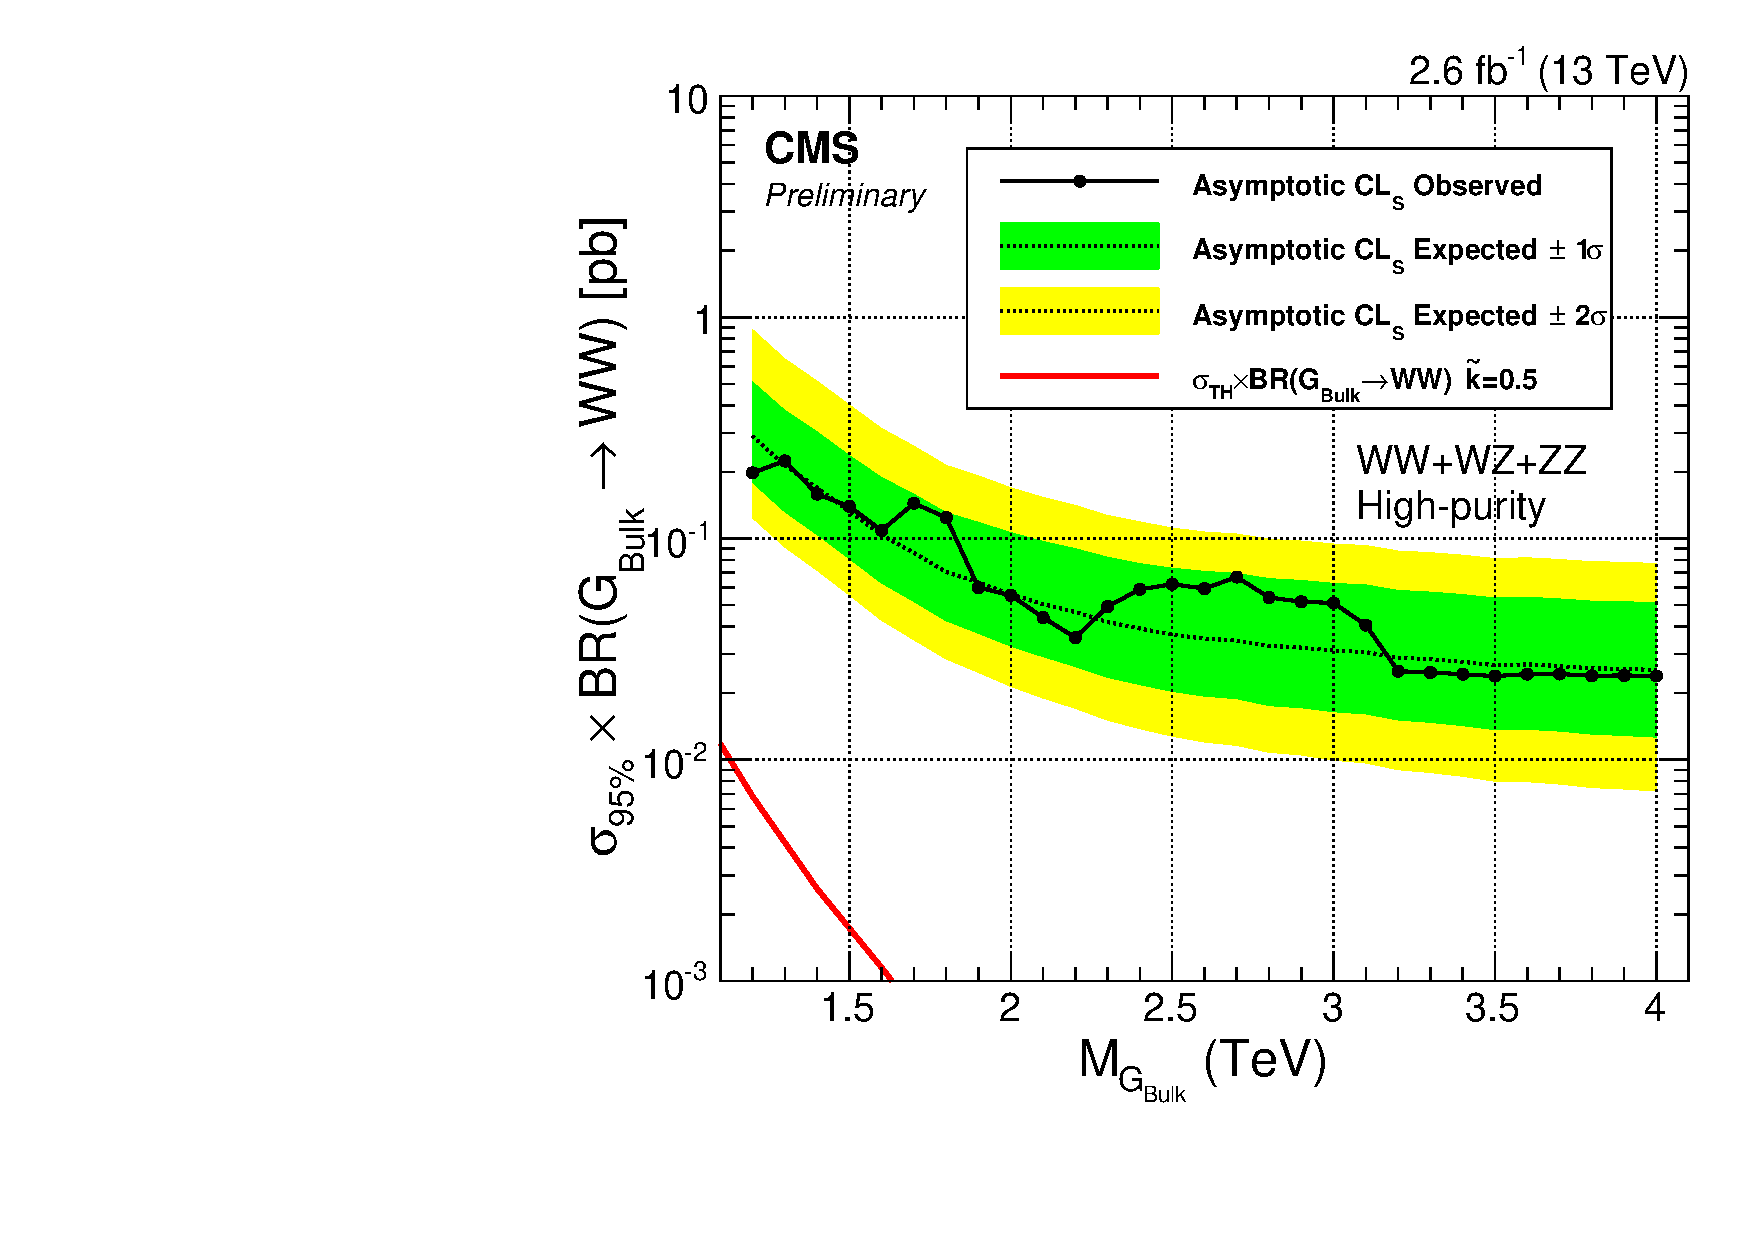
\includegraphics[width=0.327\textwidth]{figures/analysis/search1/AN-15-211/limits/brazilianFlag_BulkWW_VVHP_new_combined_purity_13TeV_wPDF.pdf}
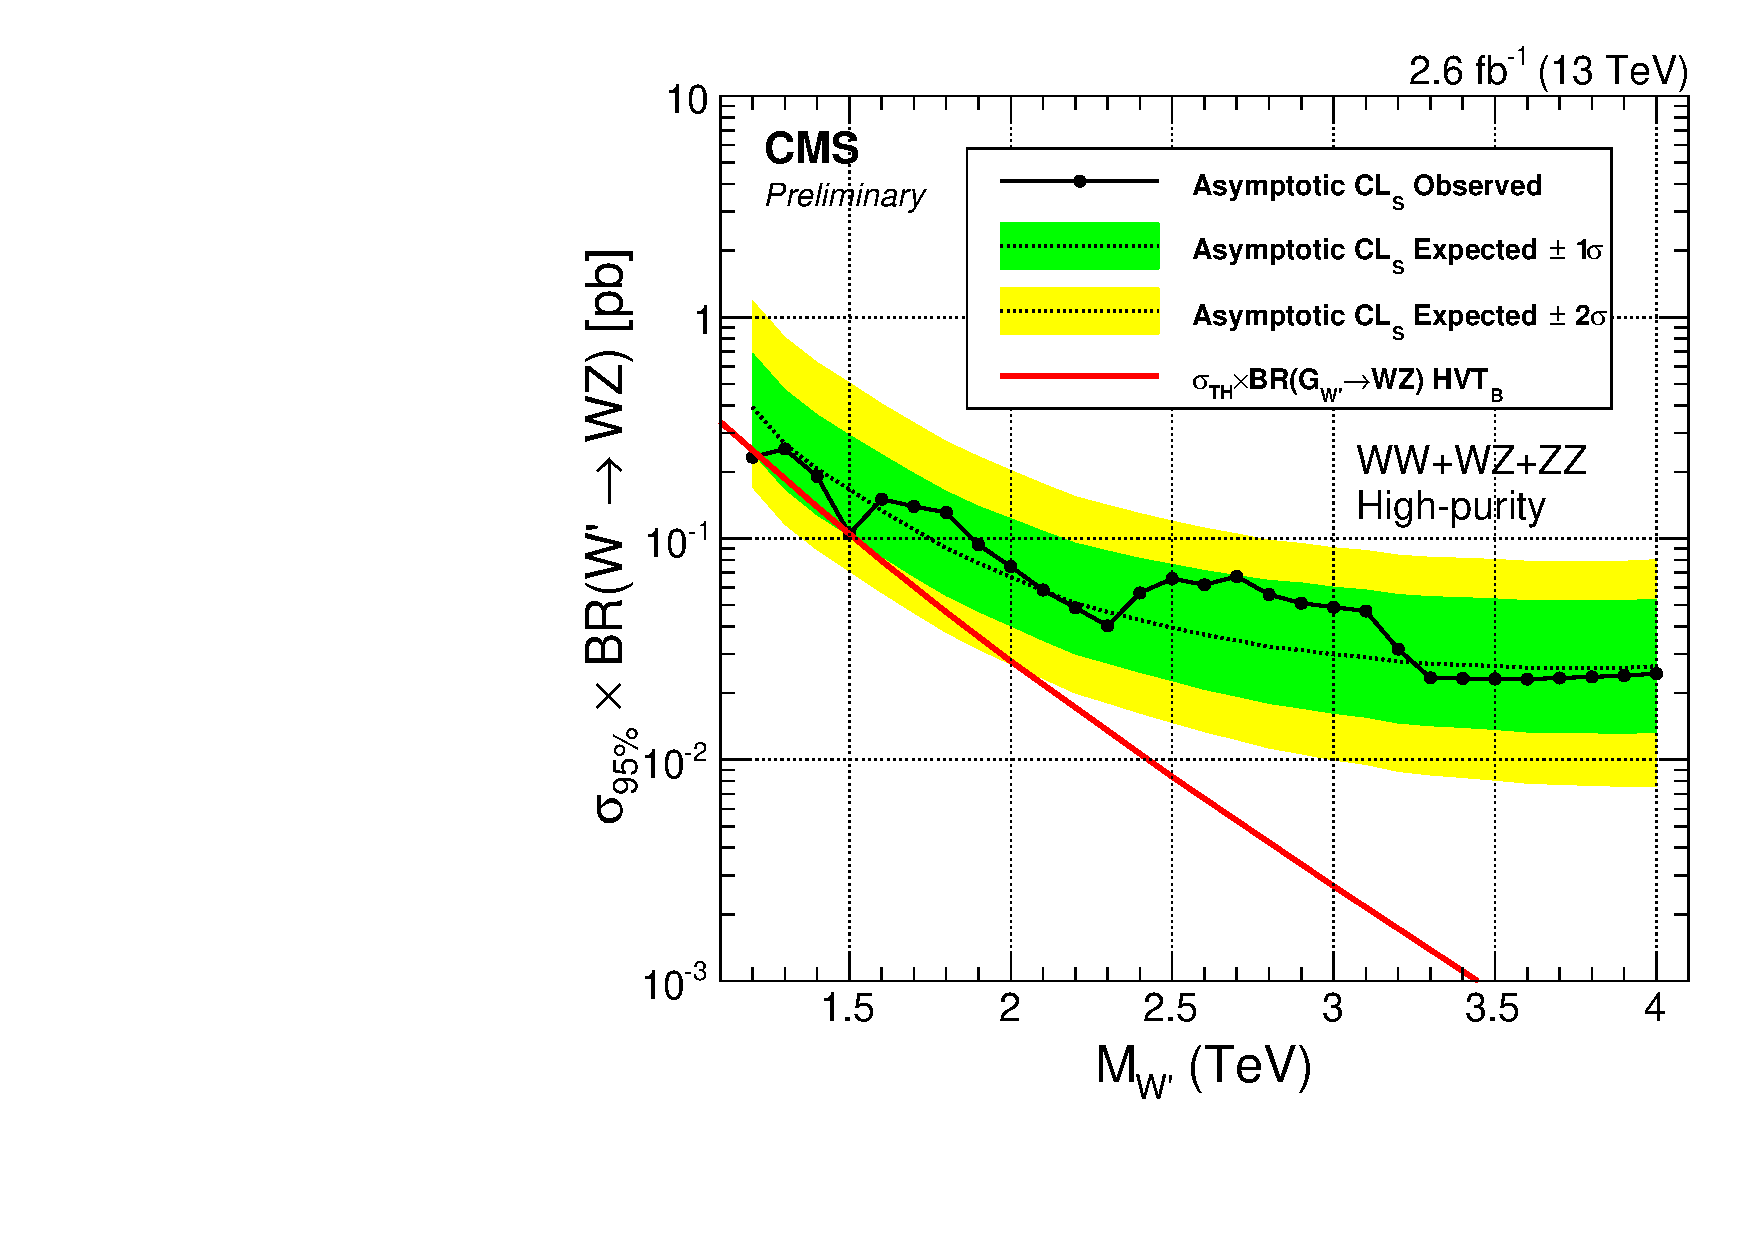
\includegraphics[width=0.327\textwidth]{figures/analysis/search1/AN-15-211/limits/brazilianFlag_WZ_VVHP_new_combined_purity_13TeV_wPDF.pdf}
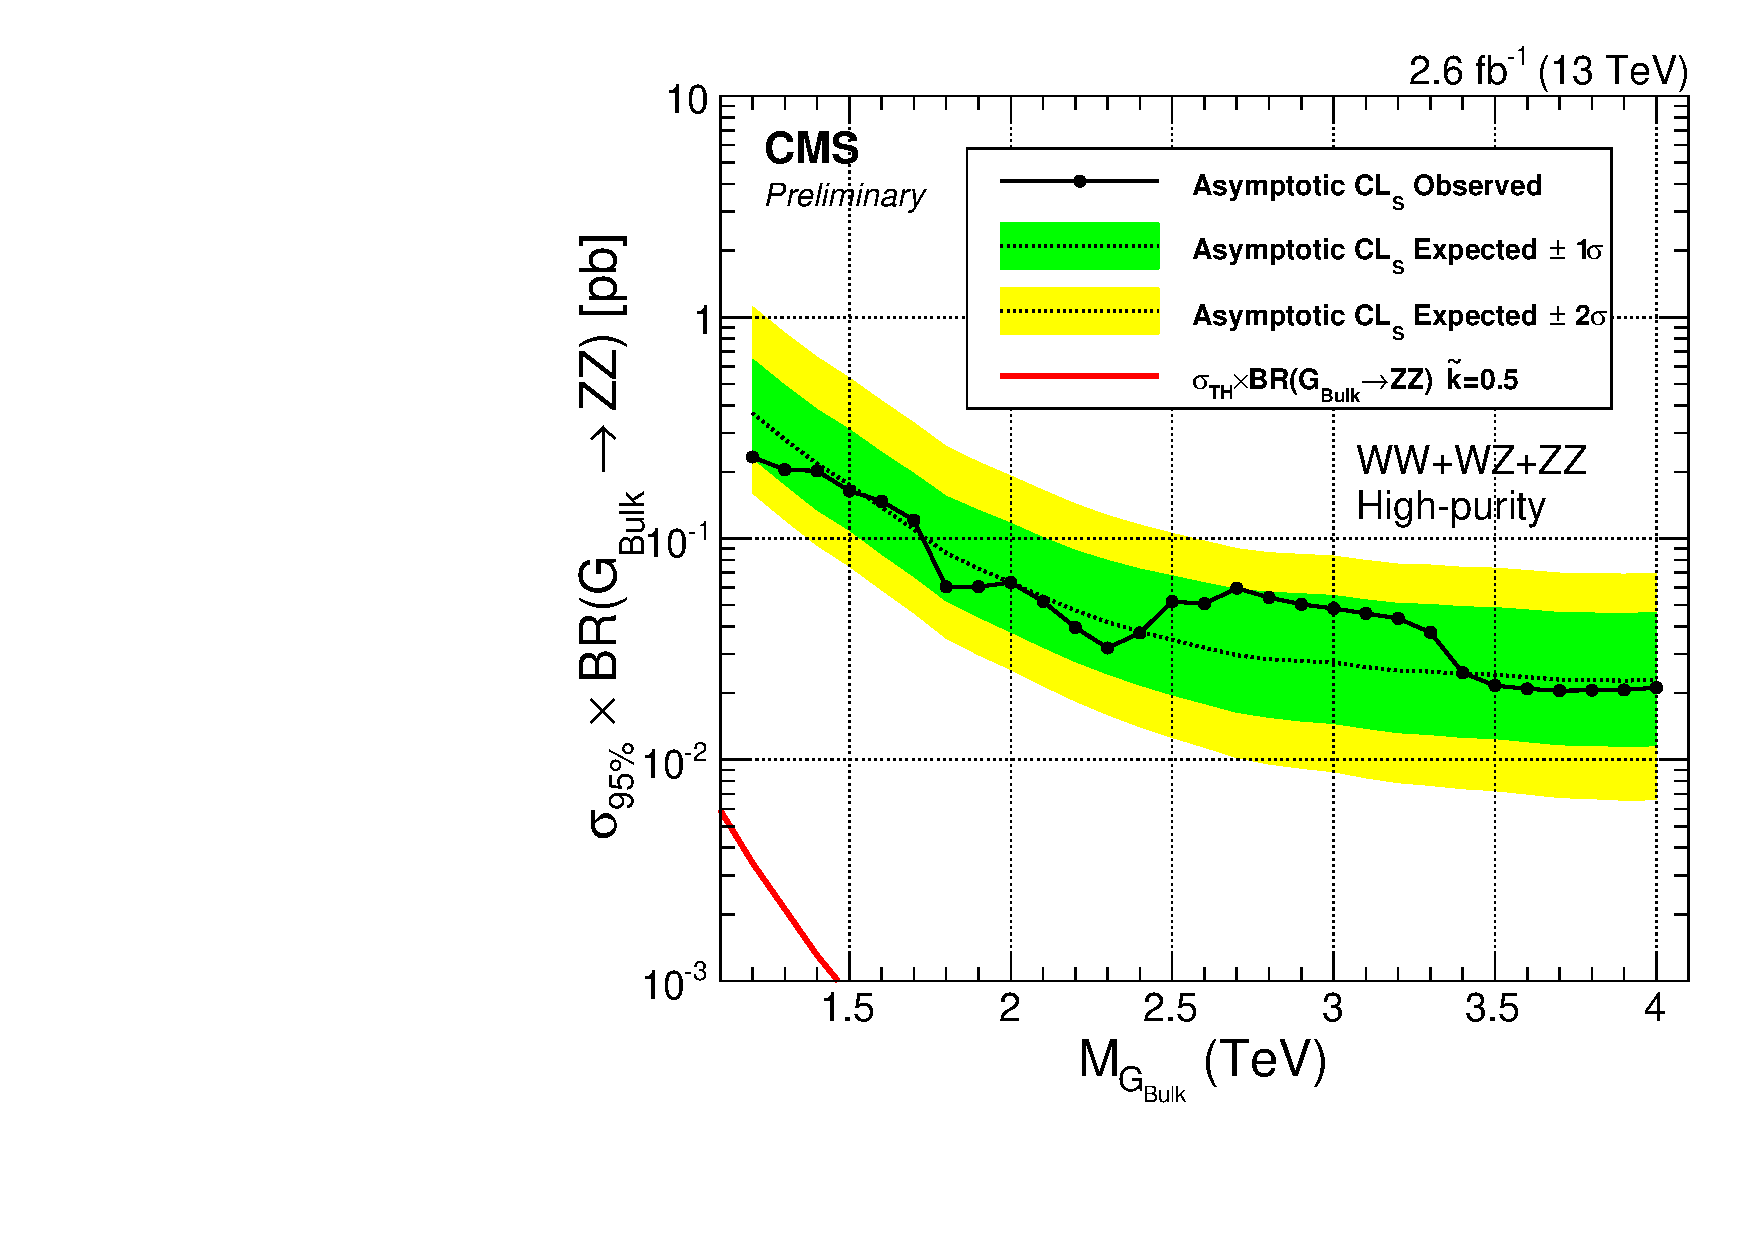
\includegraphics[width=0.327\textwidth]{figures/analysis/search1/AN-15-211/limits/brazilianFlag_BulkZZ_VVHP_new_combined_purity_13TeV_wPDF.pdf}\\
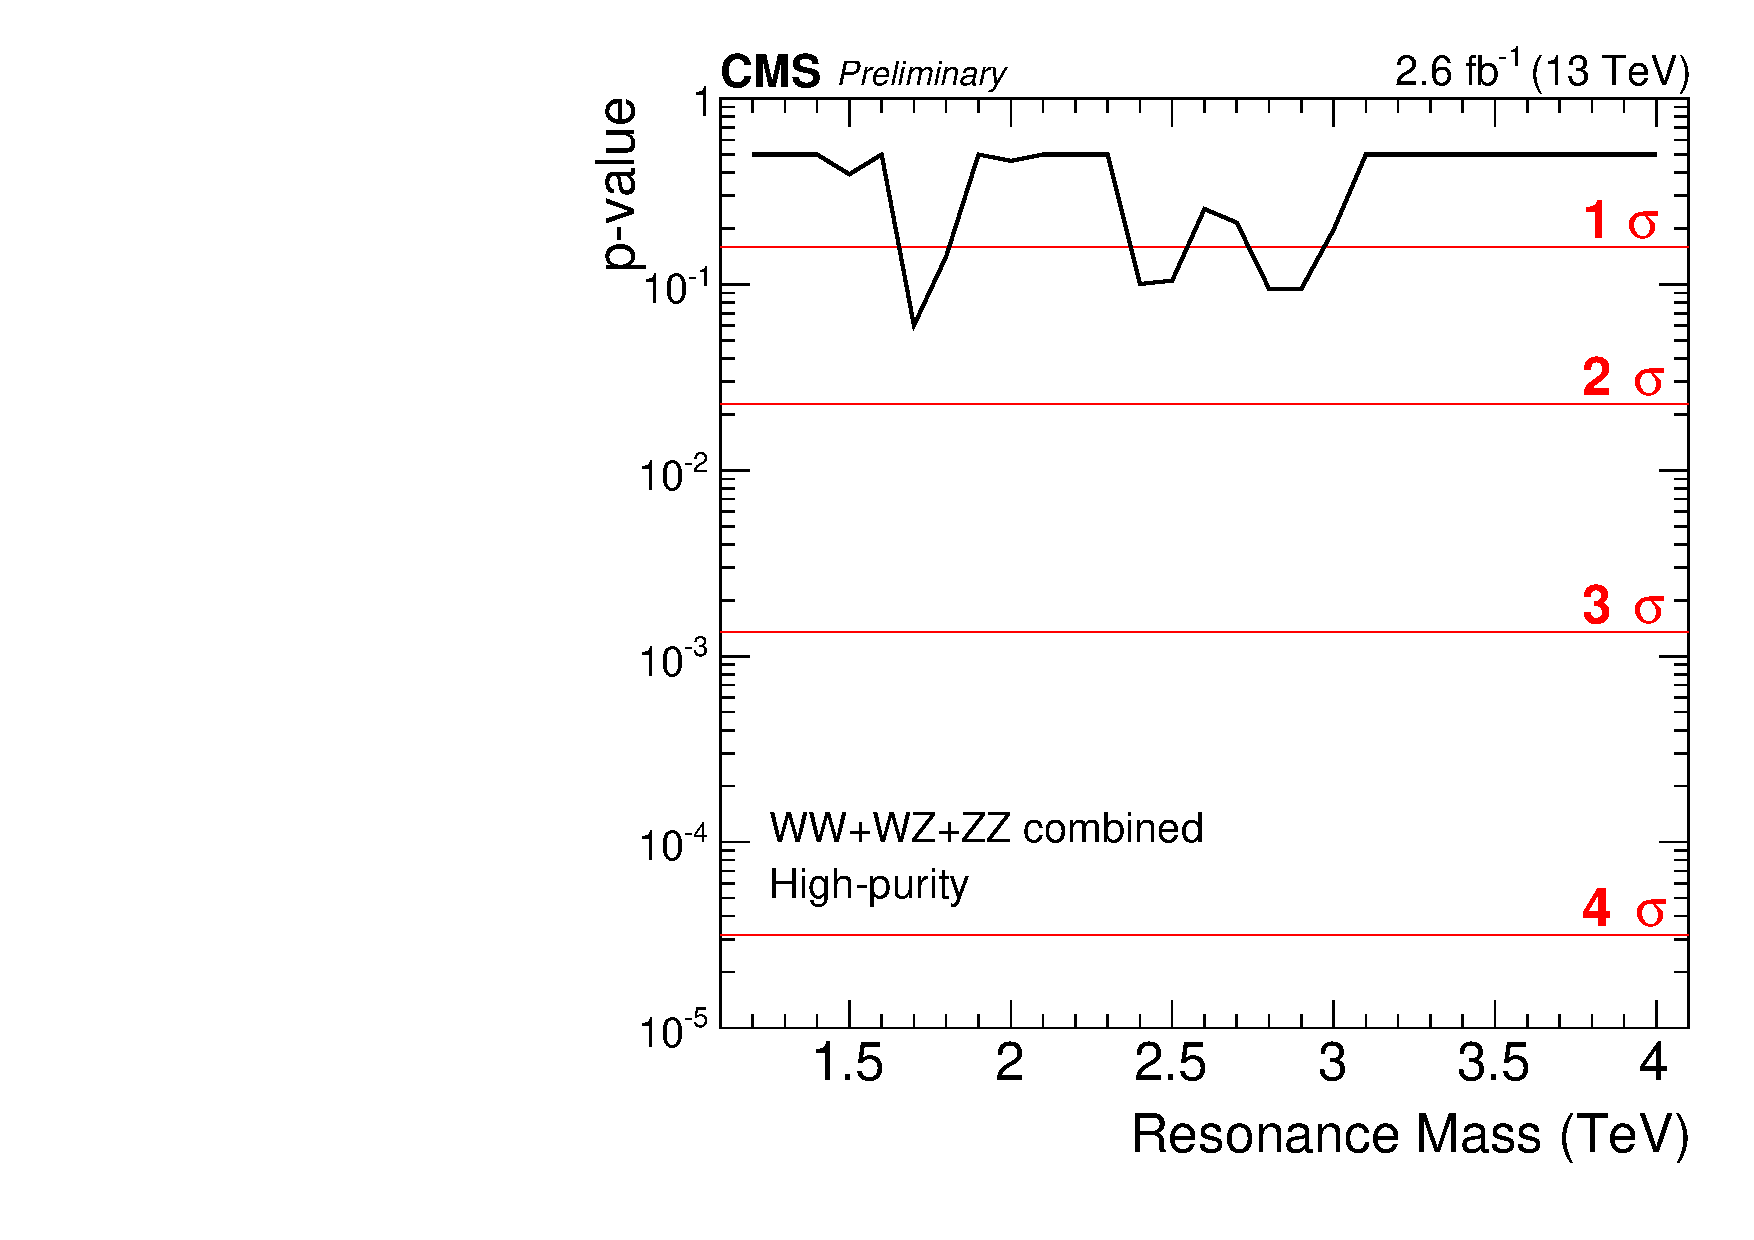
\includegraphics[width=0.327\textwidth]{figures/analysis/search1/AN-15-211/pvalues/pvalue_BulkWWinVVnew_high_purity.pdf}
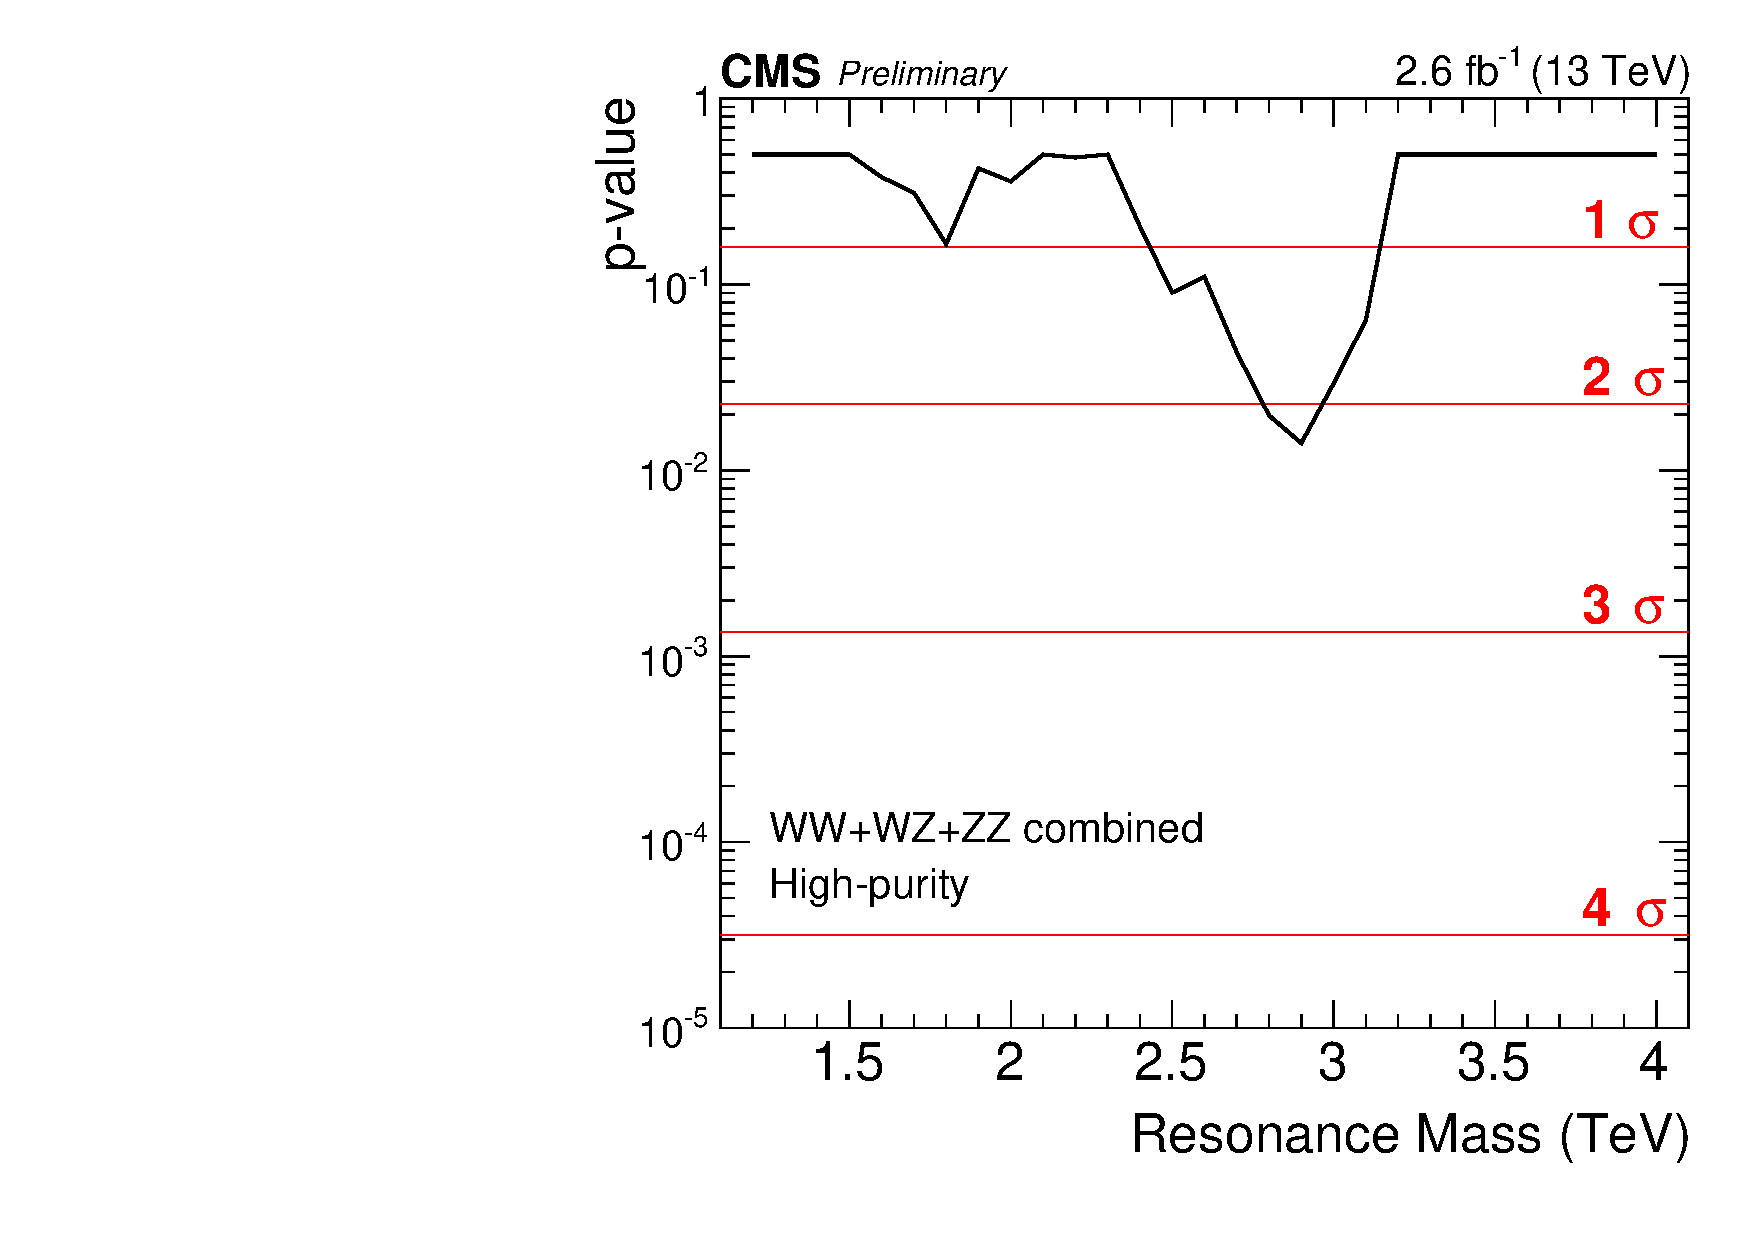
\includegraphics[width=0.327\textwidth]{figures/analysis/search1/AN-15-211/pvalues/pvalue_WZinVVnew_high_purity.pdf}
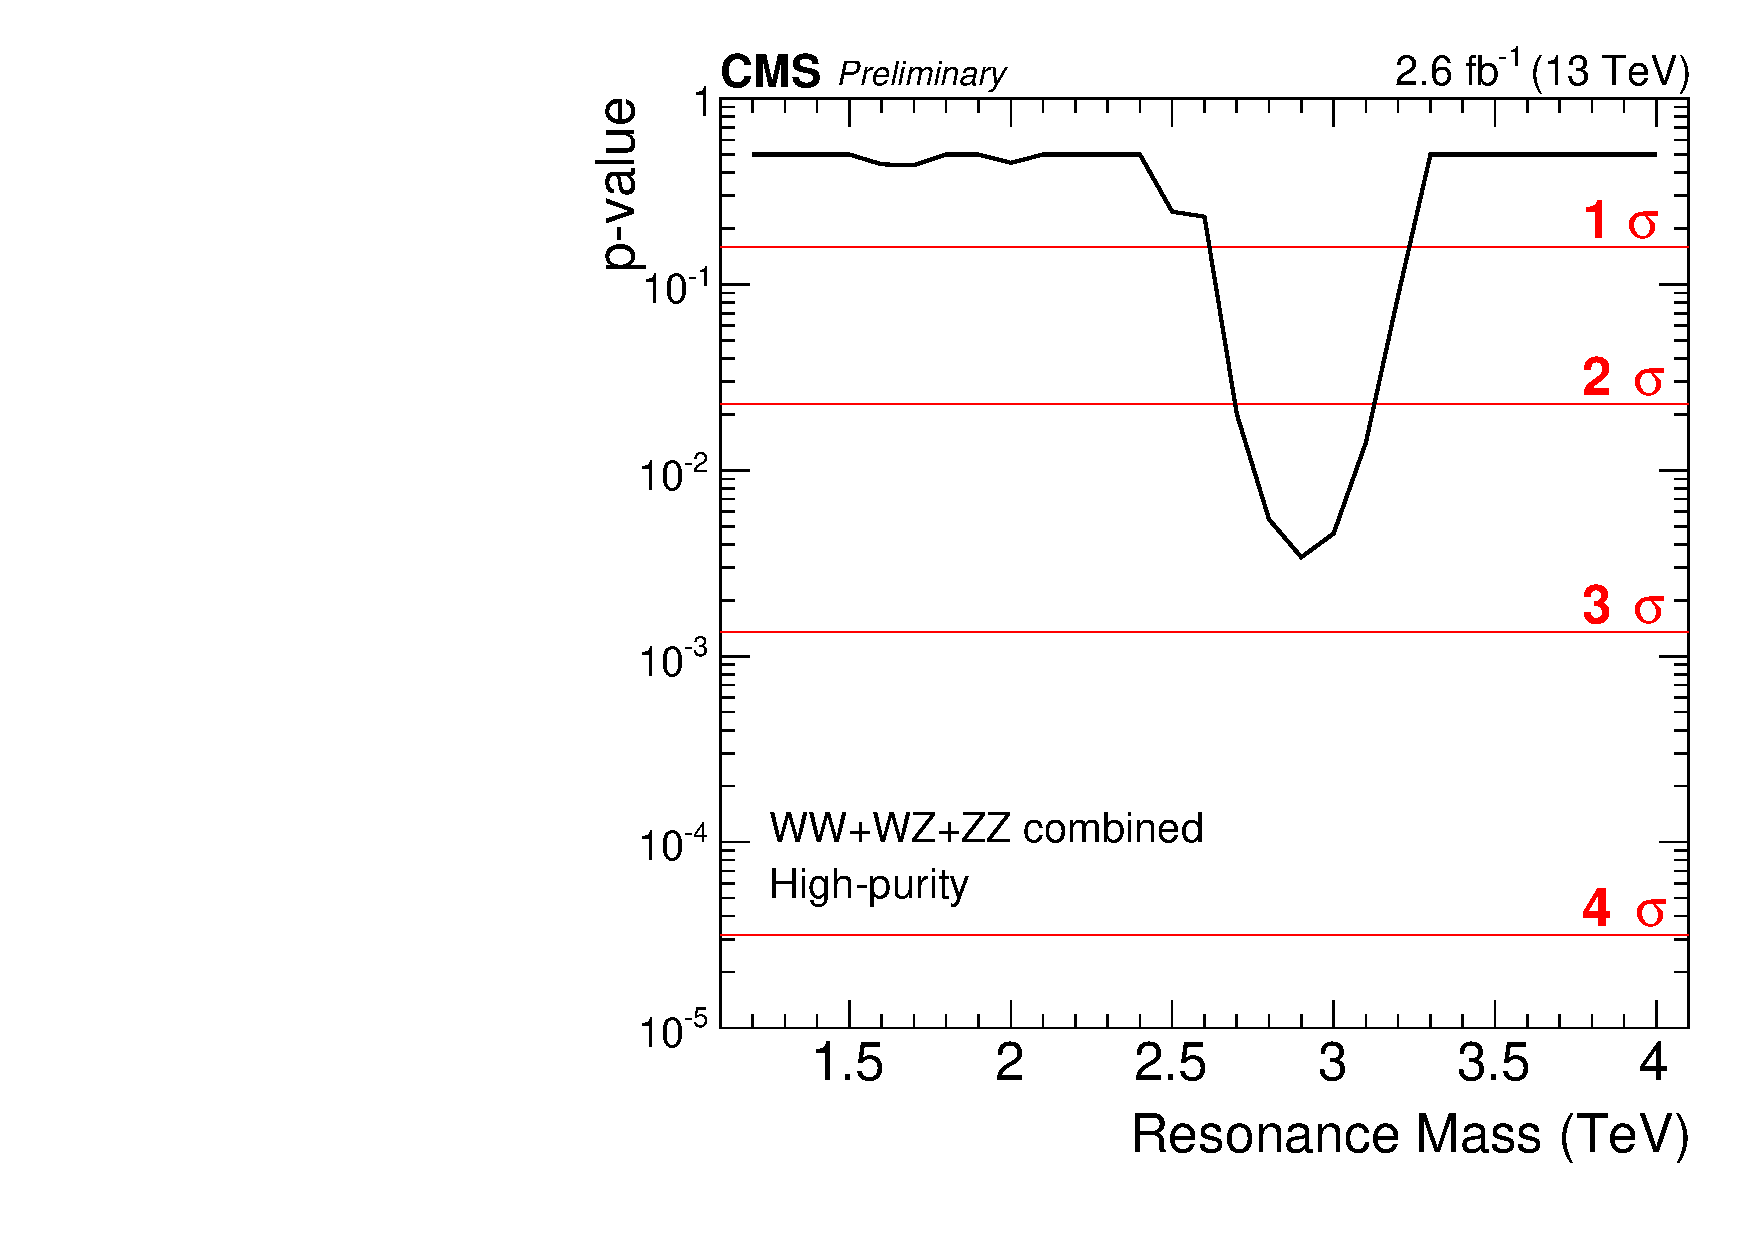
\includegraphics[width=0.327\textwidth]{figures/analysis/search1/AN-15-211/pvalues/pvalue_BulkZZinVVnew_high_purity.pdf}
\caption{Expected and observed limits at 95\% CL and corresponding p-values obtained in the high purity category using 2.6 $\textrm{fb}^{-1}$ of CMS data. Here for a Bulk $G\rightarrow WW$ (left), $W'\rightarrow WZ$ (middle) and $G\rightarrow ZZ$ (right) signal.}
\label{fig:app:Limits_HP}
\end{figure}
\begin{figure}[h!]
\centering
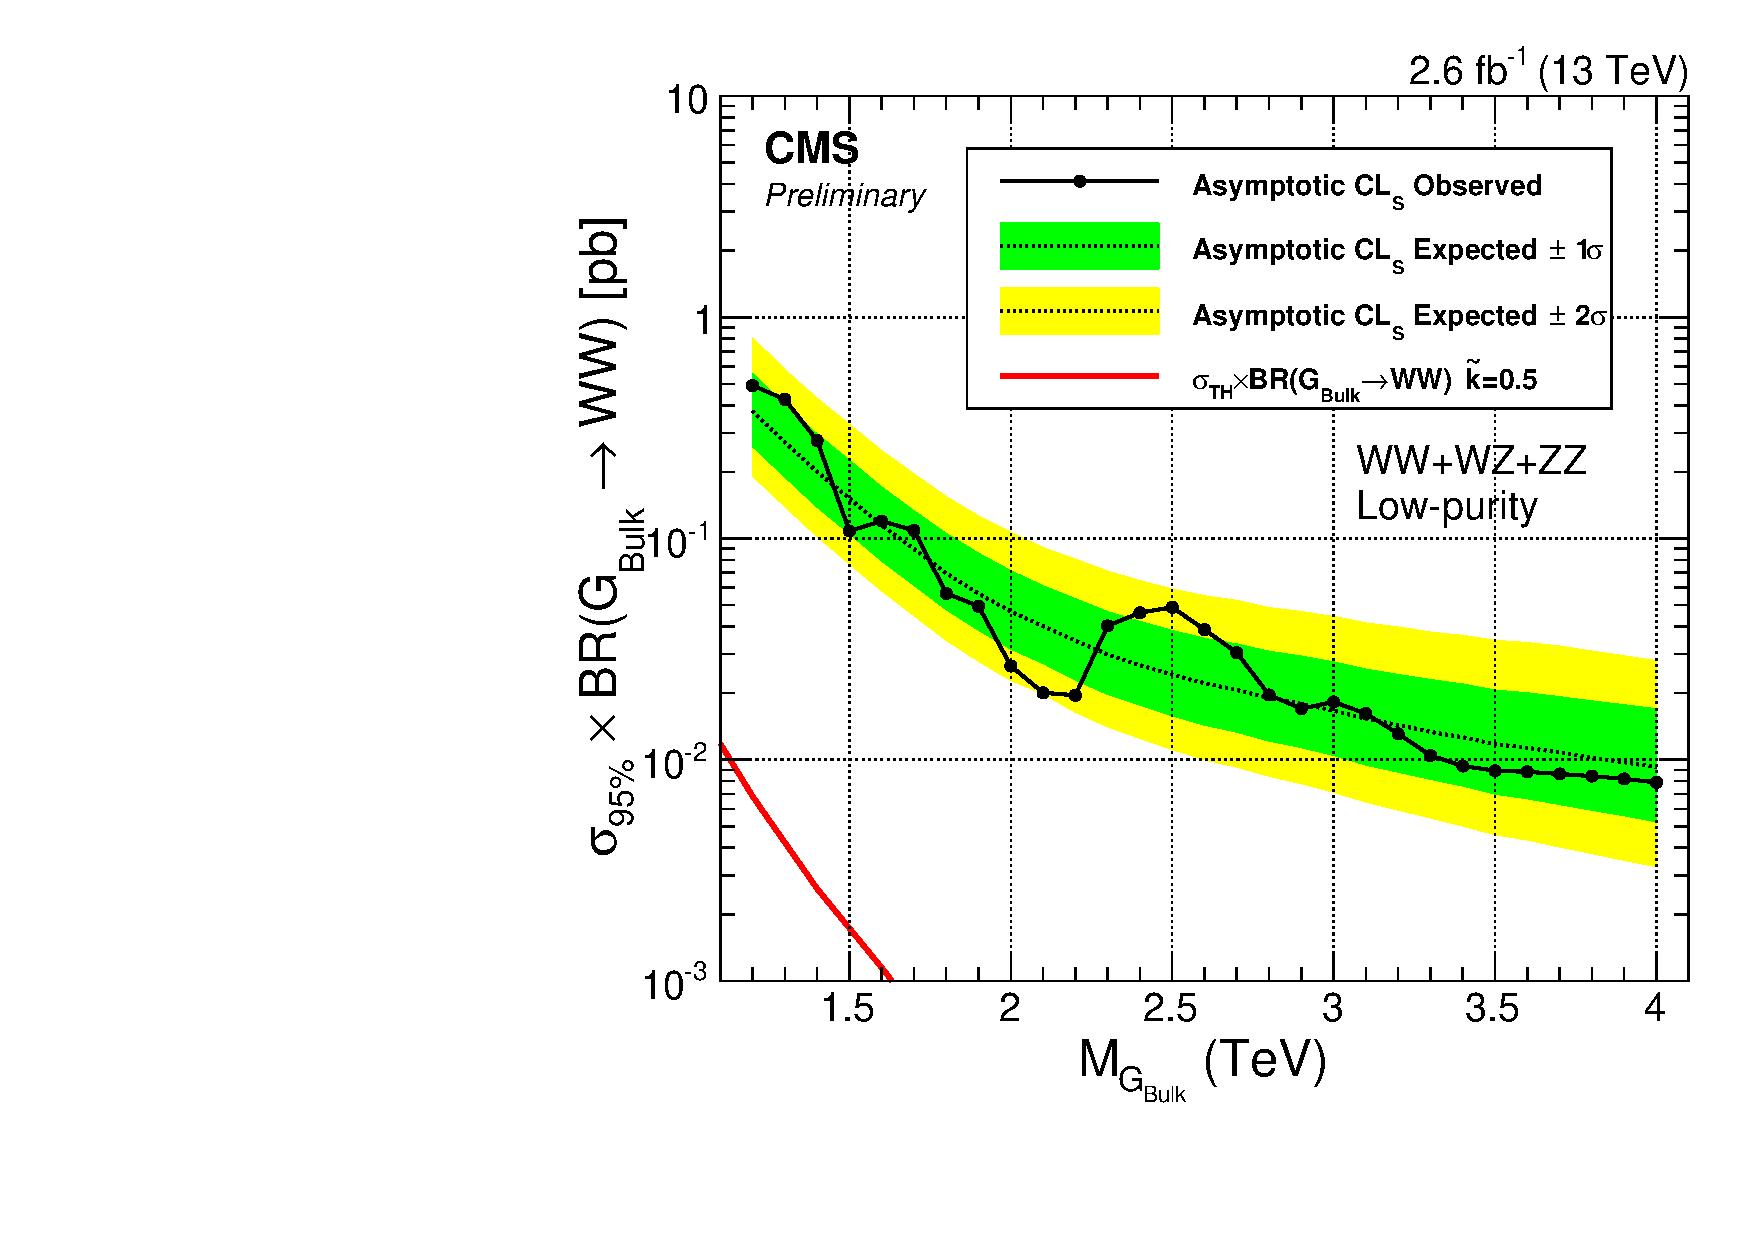
\includegraphics[width=0.327\textwidth]{figures/analysis/search1/AN-15-211/limits/brazilianFlag_BulkWW_VVLP_new_combined_purity_13TeV_wPDF.pdf}
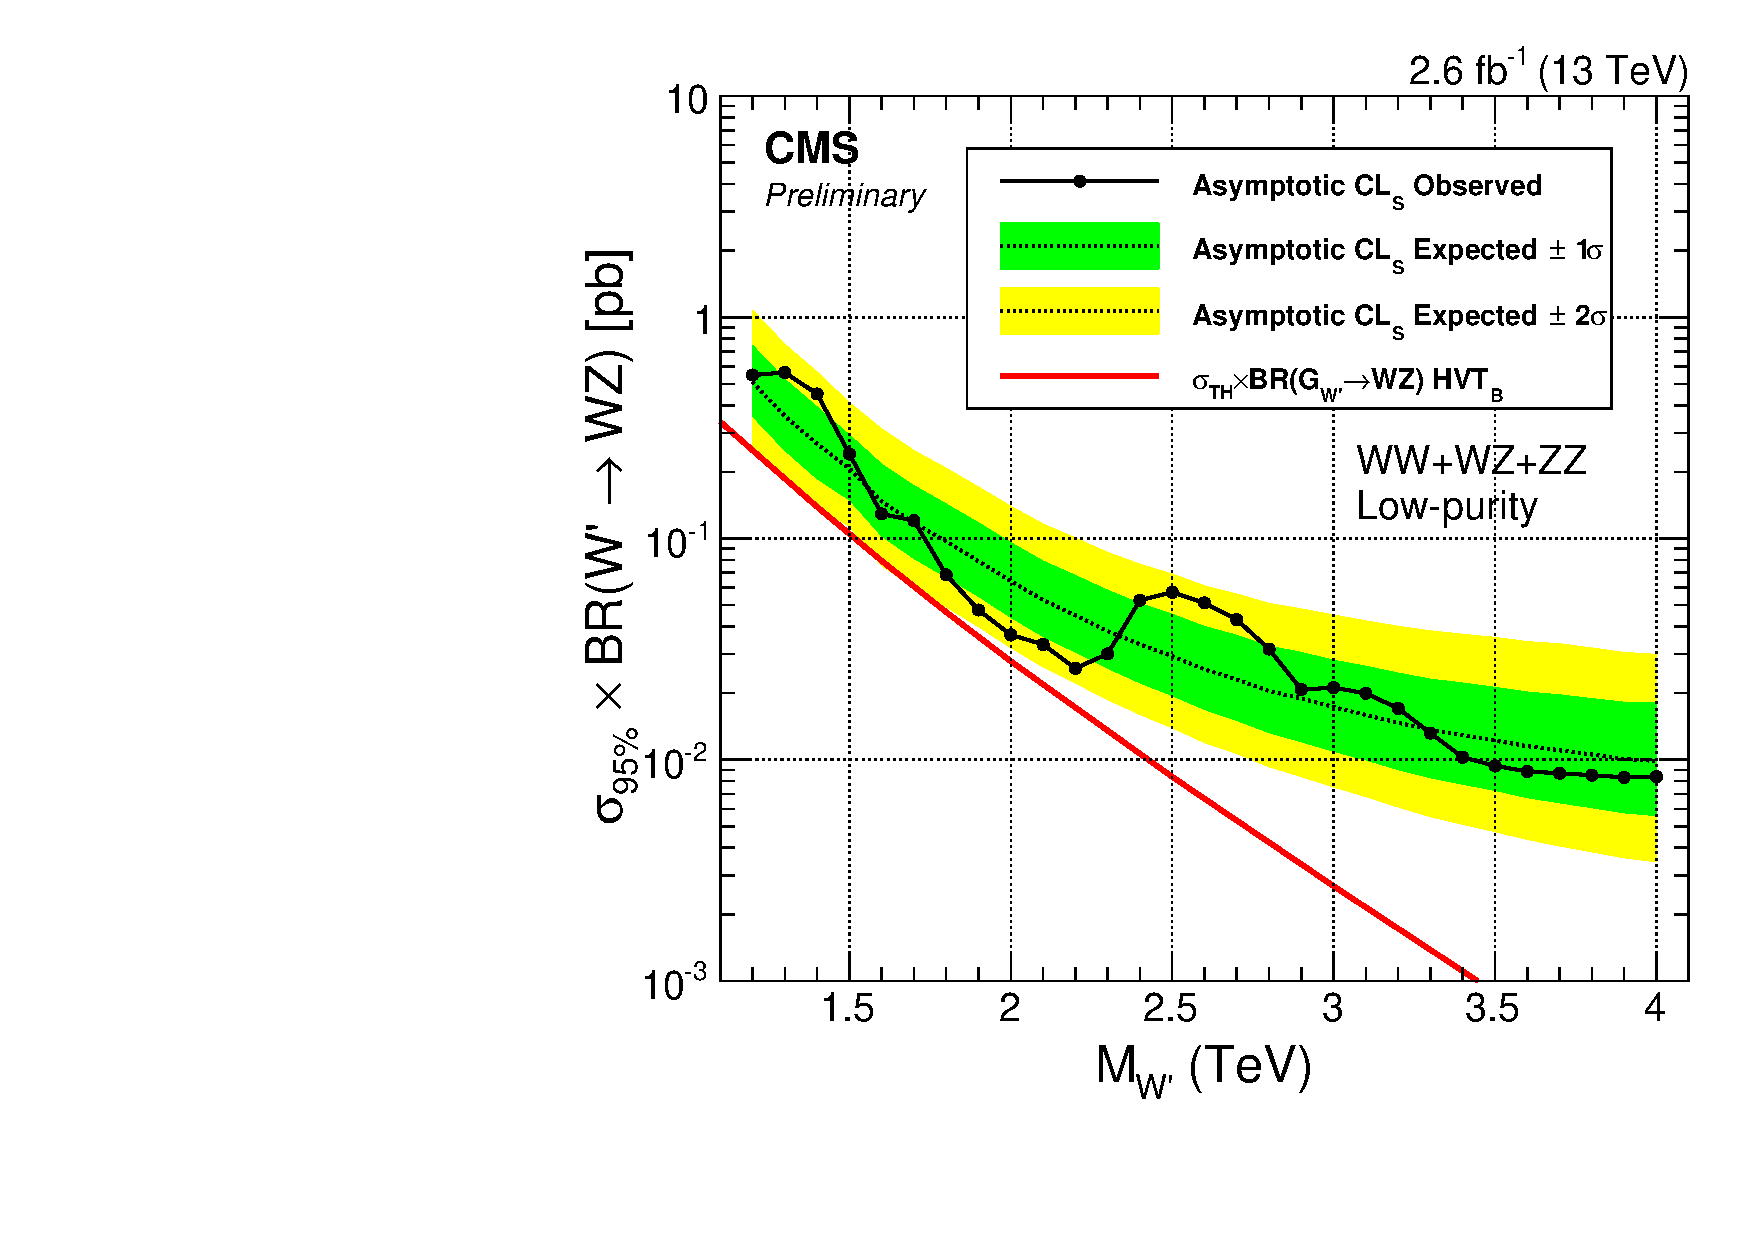
\includegraphics[width=0.327\textwidth]{figures/analysis/search1/AN-15-211/limits/brazilianFlag_WZ_VVLP_new_combined_purity_13TeV_wPDF.pdf}
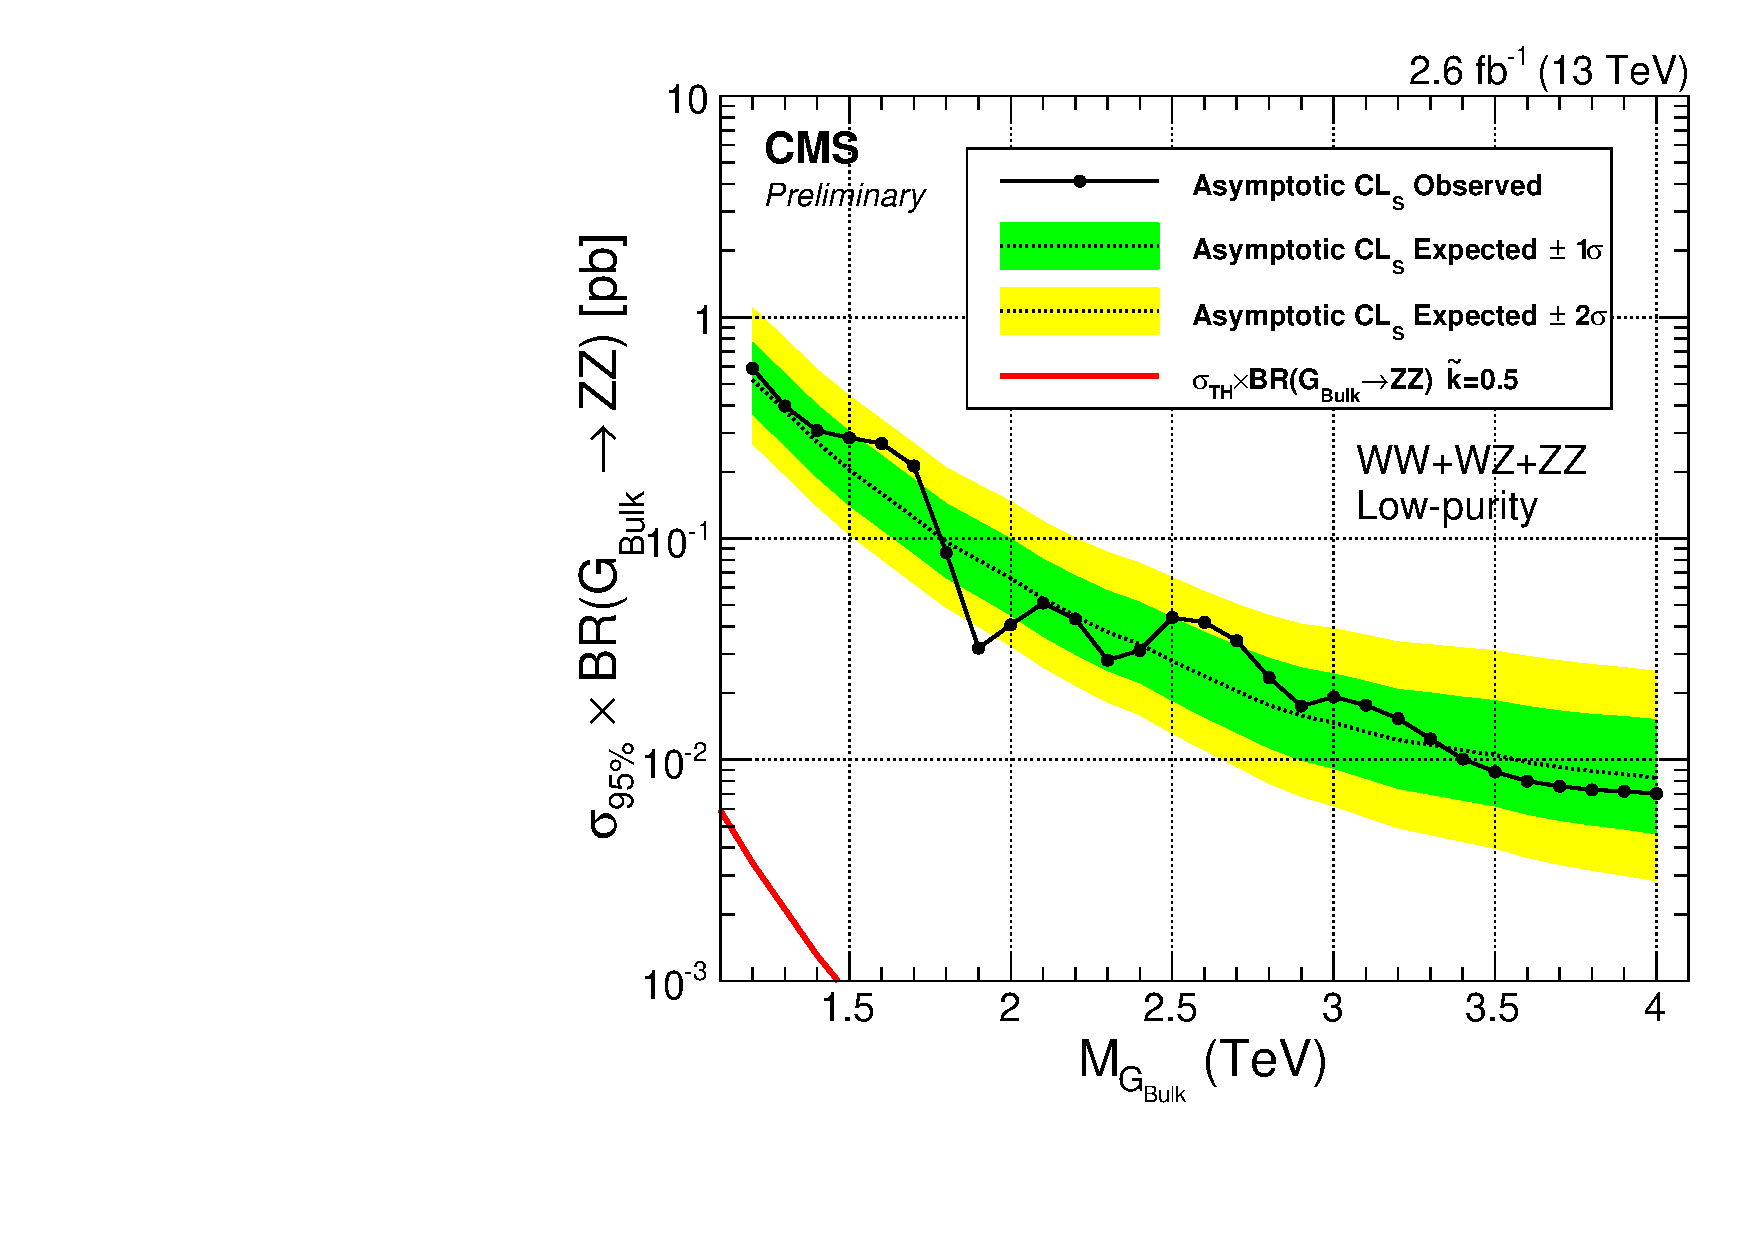
\includegraphics[width=0.327\textwidth]{figures/analysis/search1/AN-15-211/limits/brazilianFlag_BulkZZ_VVLP_new_combined_purity_13TeV_wPDF.pdf}\\
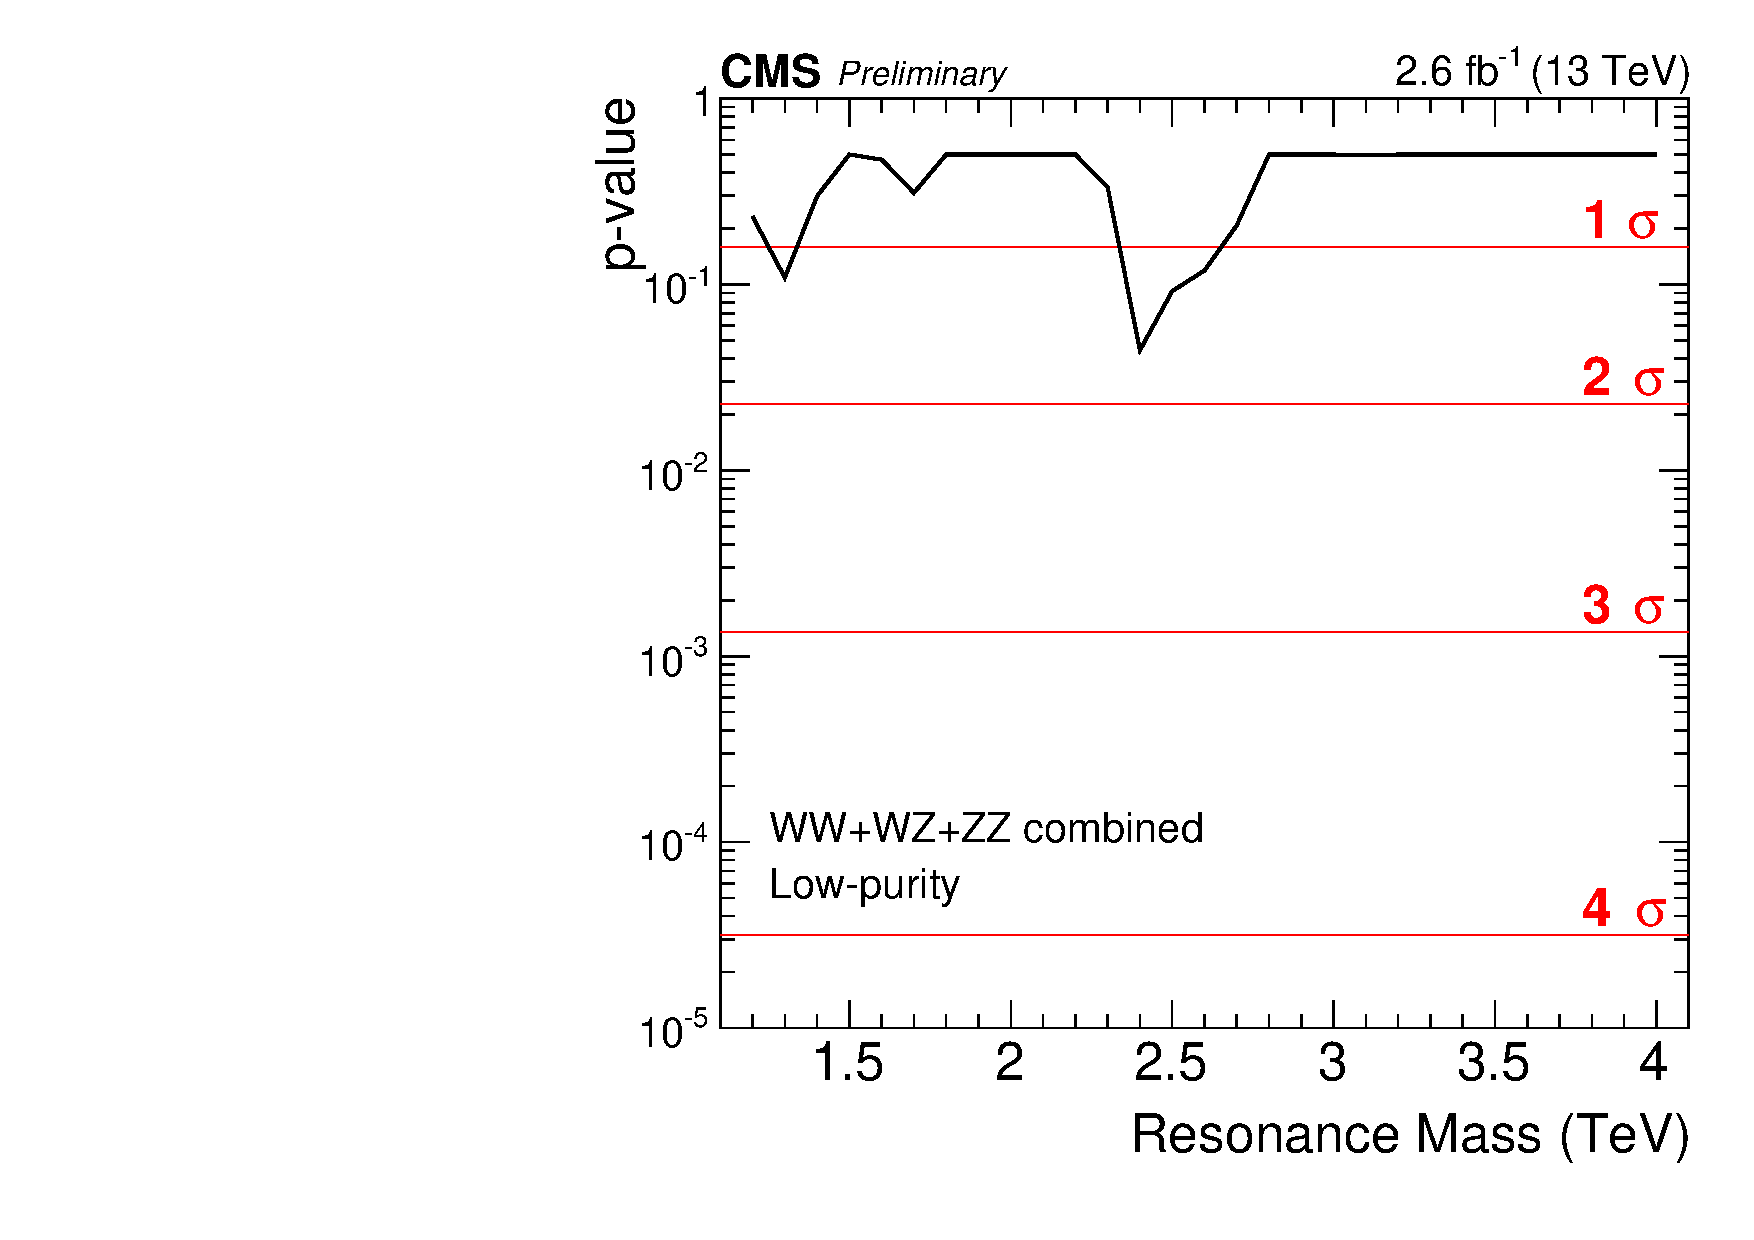
\includegraphics[width=0.327\textwidth]{figures/analysis/search1/AN-15-211/pvalues/pvalue_BulkWWinVVnew_low_purity.pdf}
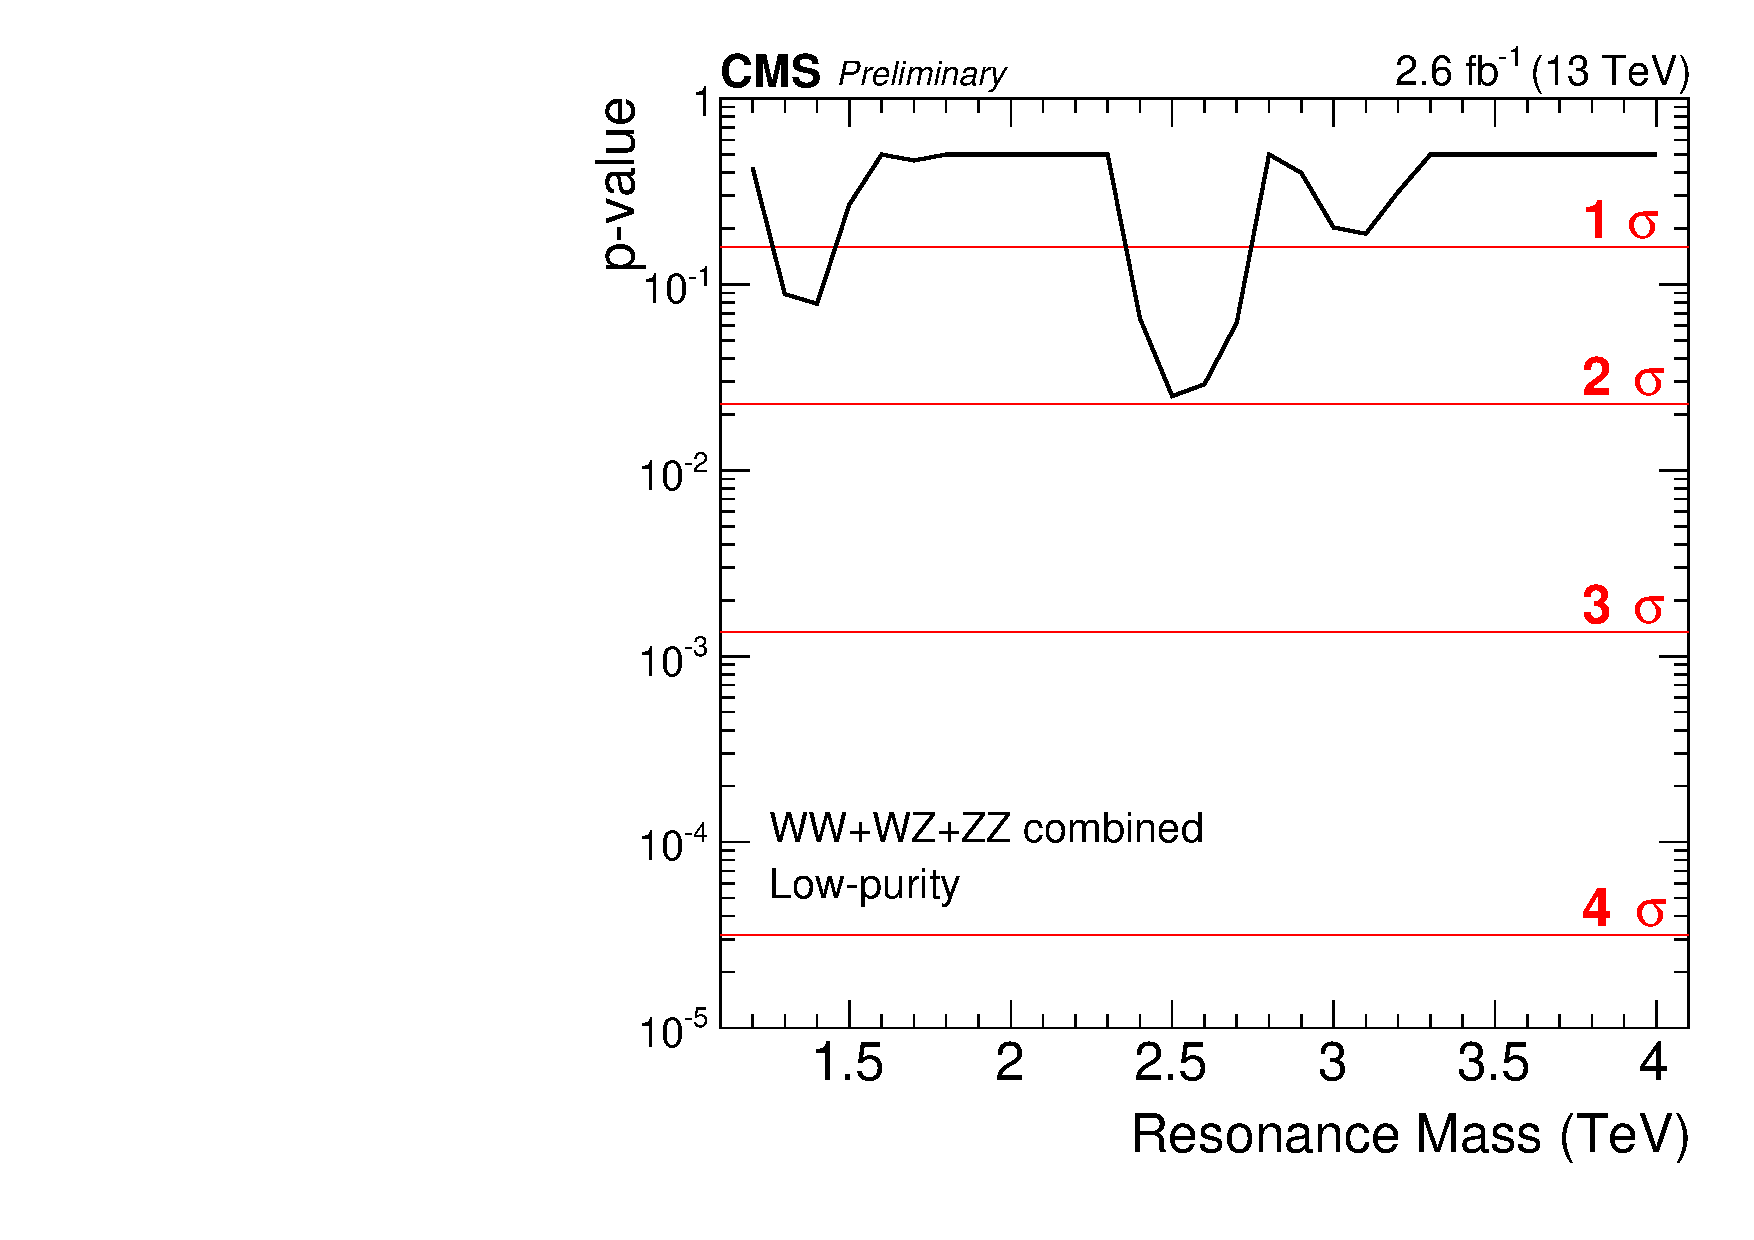
\includegraphics[width=0.327\textwidth]{figures/analysis/search1/AN-15-211/pvalues/pvalue_WZinVVnew_low_purity.pdf}
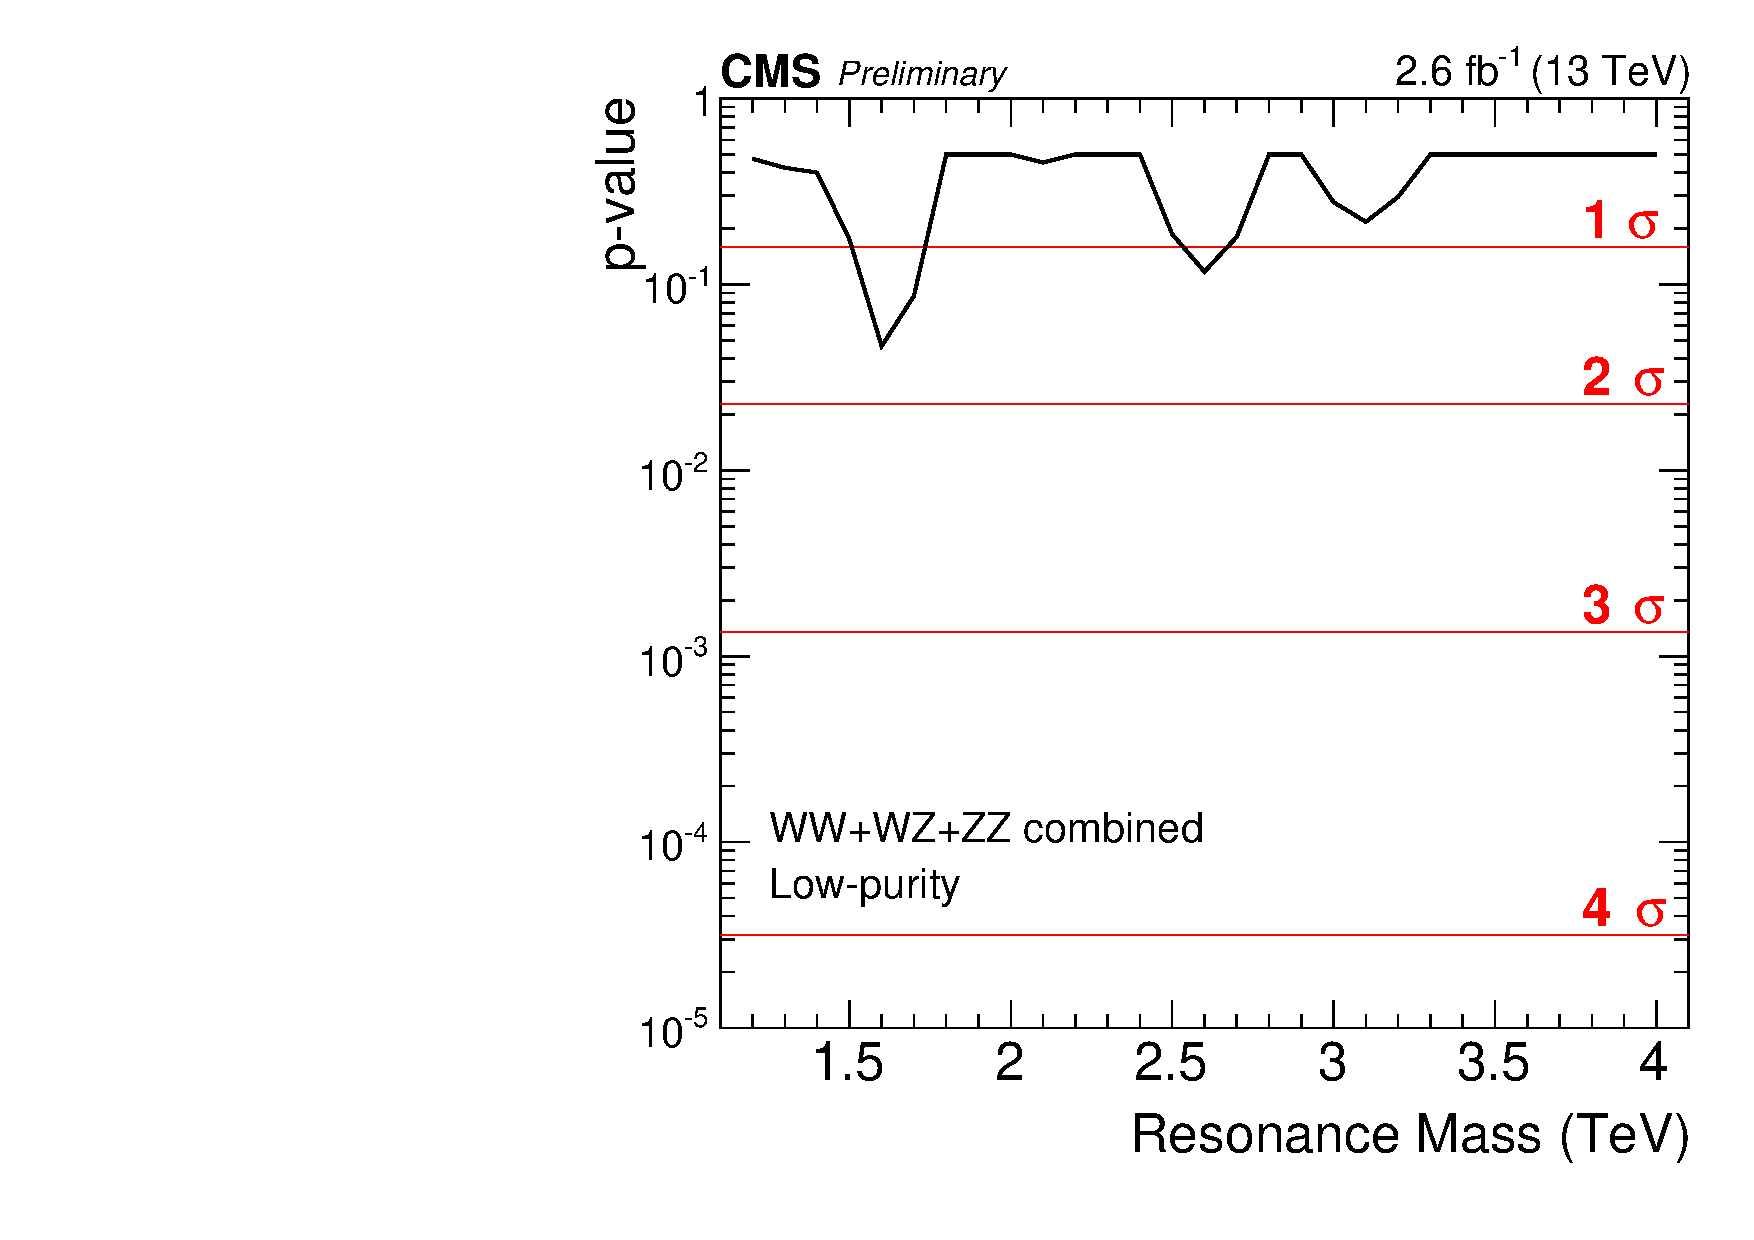
\includegraphics[width=0.327\textwidth]{figures/analysis/search1/AN-15-211/pvalues/pvalue_BulkZZinVVnew_low_purity.pdf}
\caption{Expected and observed limits at 95\% CL and corresponding p-values obtained in the low purity category using 2.6 $\textrm{fb}^{-1}$ of CMS data. Here for a Bulk $G\rightarrow WW$ (left), $W'\rightarrow WZ$ (middle) and $G\rightarrow ZZ$ (right) signal.}
\label{fig:app:Limits_LP}
\end{figure}
\begin{figure}[h!]
\centering
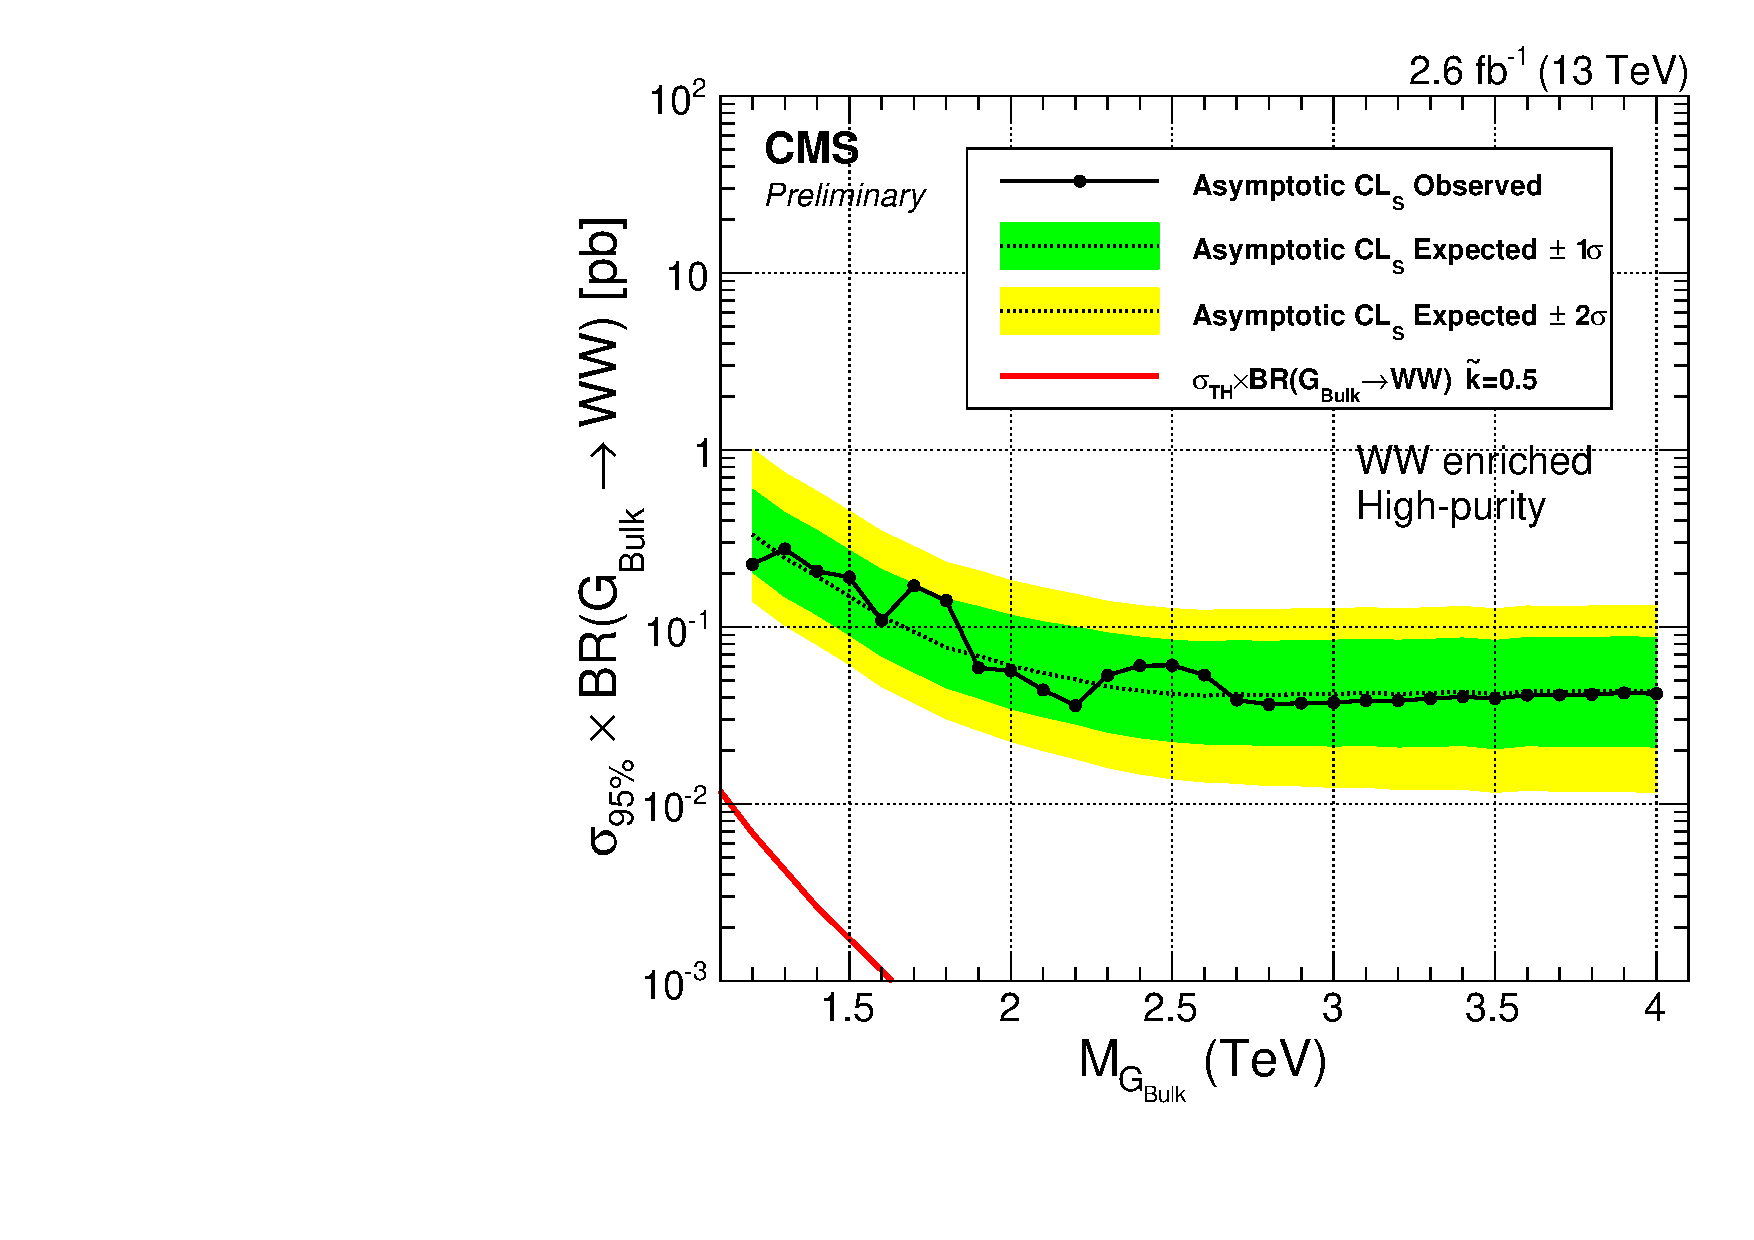
\includegraphics[width=0.327\textwidth]{figures/analysis/search1/AN-15-211/limits/brazilianFlag_BulkWW_WWHP_13TeV_wPDF.pdf}
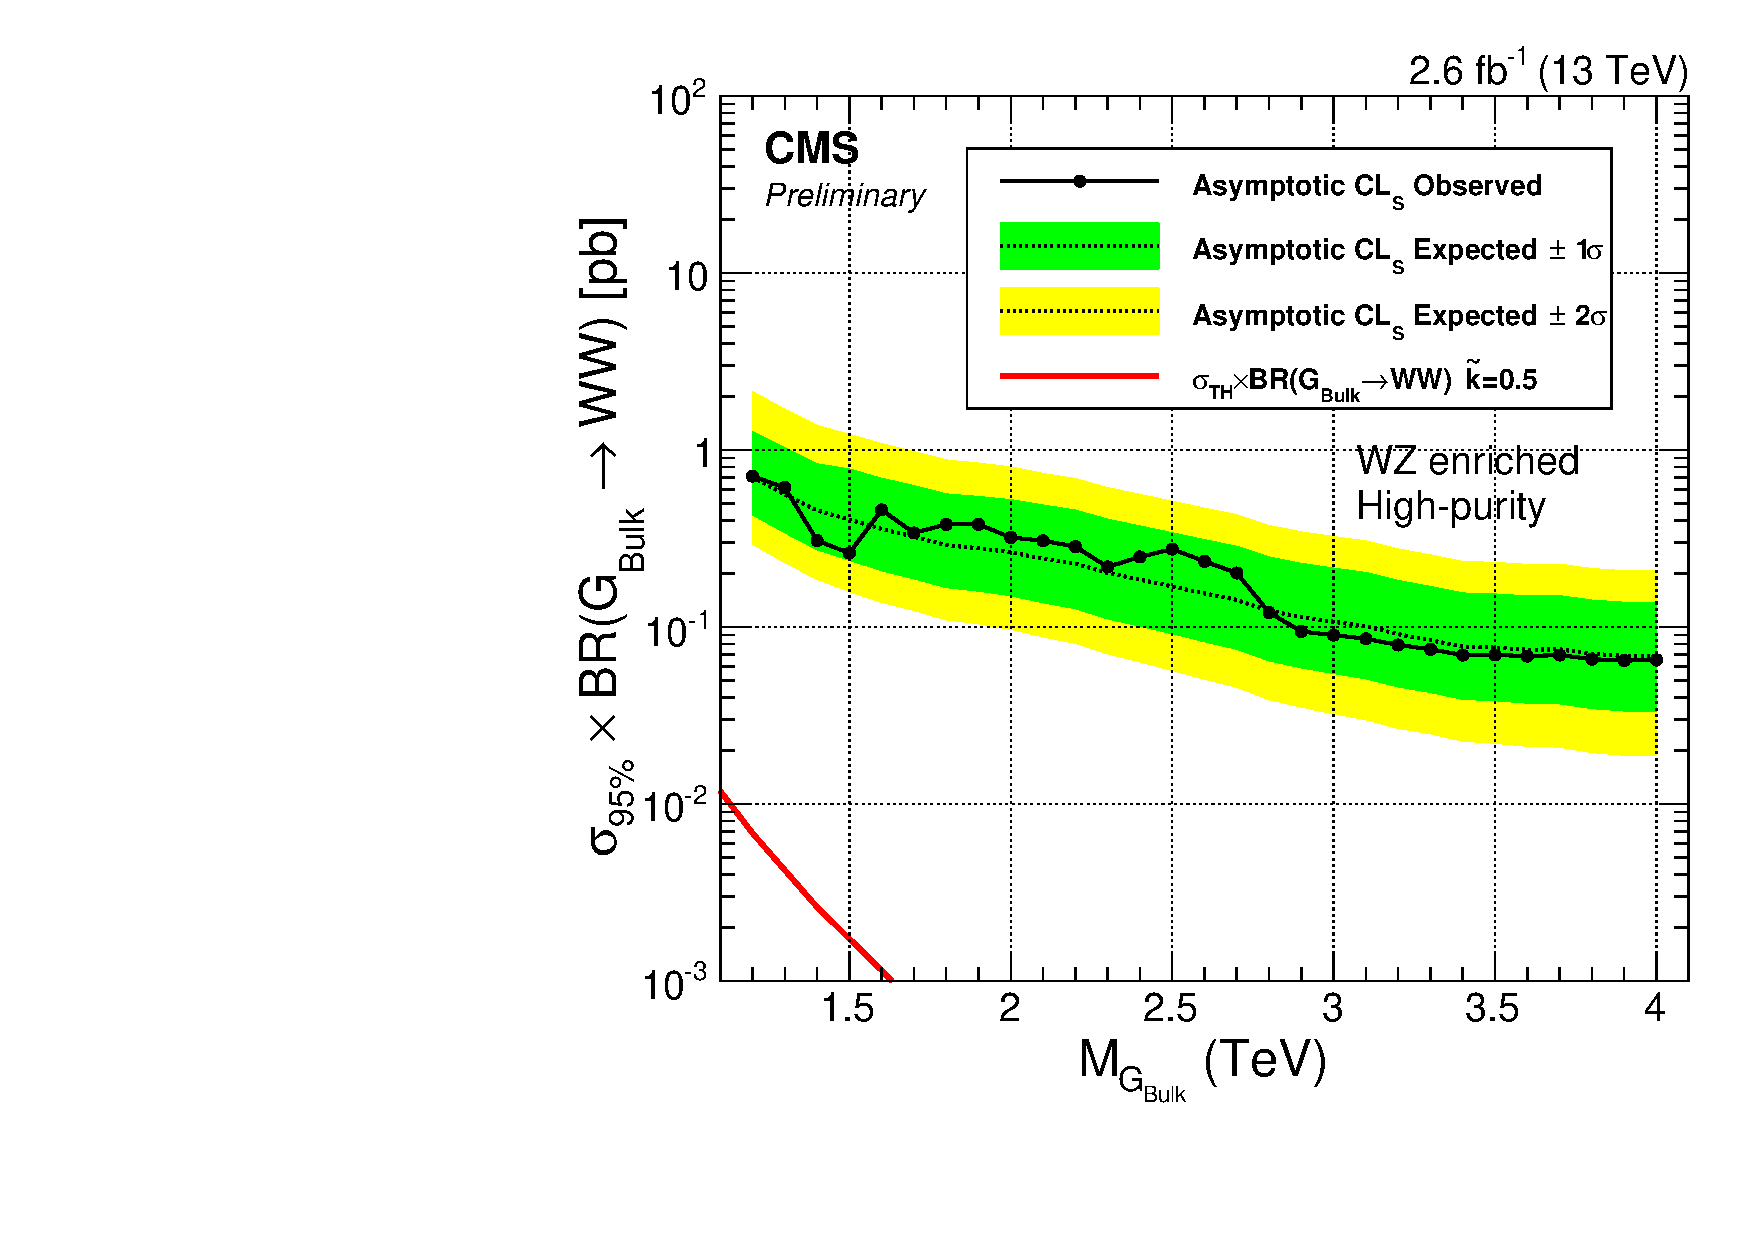
\includegraphics[width=0.327\textwidth]{figures/analysis/search1/AN-15-211/limits/brazilianFlag_BulkWW_WZHP_13TeV_wPDF.pdf}
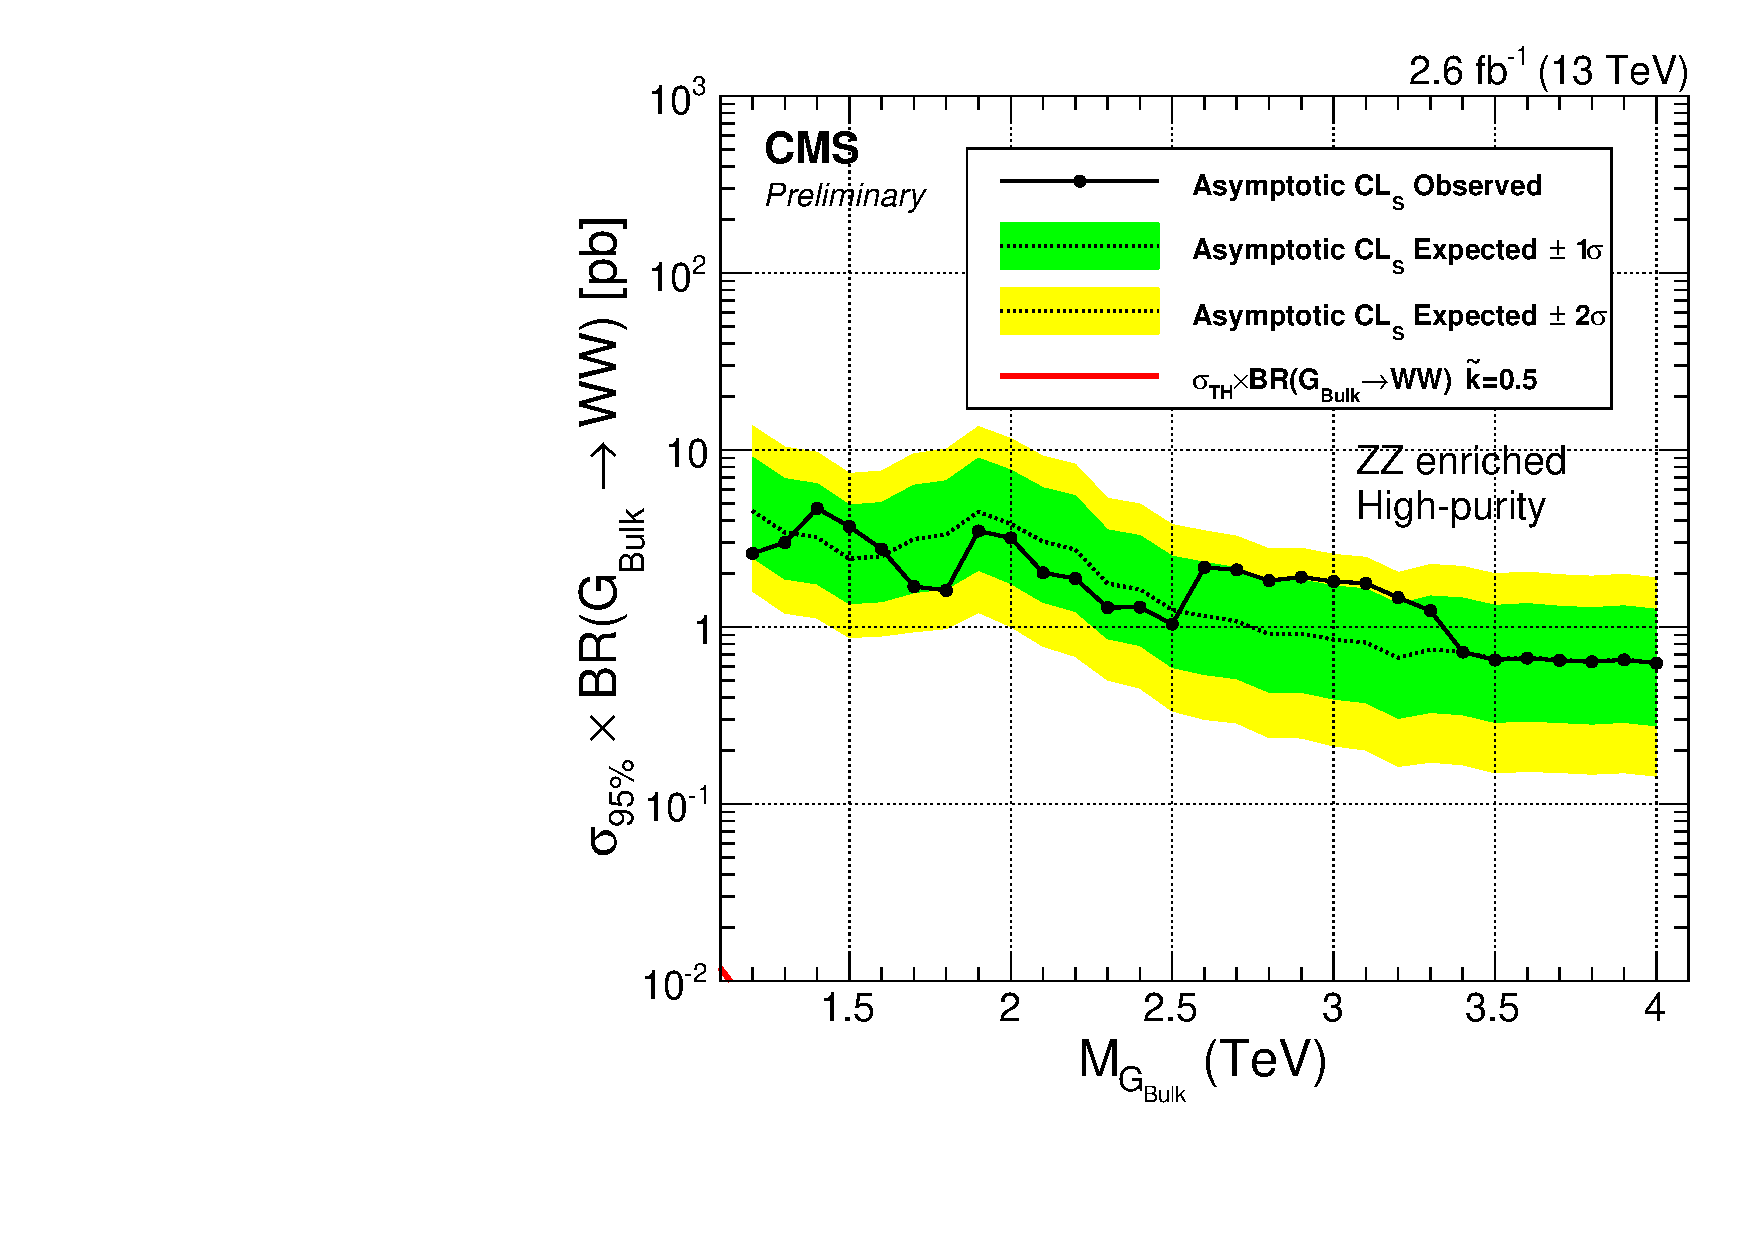
\includegraphics[width=0.327\textwidth]{figures/analysis/search1/AN-15-211/limits/brazilianFlag_BulkWW_ZZHP_13TeV_wPDF.pdf}\\
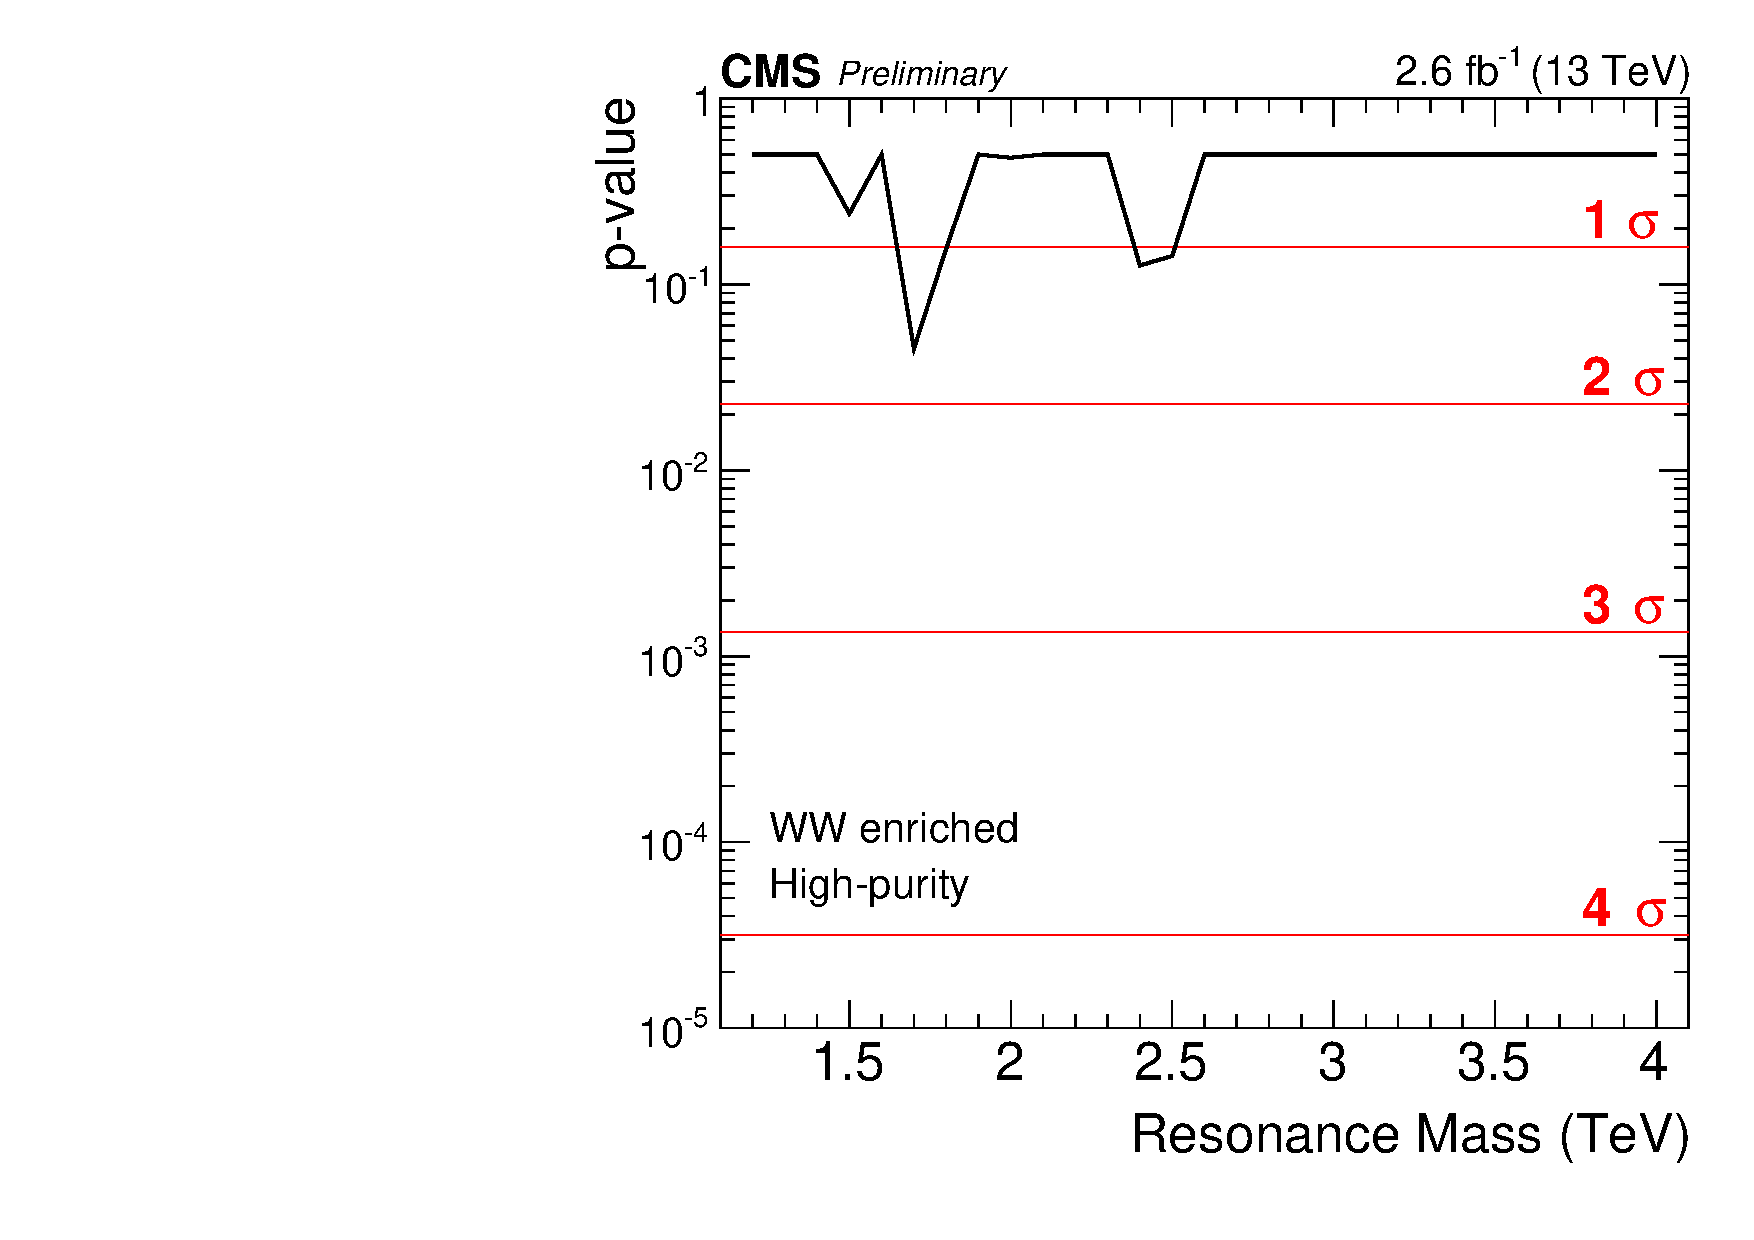
\includegraphics[width=0.327\textwidth]{figures/analysis/search1/AN-15-211/pvalues/pvalue_BulkWWinWW_high_purity.pdf}
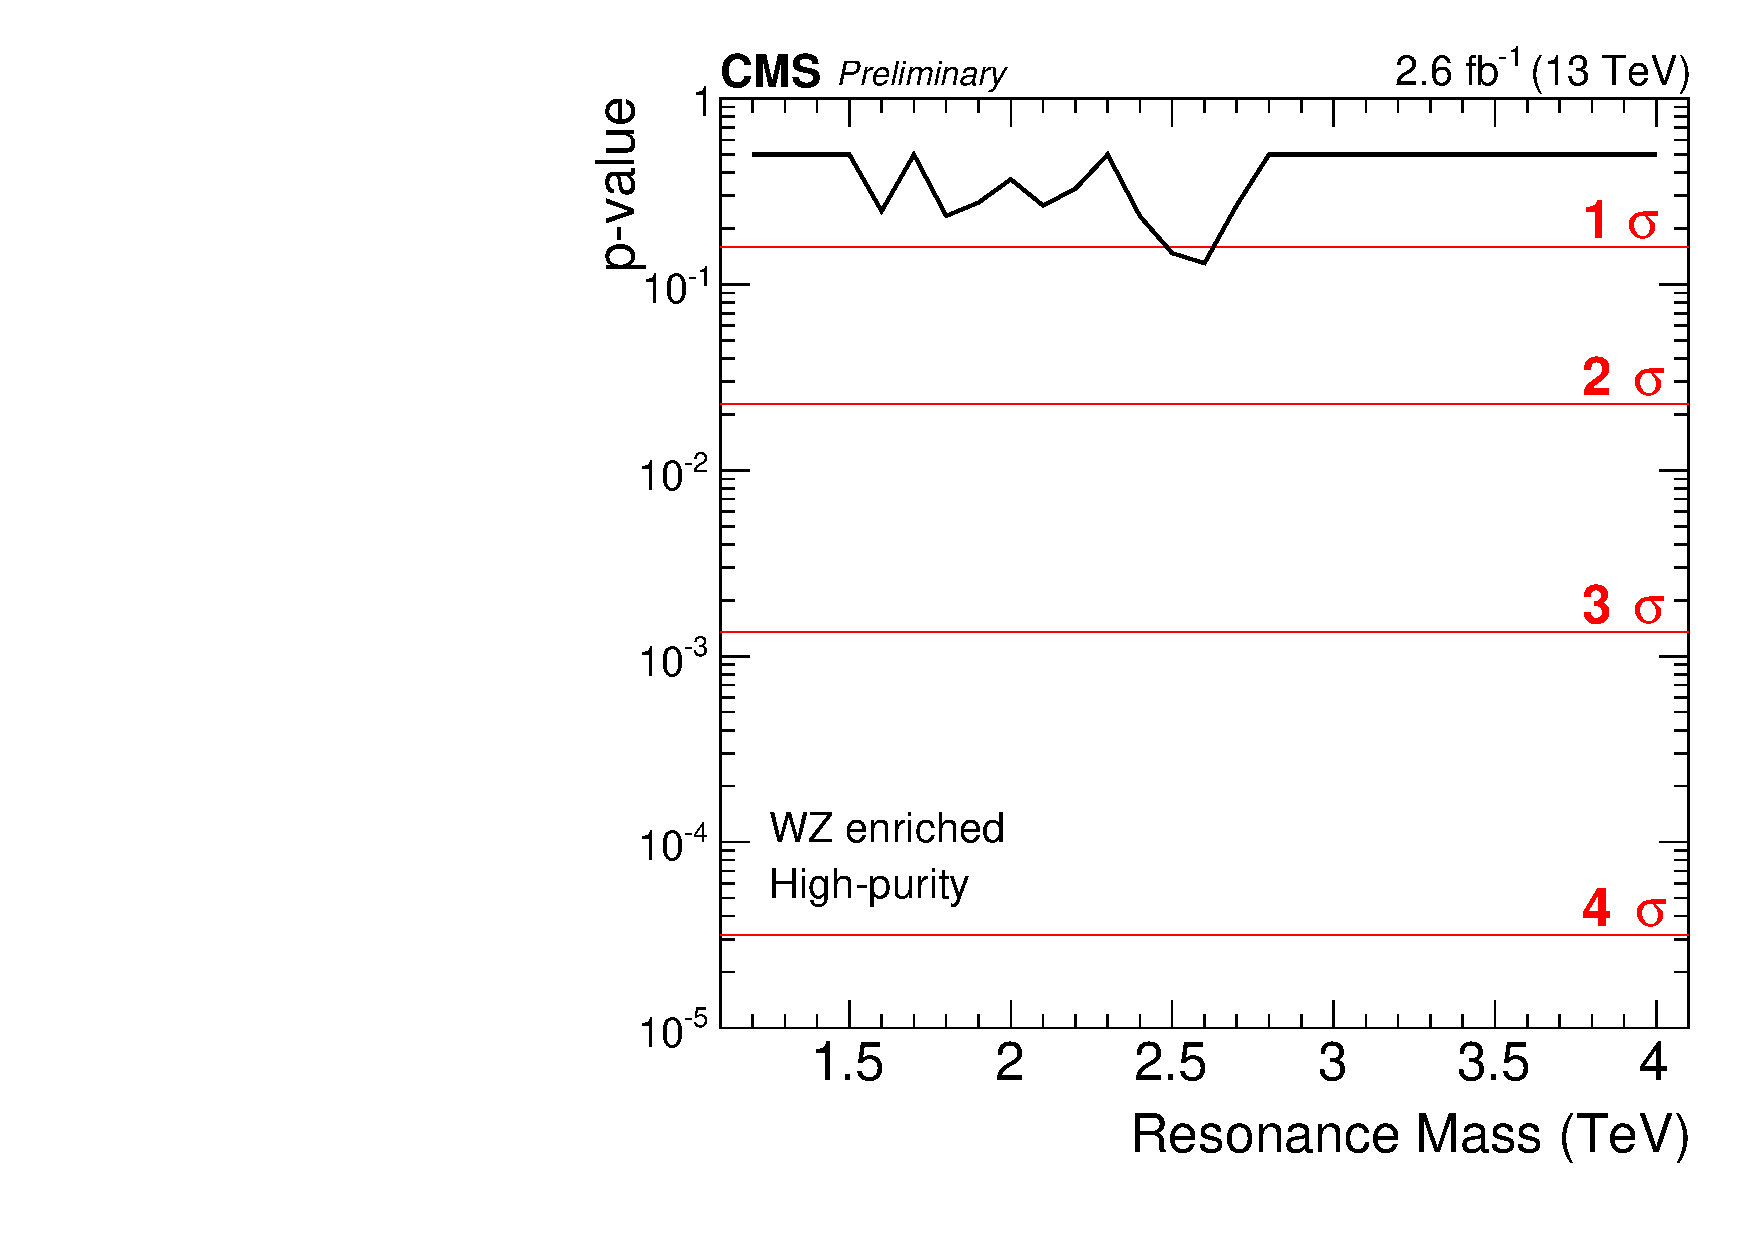
\includegraphics[width=0.327\textwidth]{figures/analysis/search1/AN-15-211/pvalues/pvalue_BulkWWinWZ_high_purity.pdf}
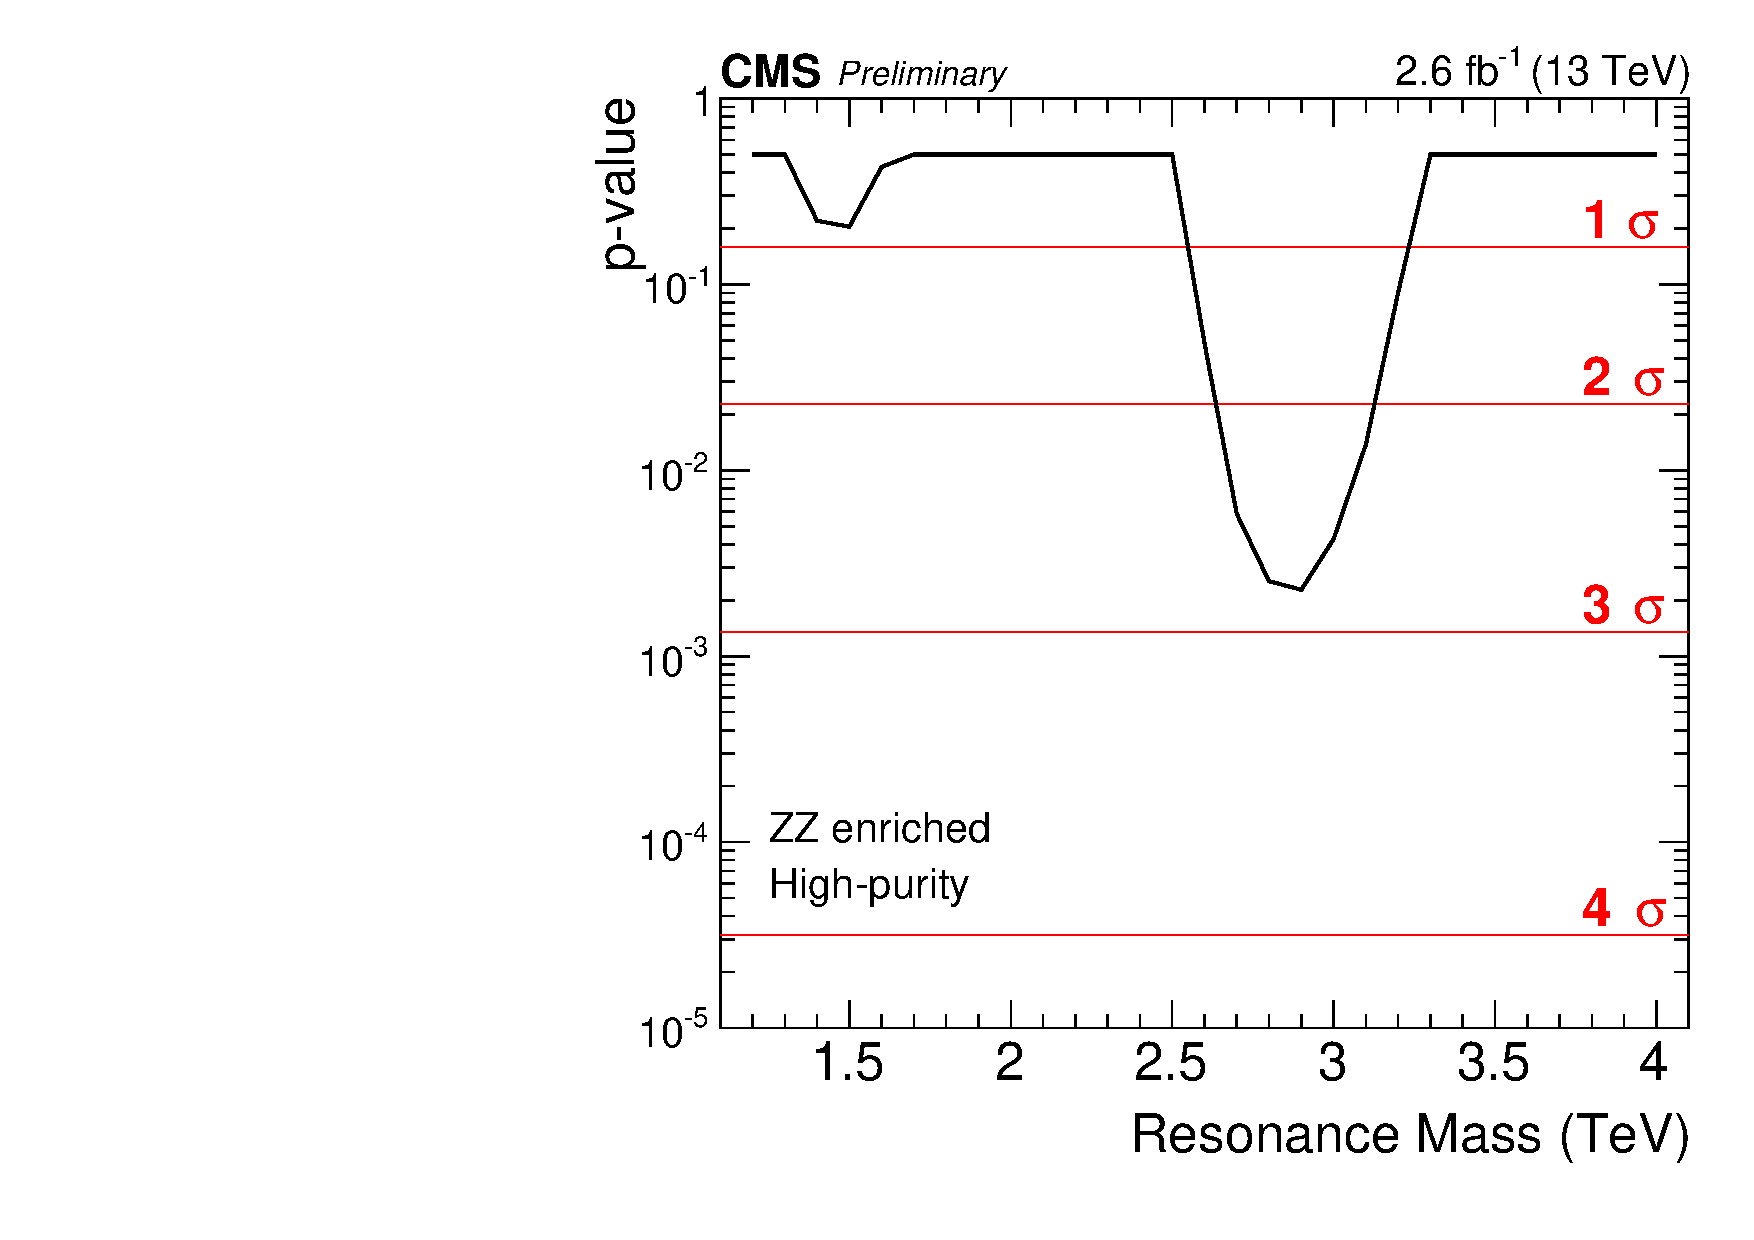
\includegraphics[width=0.327\textwidth]{figures/analysis/search1/AN-15-211/pvalues/pvalue_BulkWWinZZ_high_purity.pdf}
\caption{Expected and observed limits at 95\% CL and corresponding p-values obtained for the different mass categories using 2.6 $\textrm{fb}^{-1}$ of CMS data. Here for a Bulk $G\rightarrow WW$ signal in the HP category}
\label{fig:app:Limits_HPBulkWW}
\end{figure}
\begin{figure}[h!]
\centering
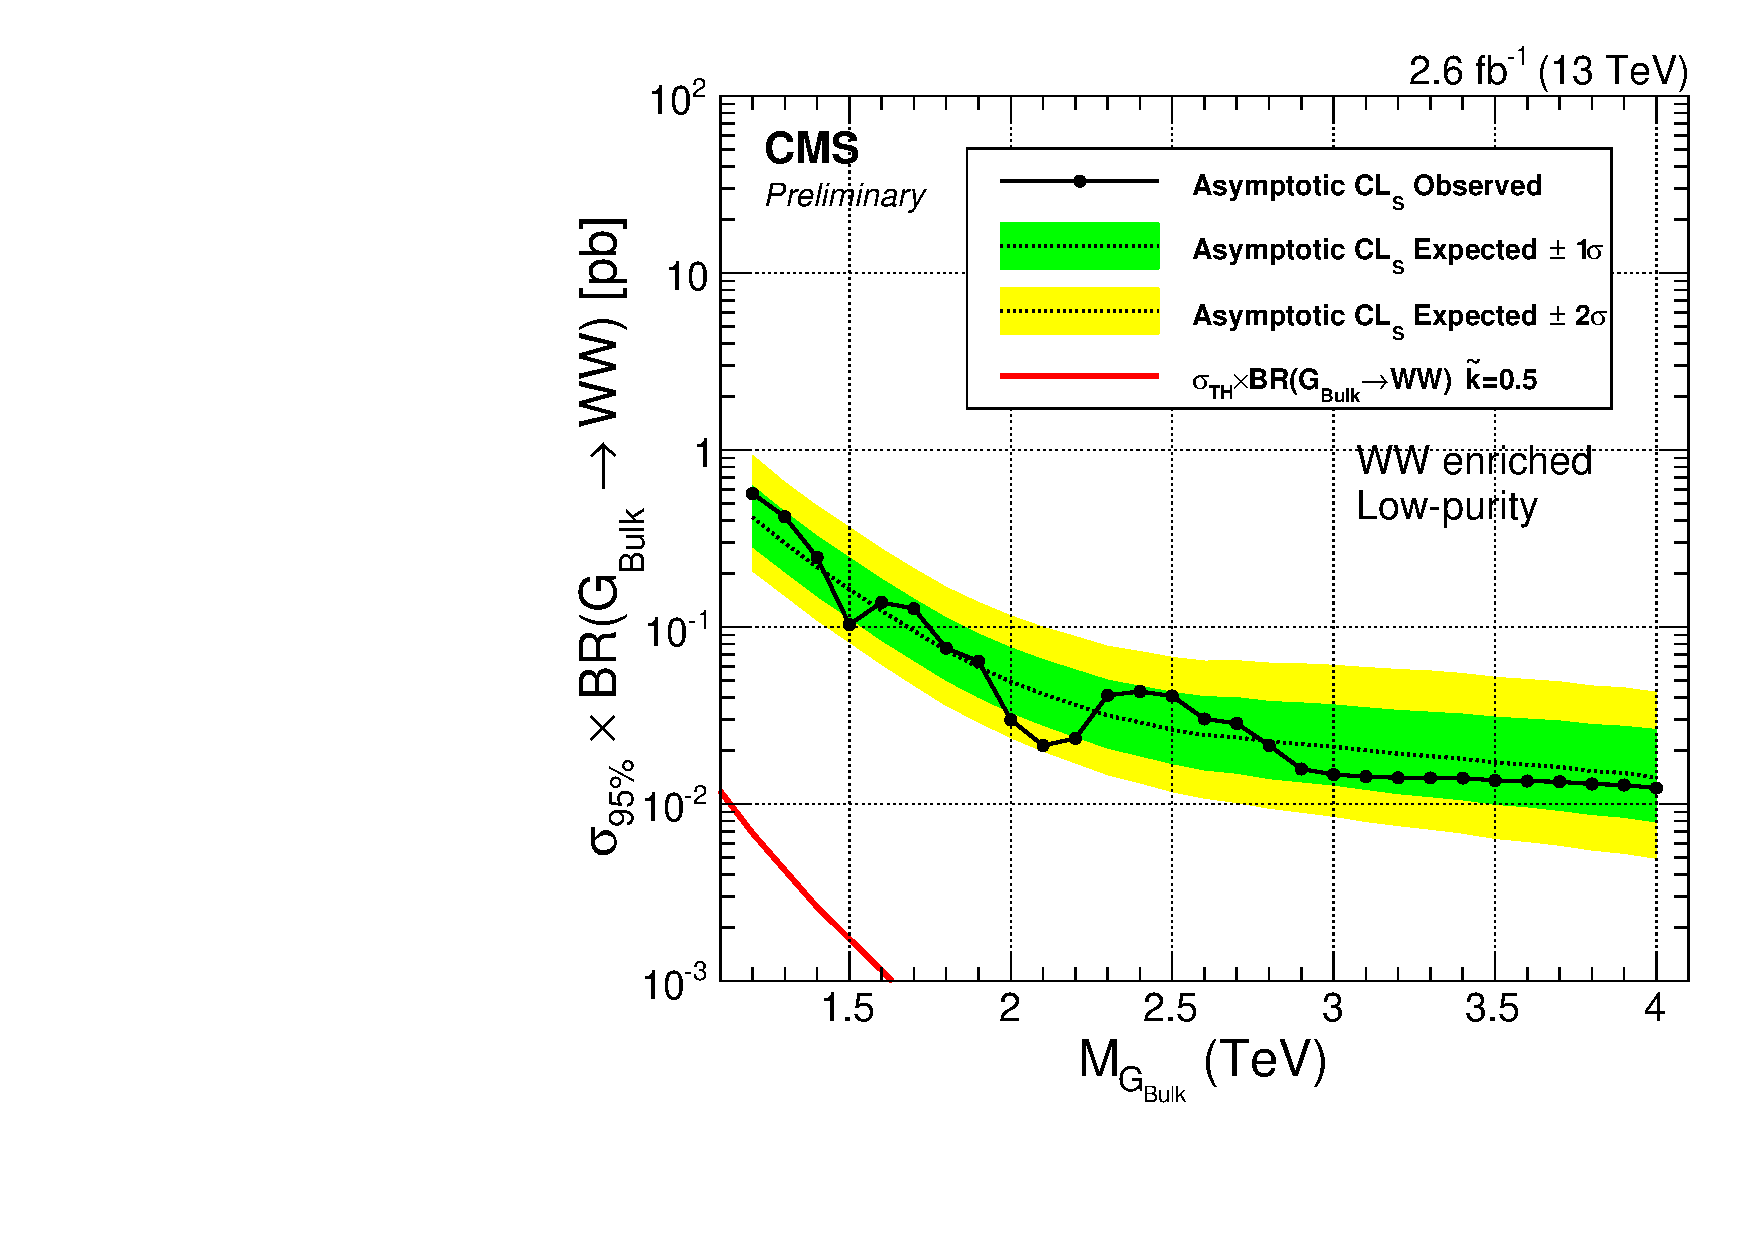
\includegraphics[width=0.327\textwidth]{figures/analysis/search1/AN-15-211/limits/brazilianFlag_BulkWW_WWLP_13TeV_wPDF.pdf}
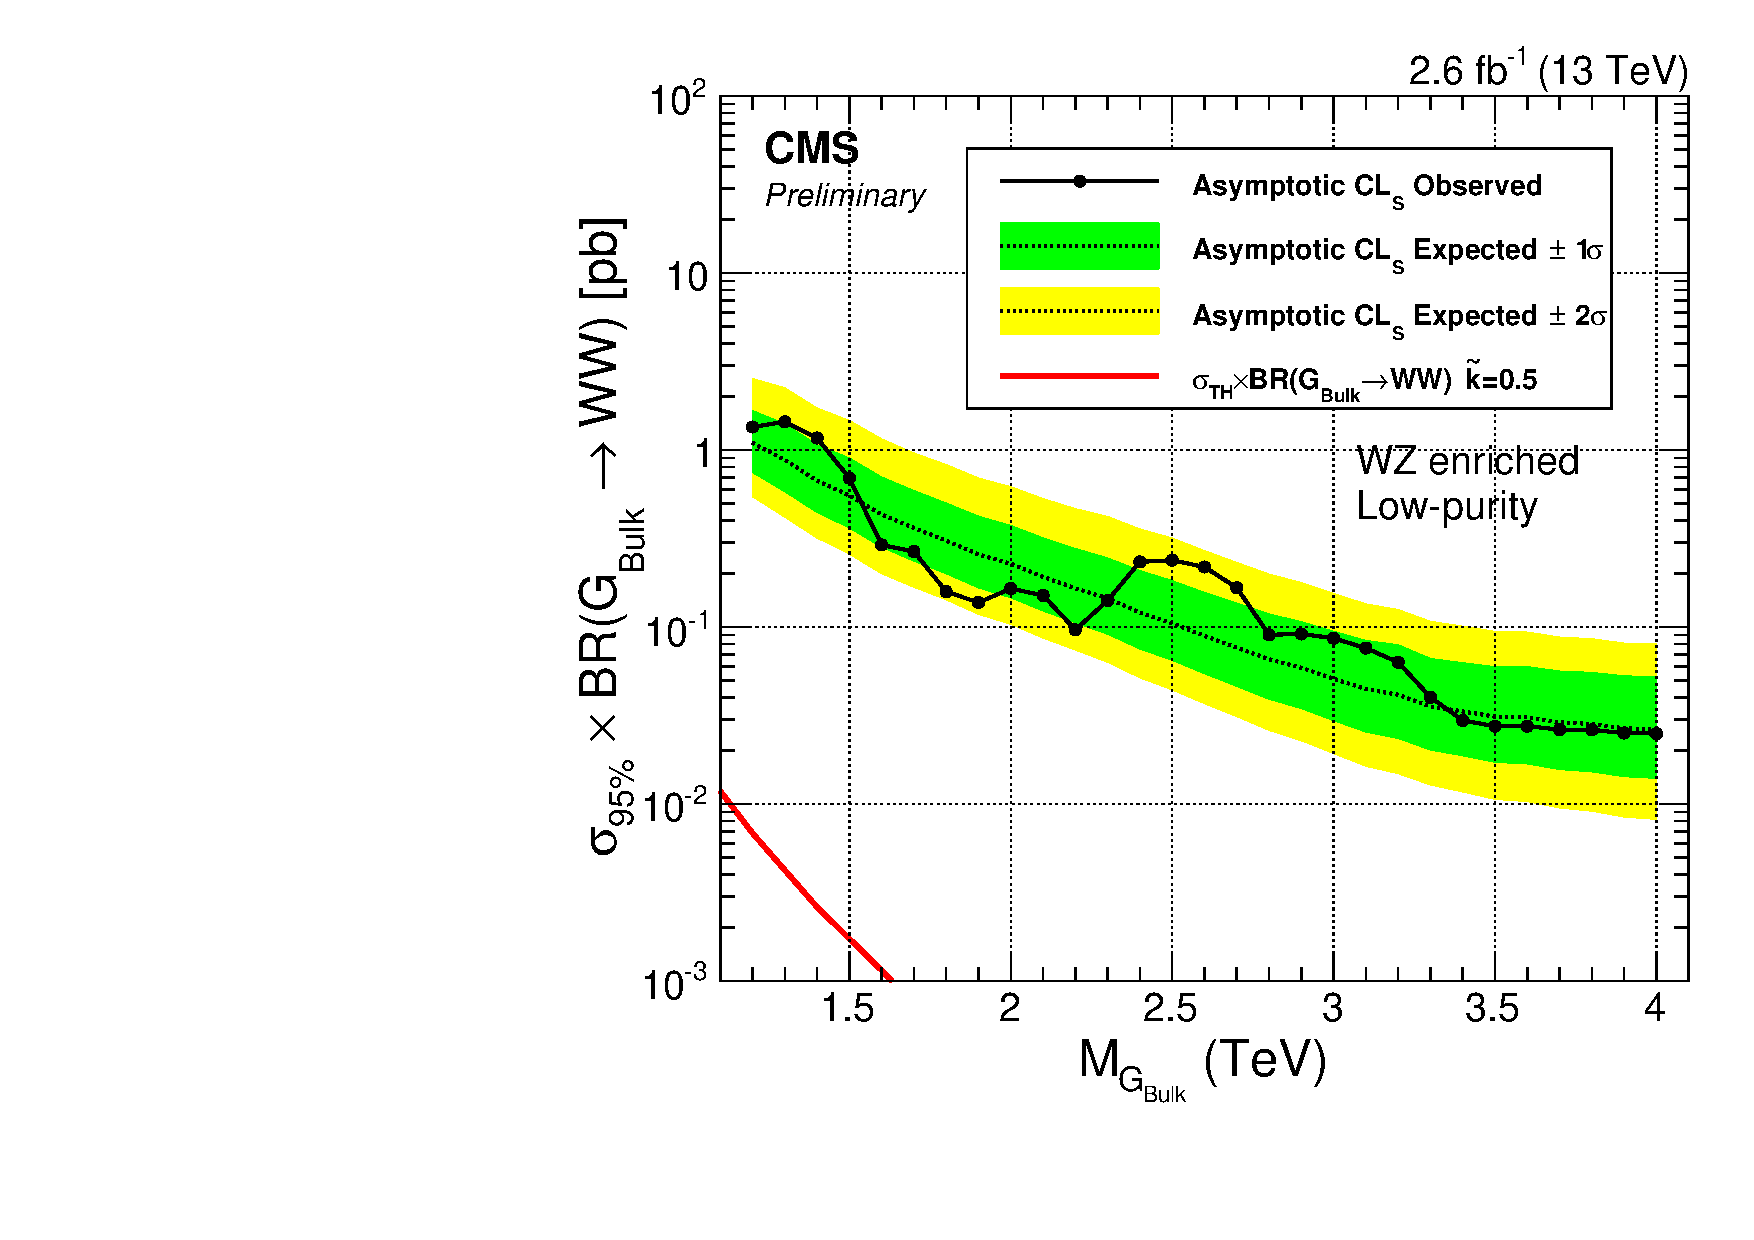
\includegraphics[width=0.327\textwidth]{figures/analysis/search1/AN-15-211/limits/brazilianFlag_BulkWW_WZLP_13TeV_wPDF.pdf}
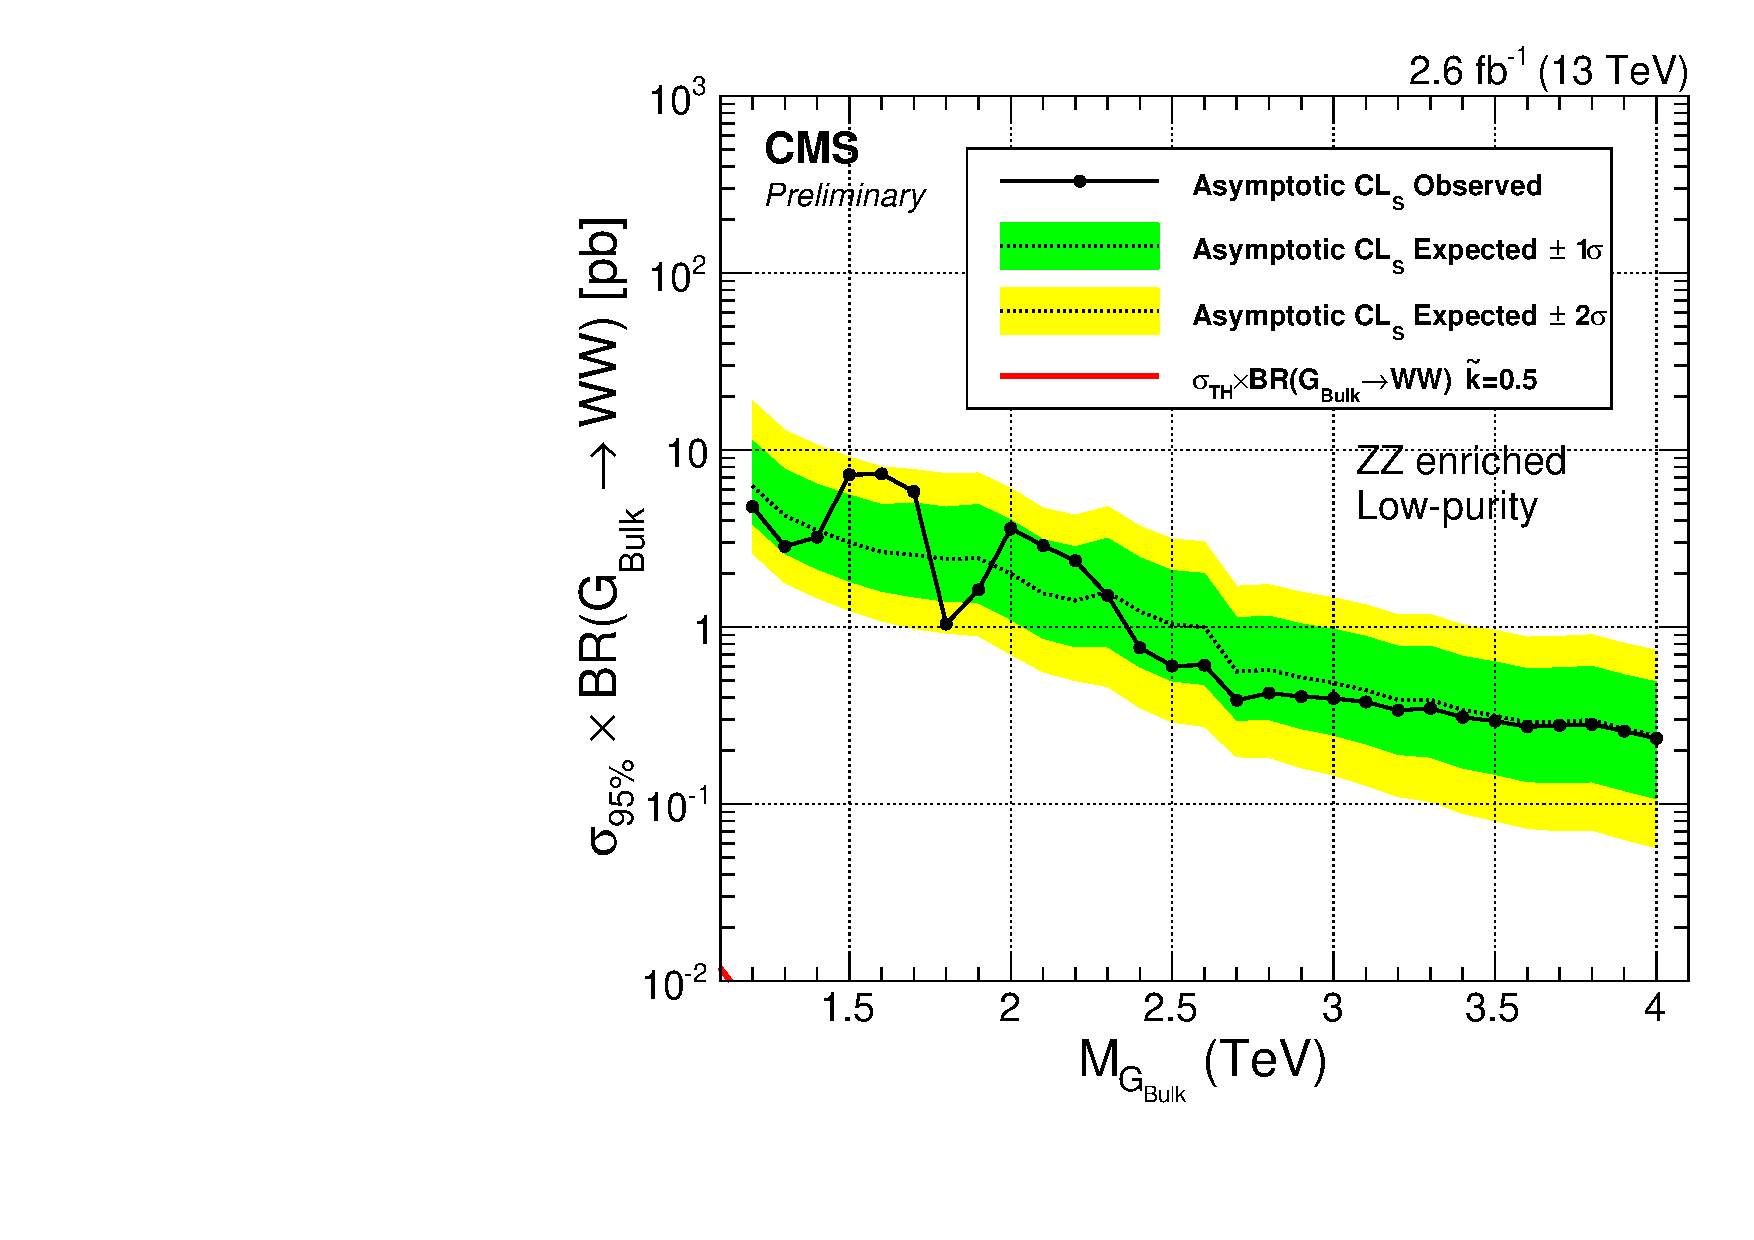
\includegraphics[width=0.327\textwidth]{figures/analysis/search1/AN-15-211/limits/brazilianFlag_BulkWW_ZZLP_13TeV_wPDF.pdf}\\
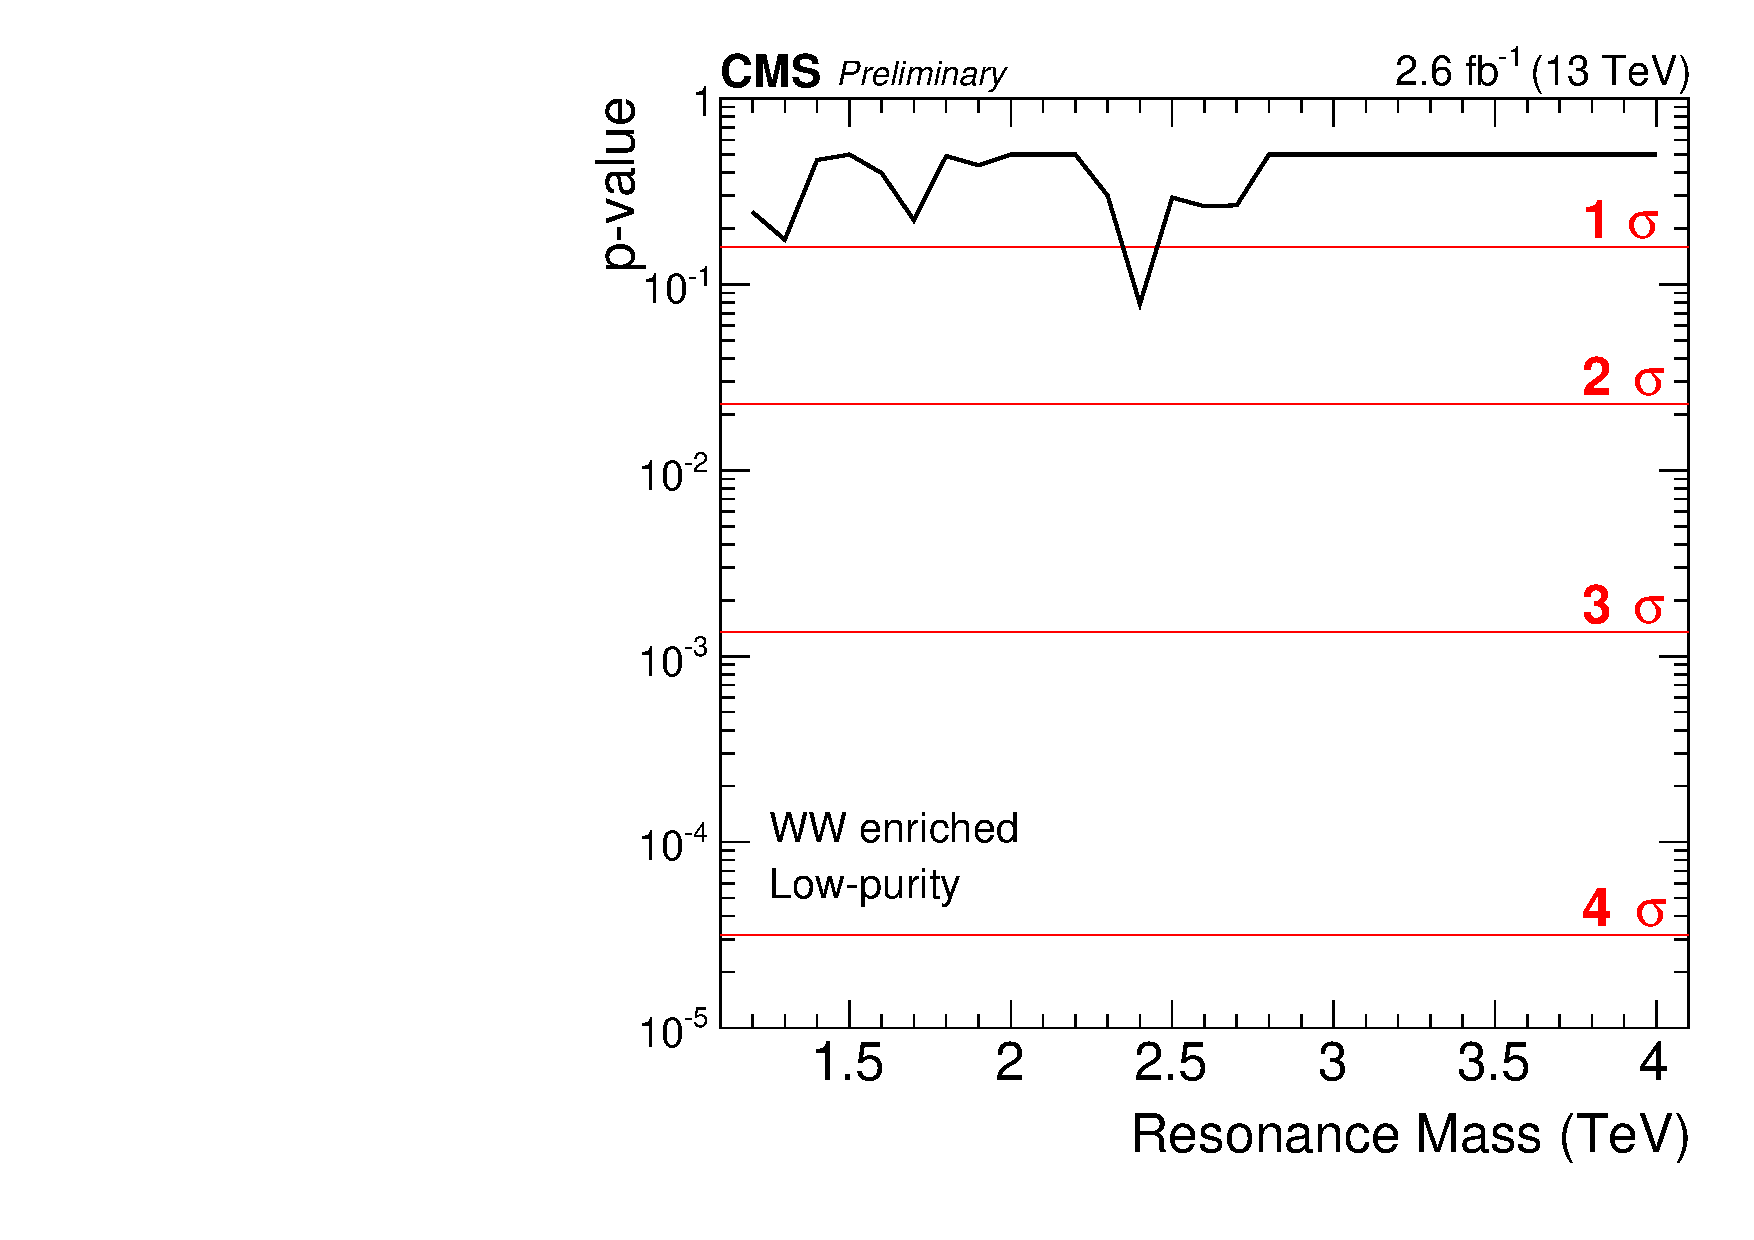
\includegraphics[width=0.327\textwidth]{figures/analysis/search1/AN-15-211/pvalues/pvalue_BulkWWinWW_low_purity.pdf}
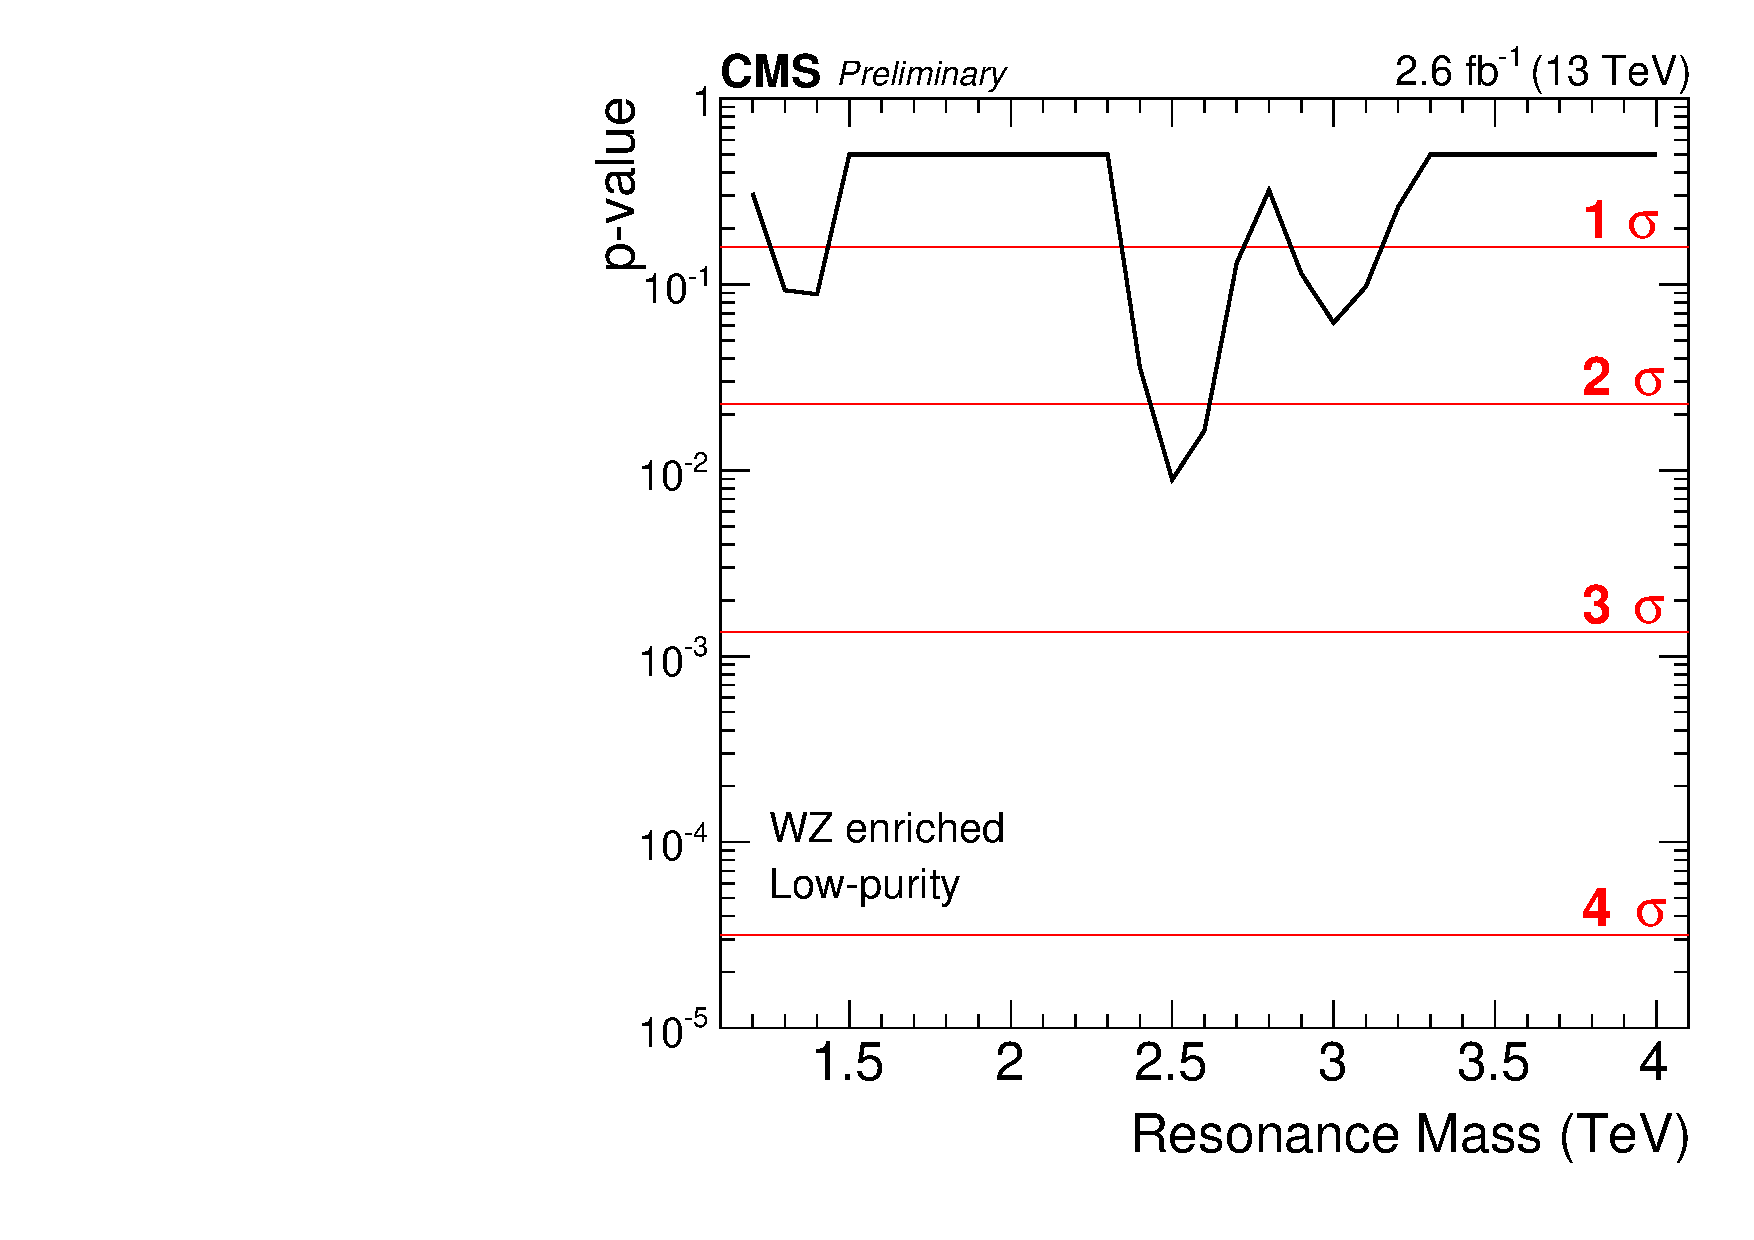
\includegraphics[width=0.327\textwidth]{figures/analysis/search1/AN-15-211/pvalues/pvalue_BulkWWinWZ_low_purity.pdf}
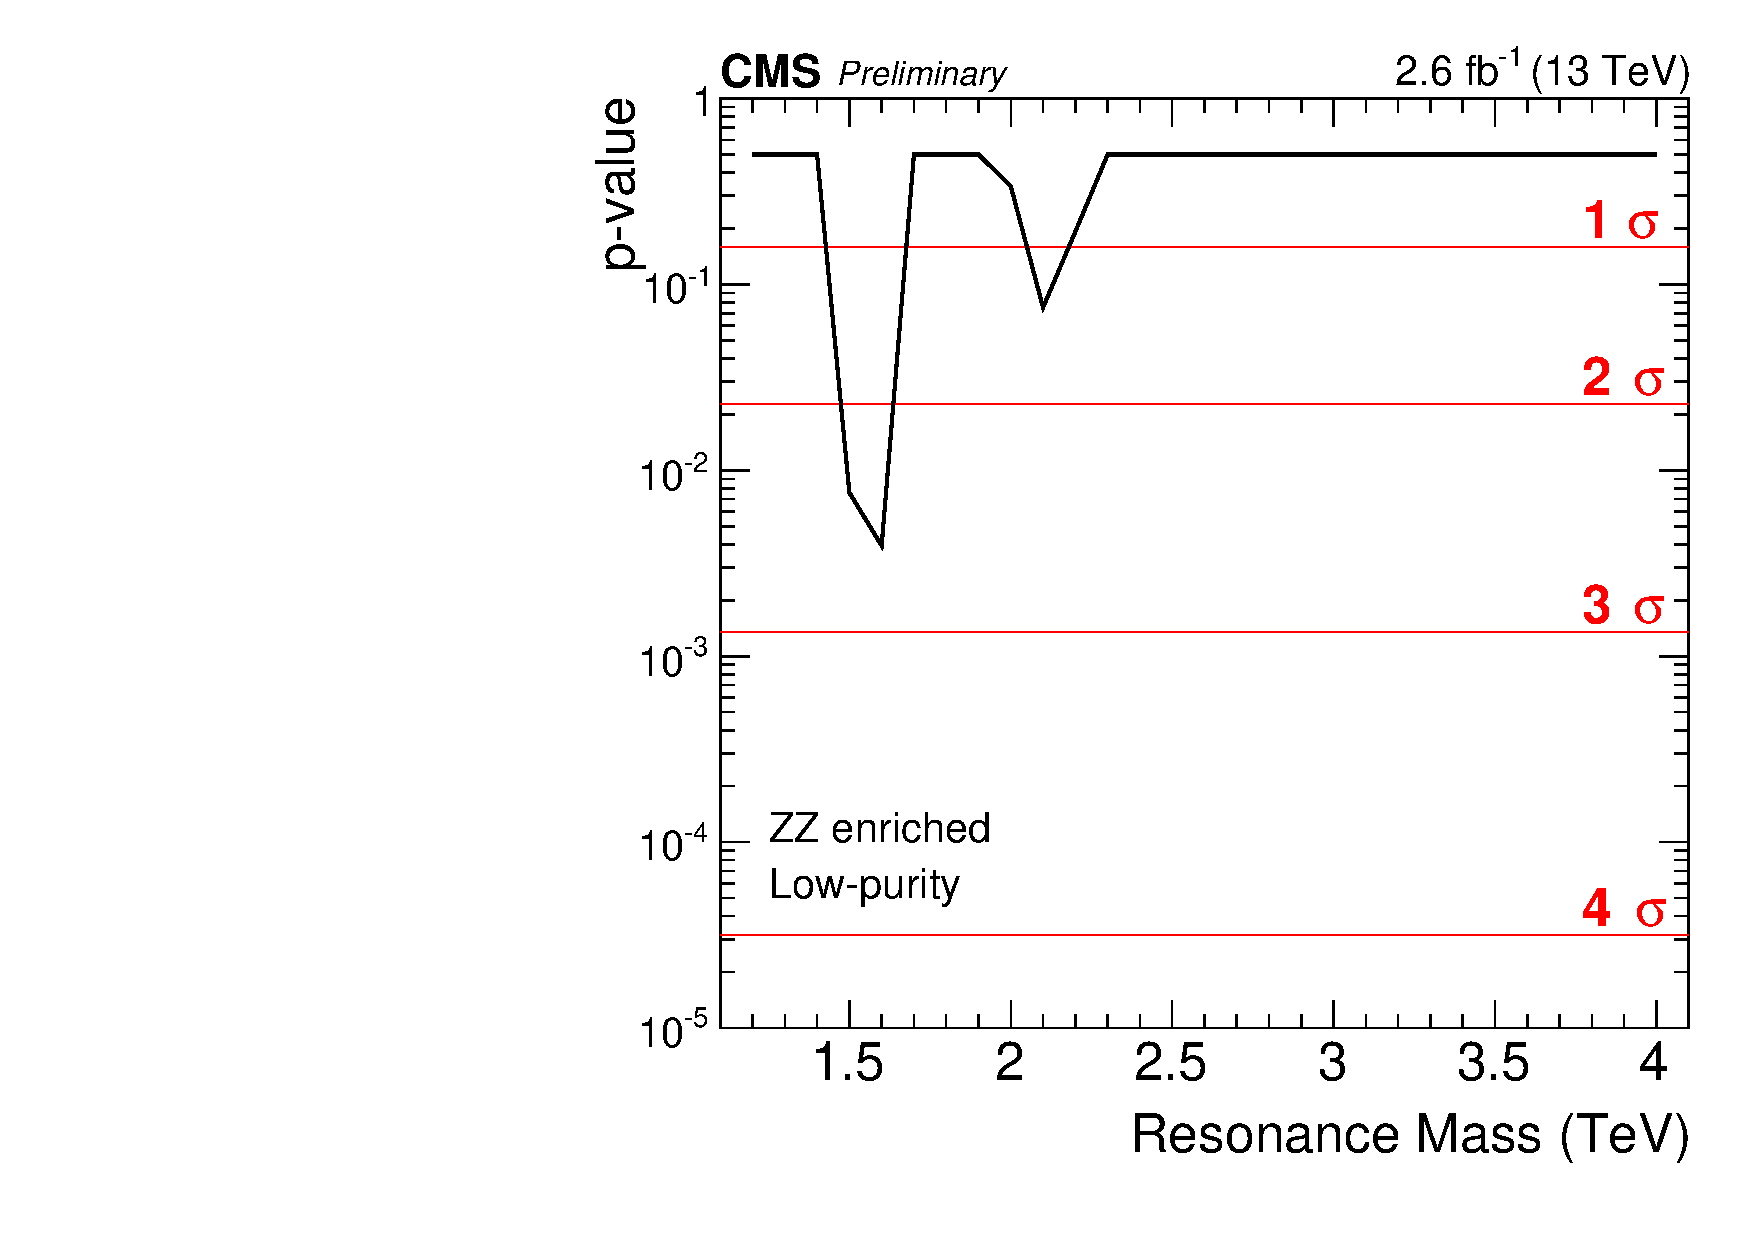
\includegraphics[width=0.327\textwidth]{figures/analysis/search1/AN-15-211/pvalues/pvalue_BulkWWinZZ_low_purity.pdf}
\caption{Expected and observed limits at 95\% CL and corresponding p-values obtained in the different mass categories using 2.6 $\textrm{fb}^{-1}$ of CMS data. Here for a Bulk $G\rightarrow WW$ signal in the LP category.}
\label{fig:app:Limits_LPBulkWW}
\end{figure}
\begin{figure}[h!]
\centering
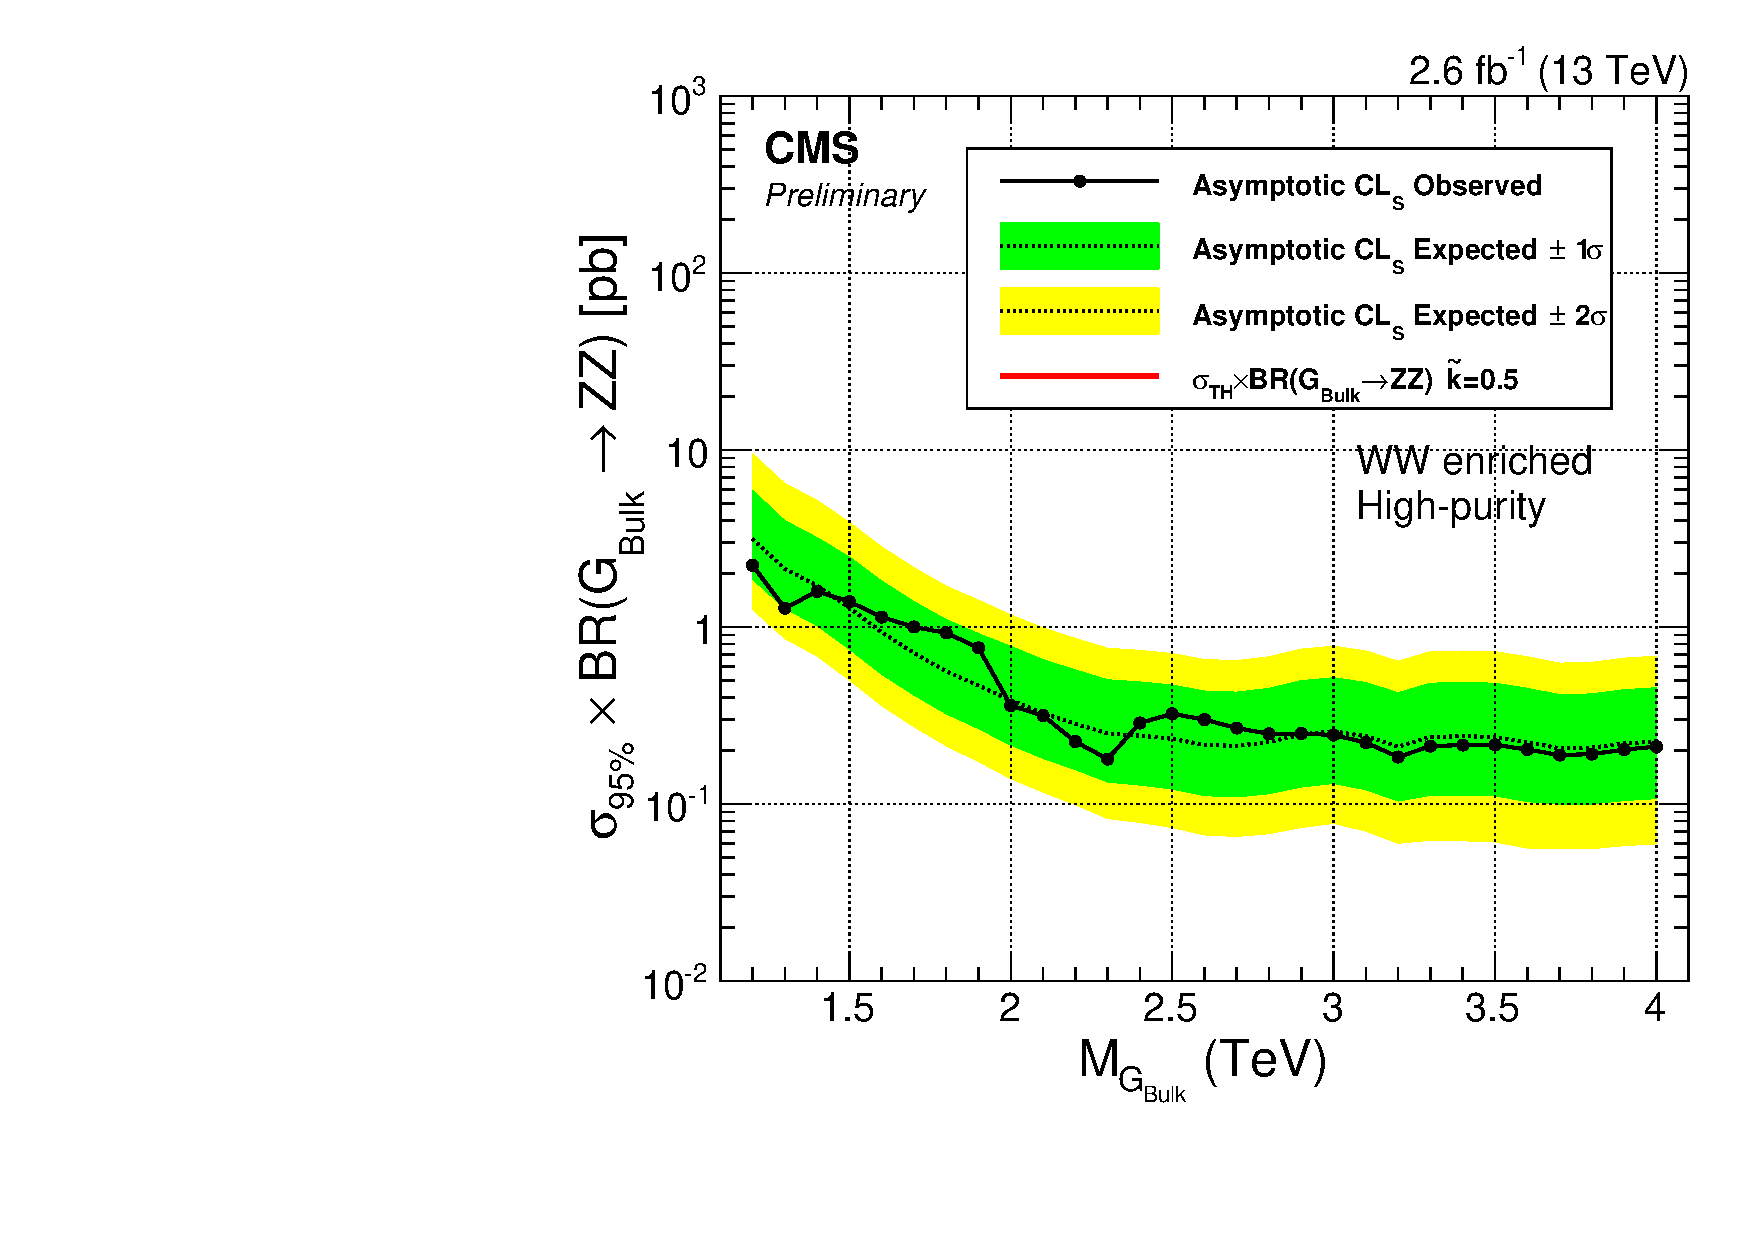
\includegraphics[width=0.327\textwidth]{figures/analysis/search1/AN-15-211/limits/brazilianFlag_BulkZZ_WWHP_13TeV_wPDF.pdf}
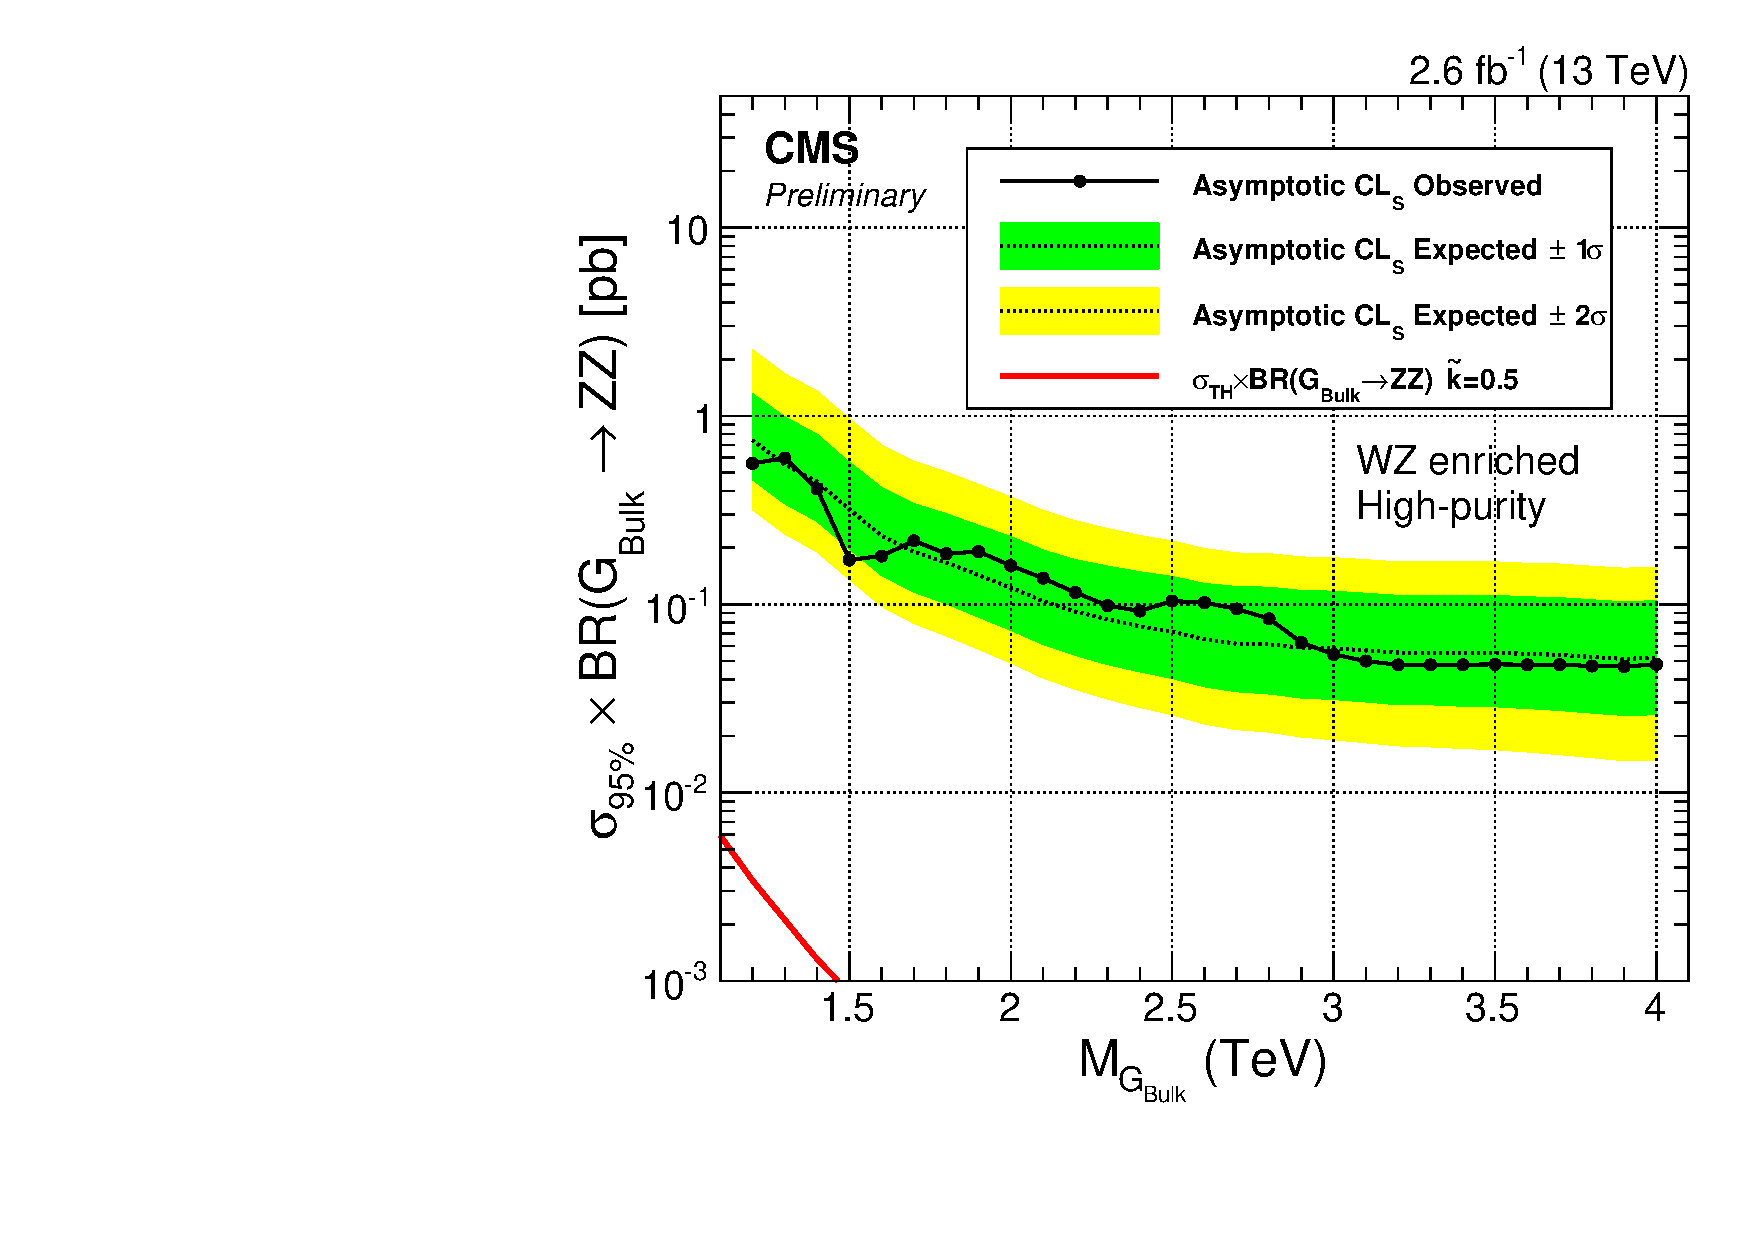
\includegraphics[width=0.327\textwidth]{figures/analysis/search1/AN-15-211/limits/brazilianFlag_BulkZZ_WZHP_13TeV_wPDF.pdf}
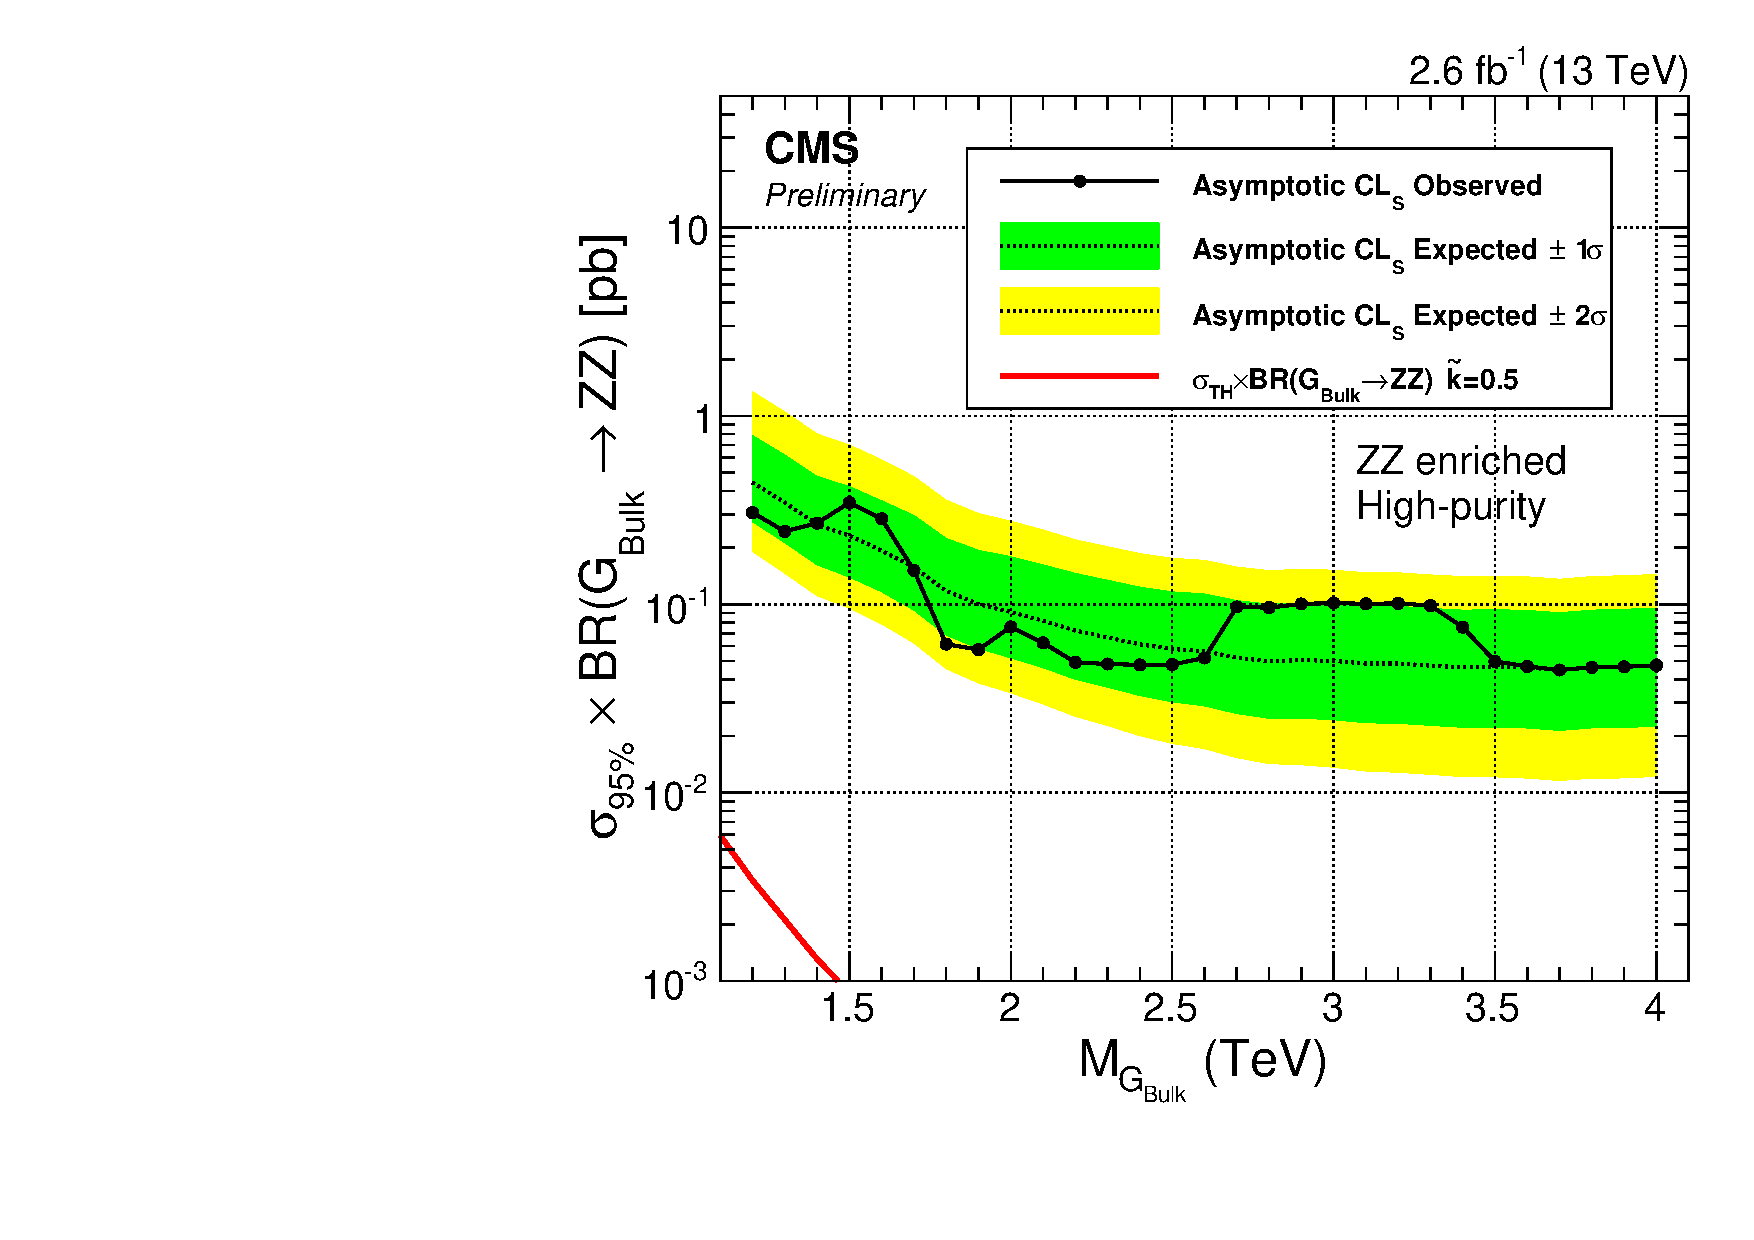
\includegraphics[width=0.327\textwidth]{figures/analysis/search1/AN-15-211/limits/brazilianFlag_BulkZZ_ZZHP_13TeV_wPDF.pdf}\\
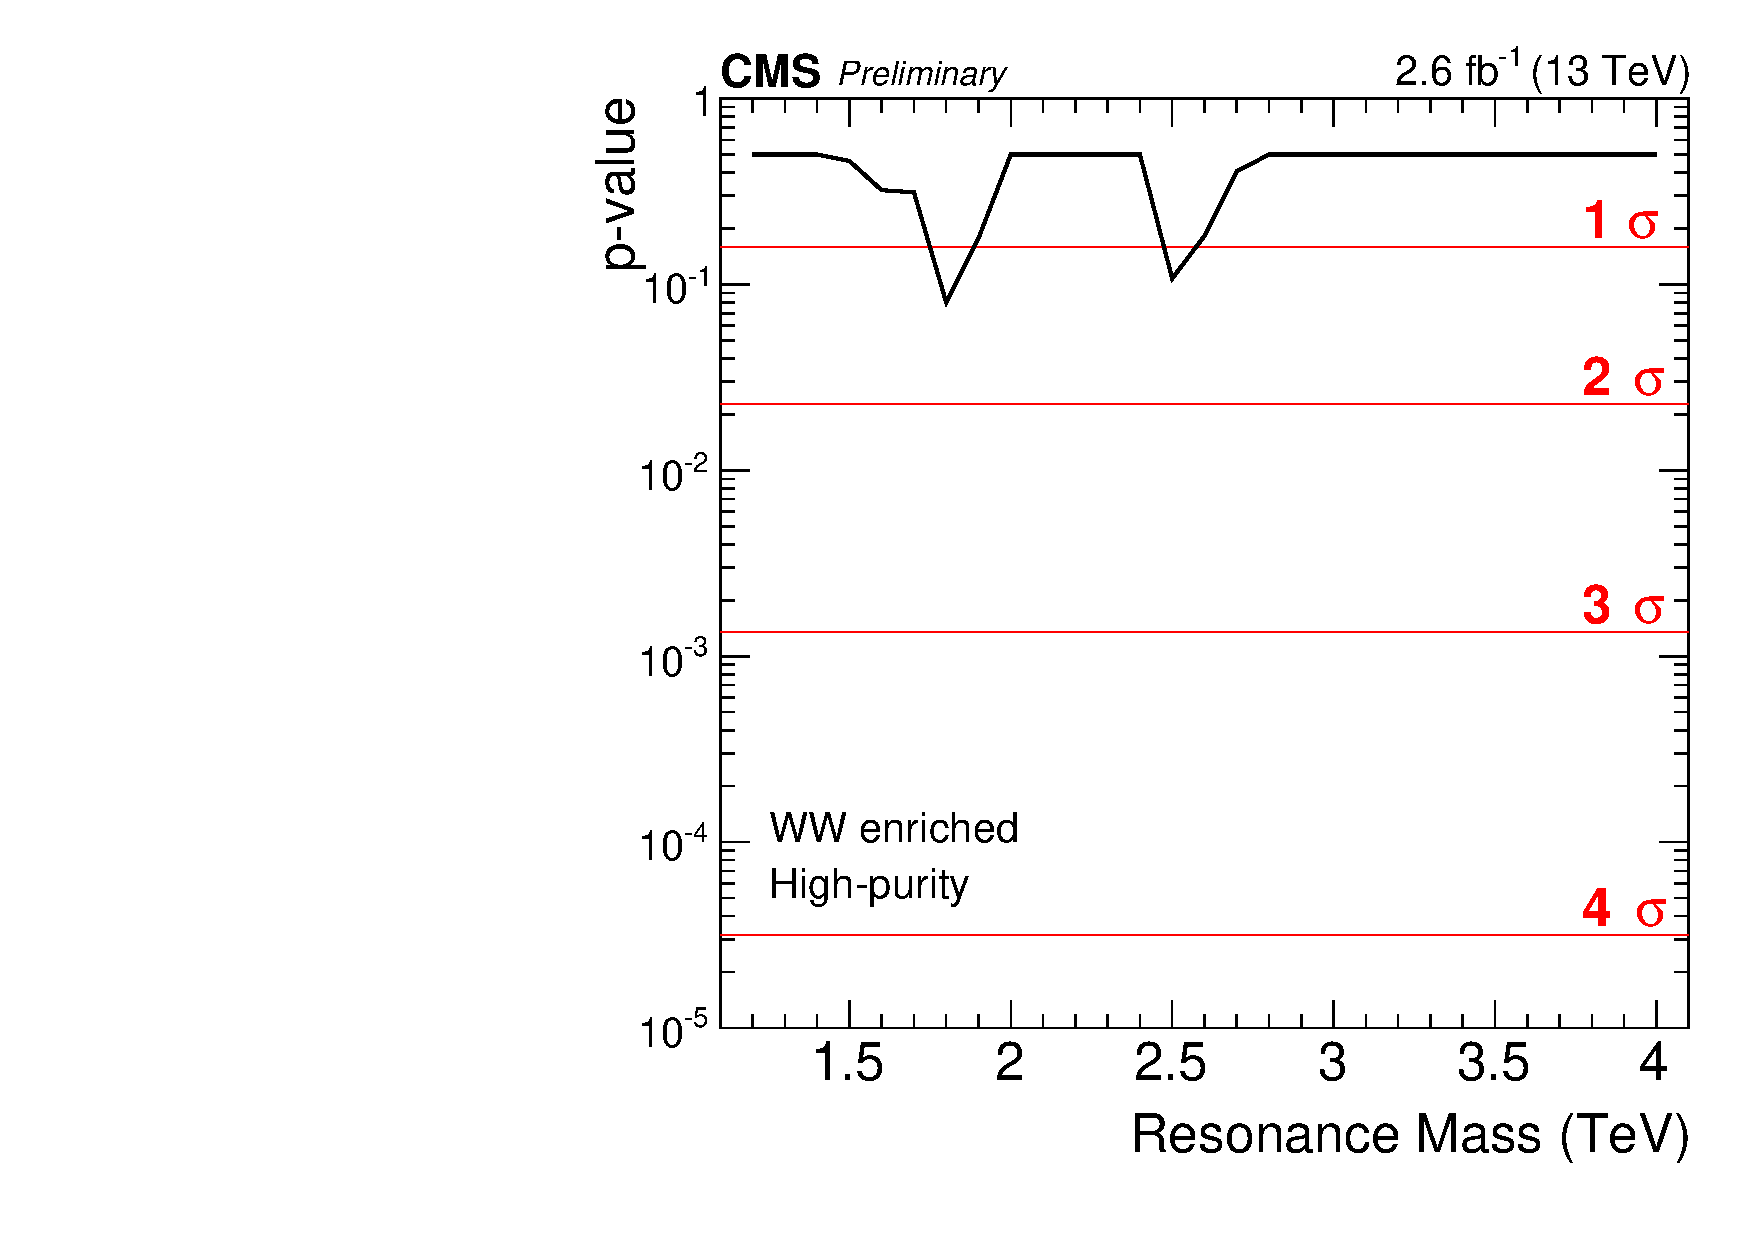
\includegraphics[width=0.327\textwidth]{figures/analysis/search1/AN-15-211/pvalues/pvalue_BulkZZinWW_high_purity.pdf}
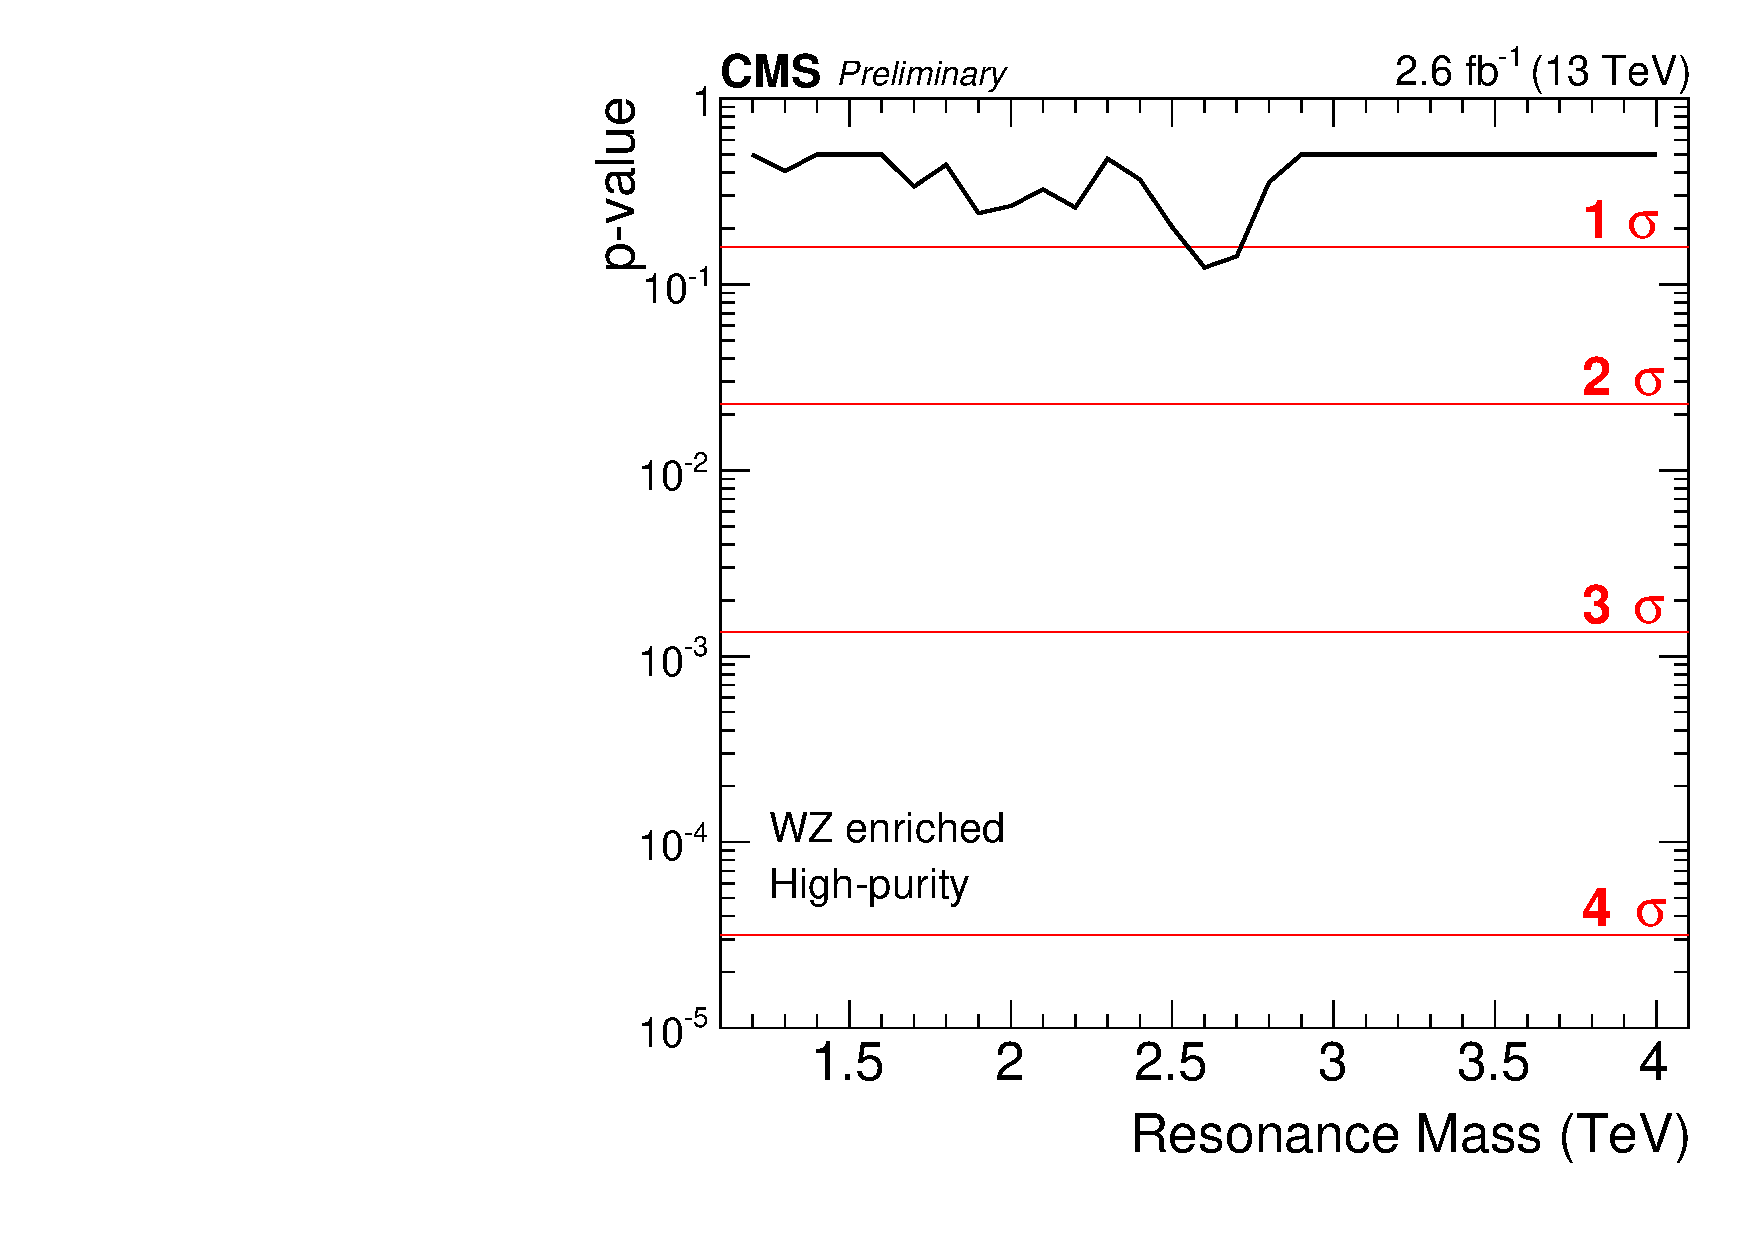
\includegraphics[width=0.327\textwidth]{figures/analysis/search1/AN-15-211/pvalues/pvalue_BulkZZinWZ_high_purity.pdf}
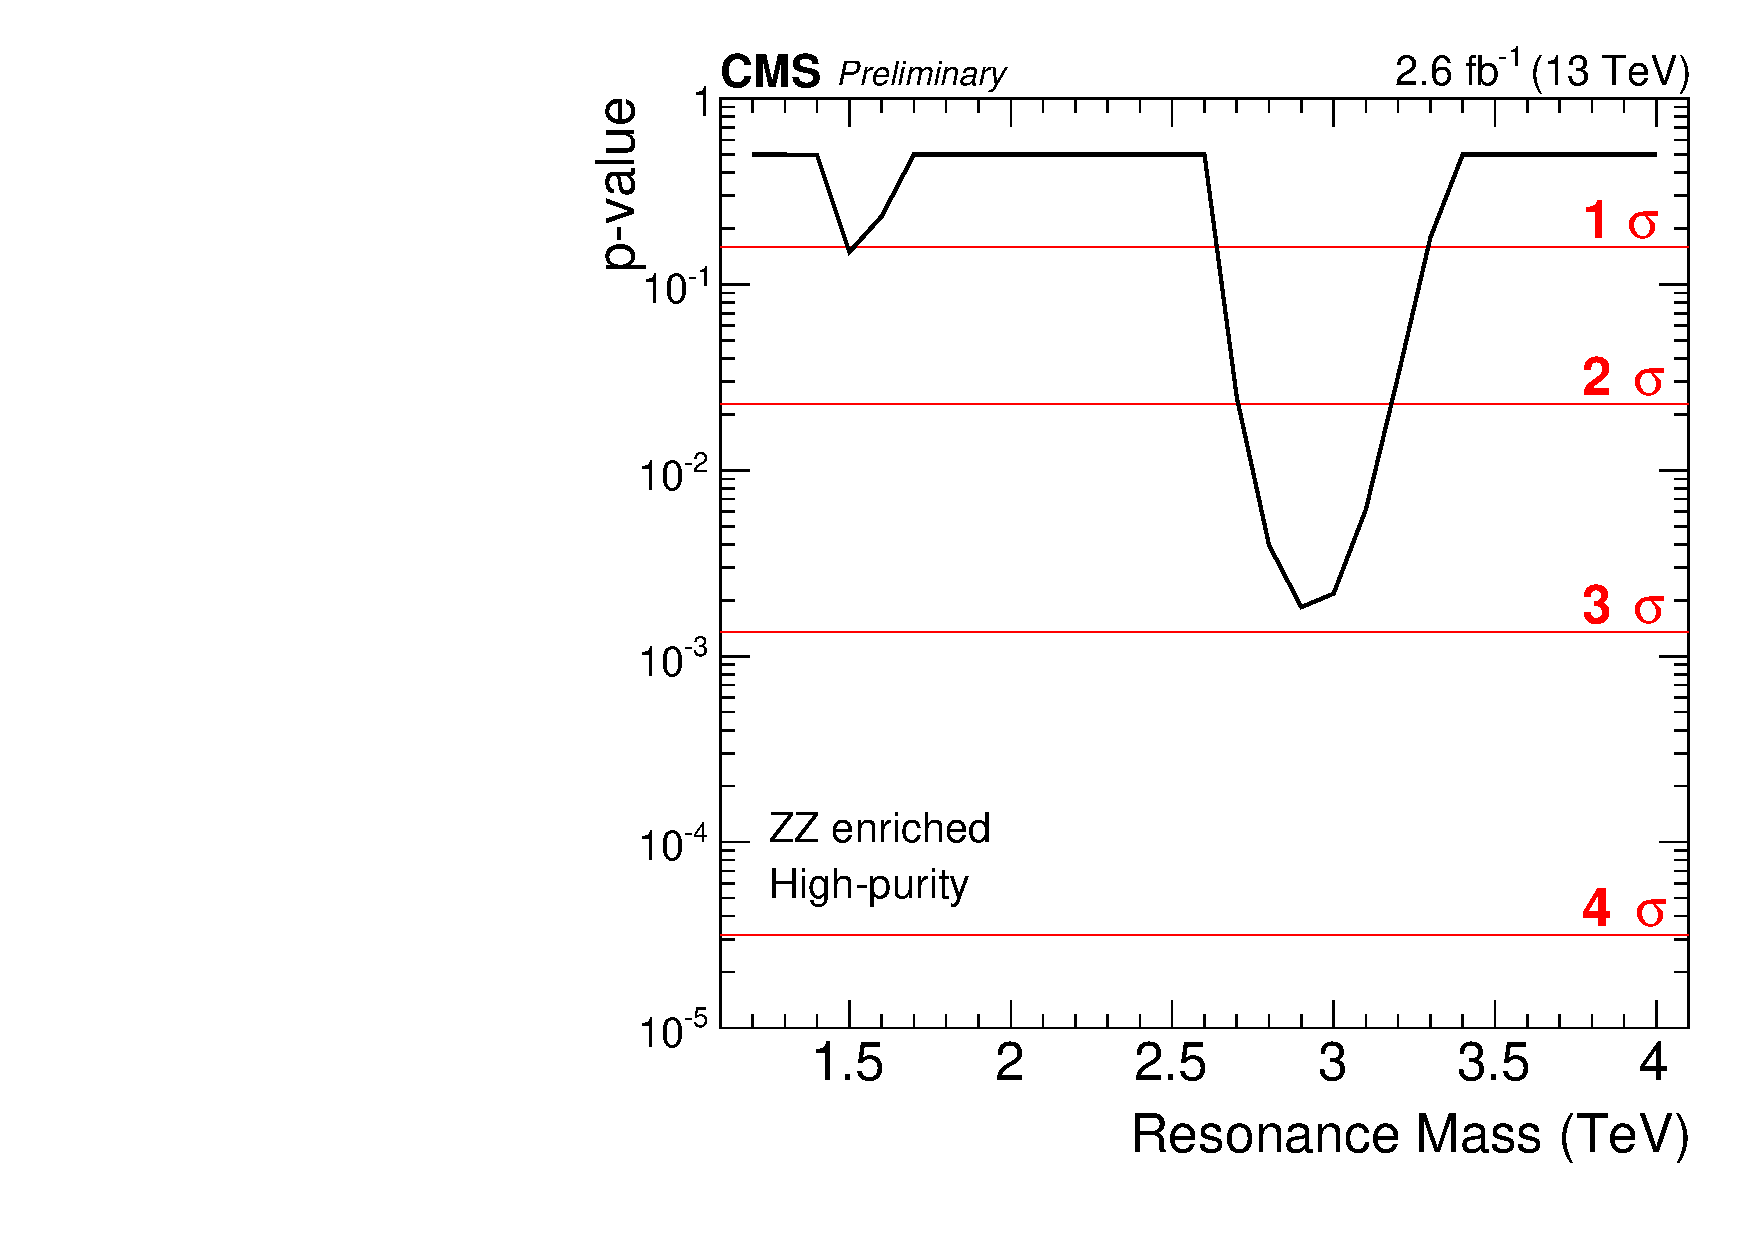
\includegraphics[width=0.327\textwidth]{figures/analysis/search1/AN-15-211/pvalues/pvalue_BulkZZinZZ_high_purity.pdf}
\caption{Expected and observed limits at 95\% CL and corresponding p-values obtained in the different mass categories. Here for a $G\rightarrow ZZ$ signal in the HP category.}
\label{fig:app:Limits_HPBulkZZ}
\end{figure}
\begin{figure}[h!]
\centering
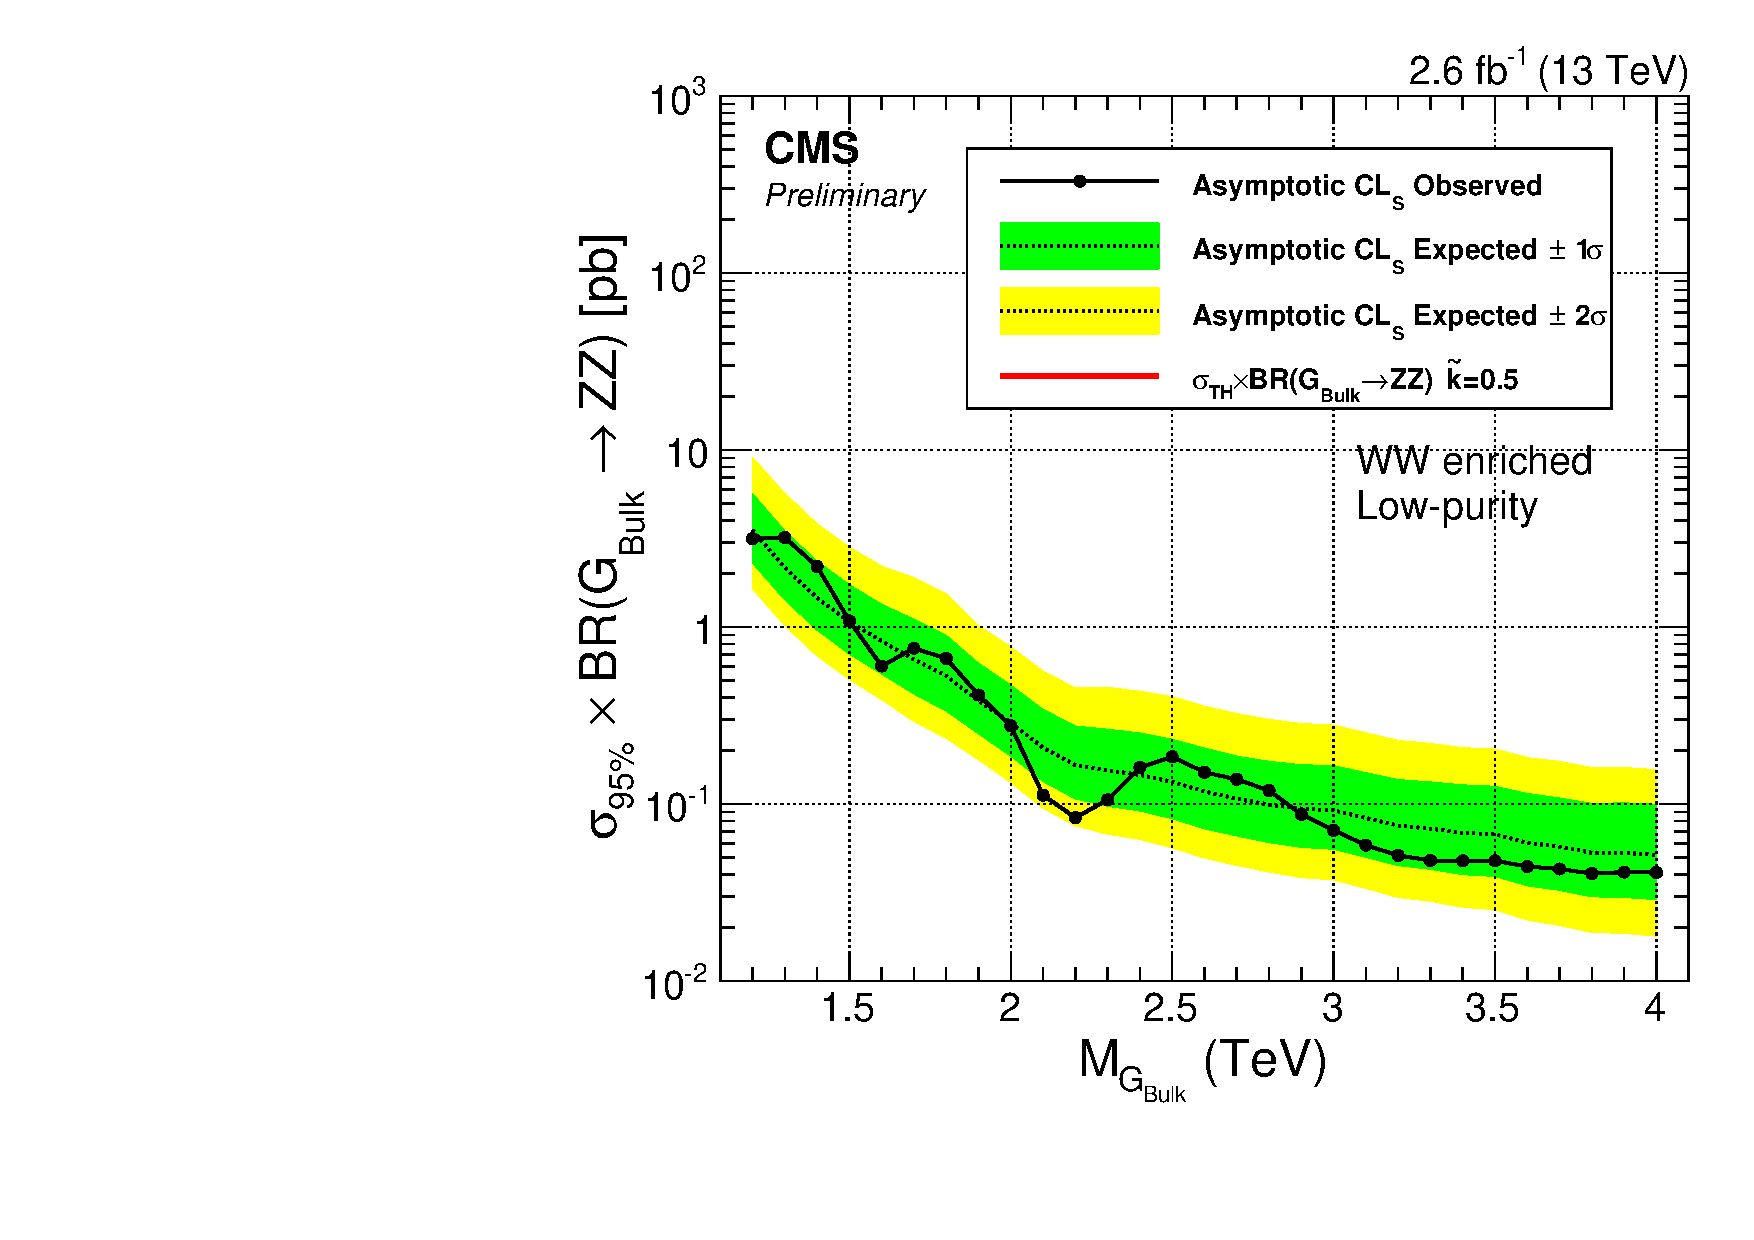
\includegraphics[width=0.327\textwidth]{figures/analysis/search1/AN-15-211/limits/brazilianFlag_BulkZZ_WWLP_13TeV_wPDF.pdf}
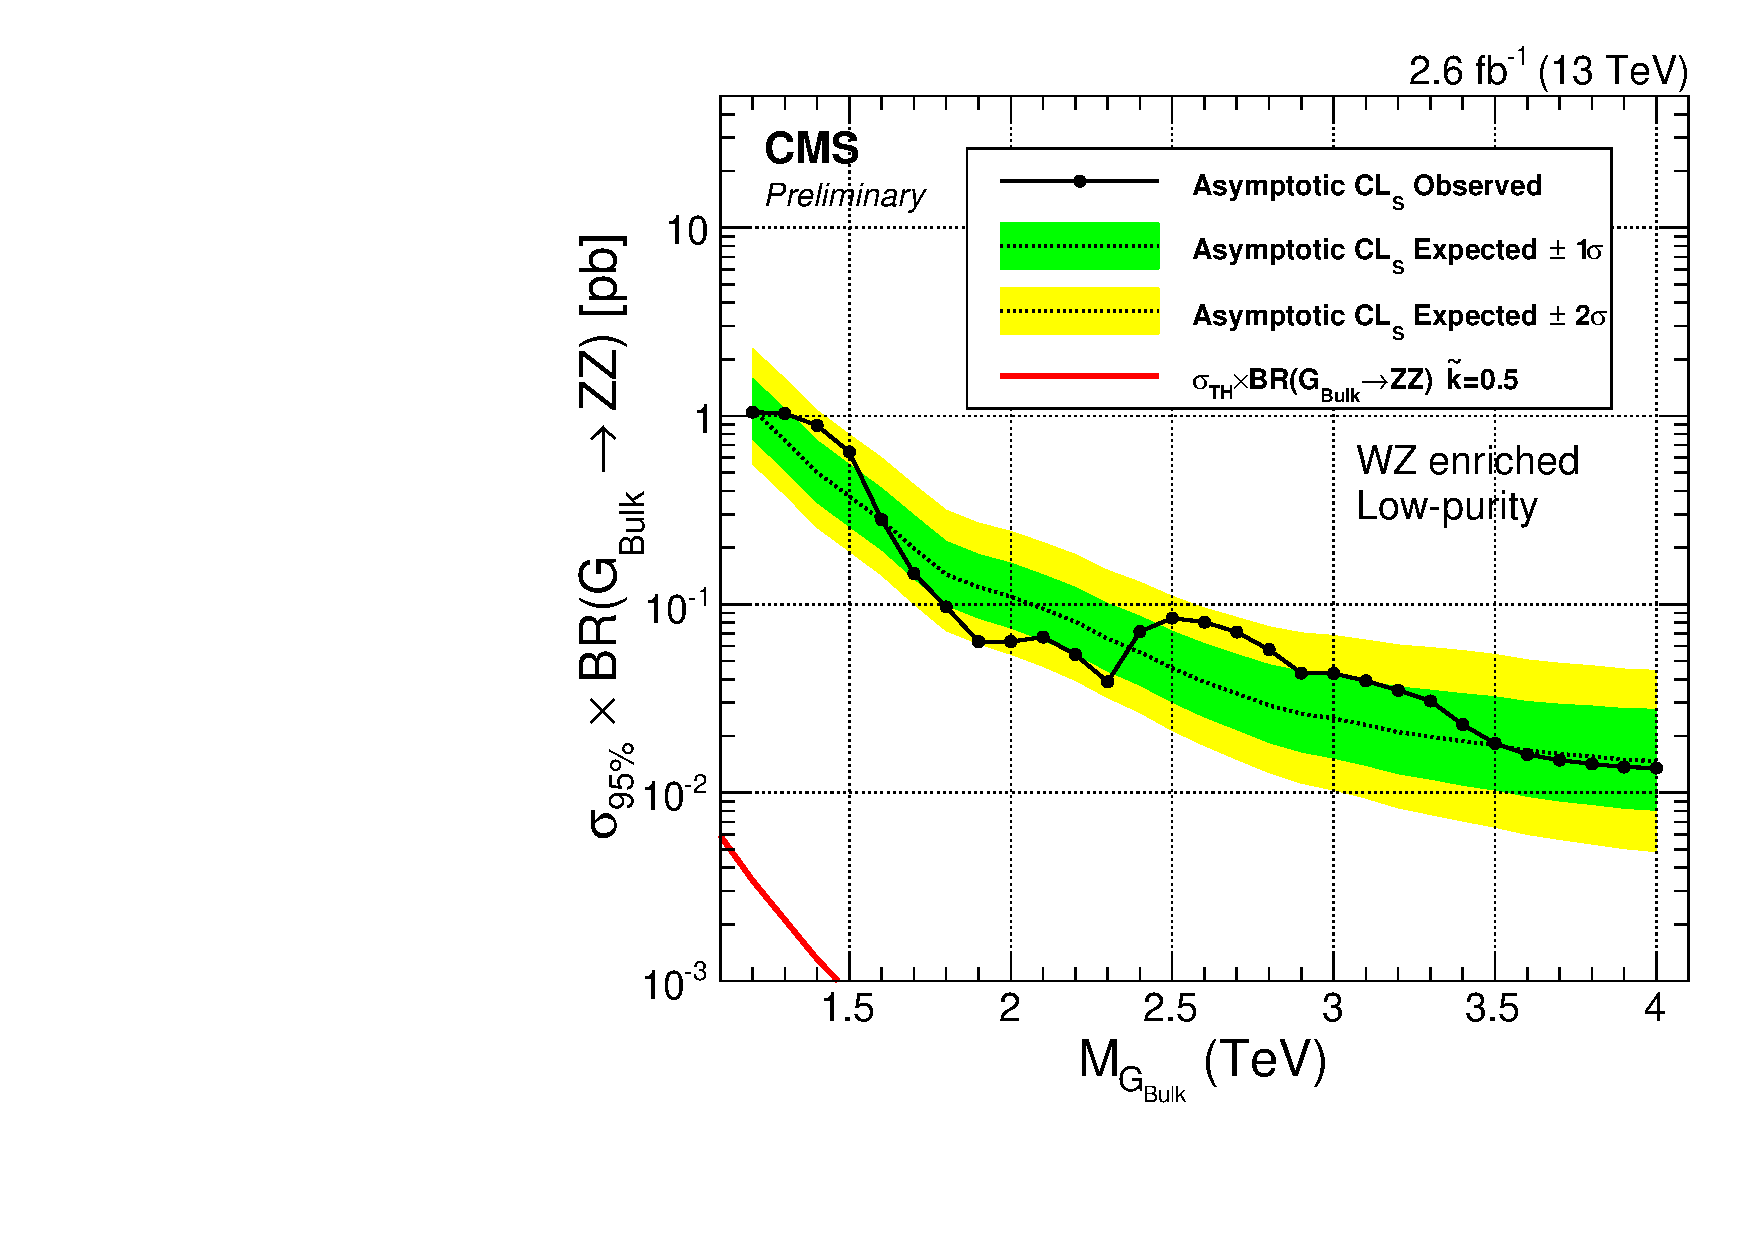
\includegraphics[width=0.327\textwidth]{figures/analysis/search1/AN-15-211/limits/brazilianFlag_BulkZZ_WZLP_13TeV_wPDF.pdf}
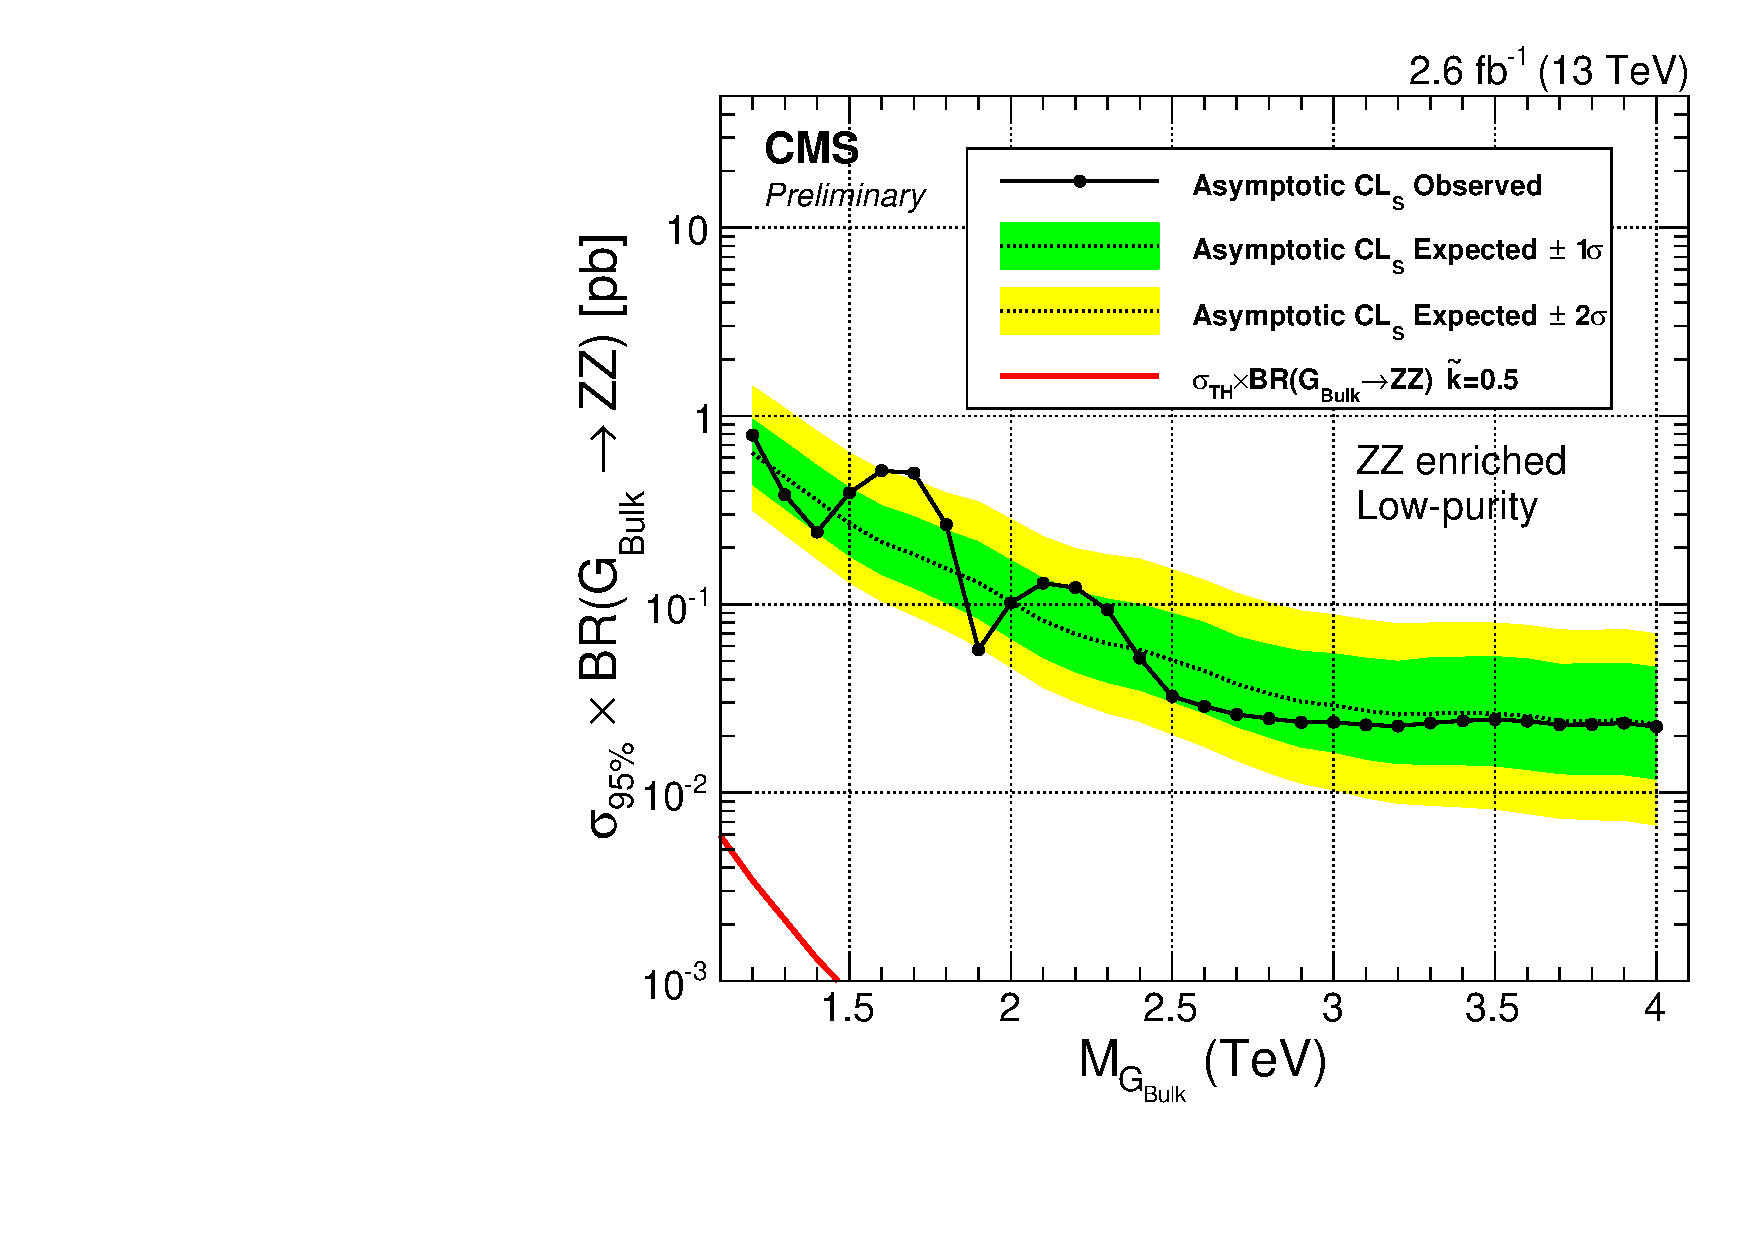
\includegraphics[width=0.327\textwidth]{figures/analysis/search1/AN-15-211/limits/brazilianFlag_BulkZZ_ZZLP_13TeV_wPDF.pdf}\\
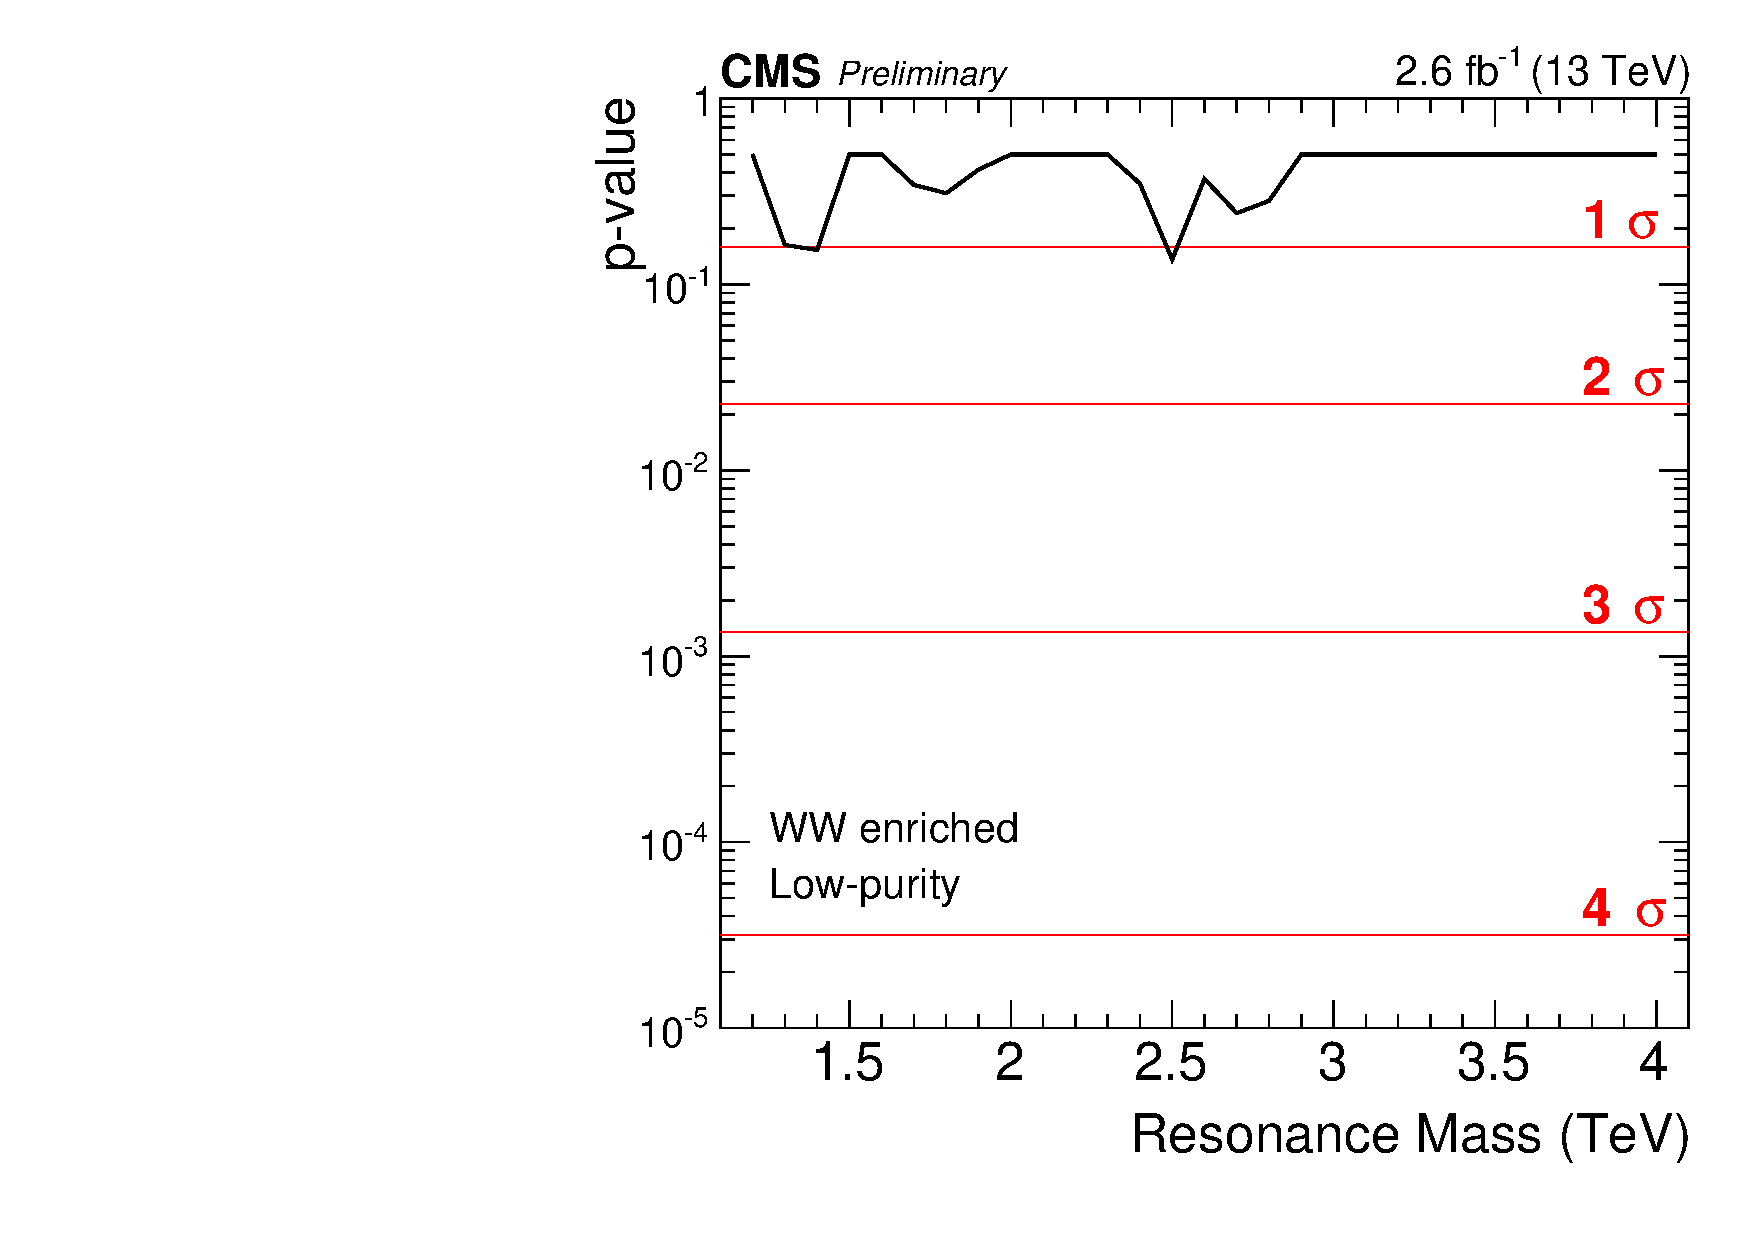
\includegraphics[width=0.327\textwidth]{figures/analysis/search1/AN-15-211/pvalues/pvalue_BulkZZinWW_low_purity.pdf}
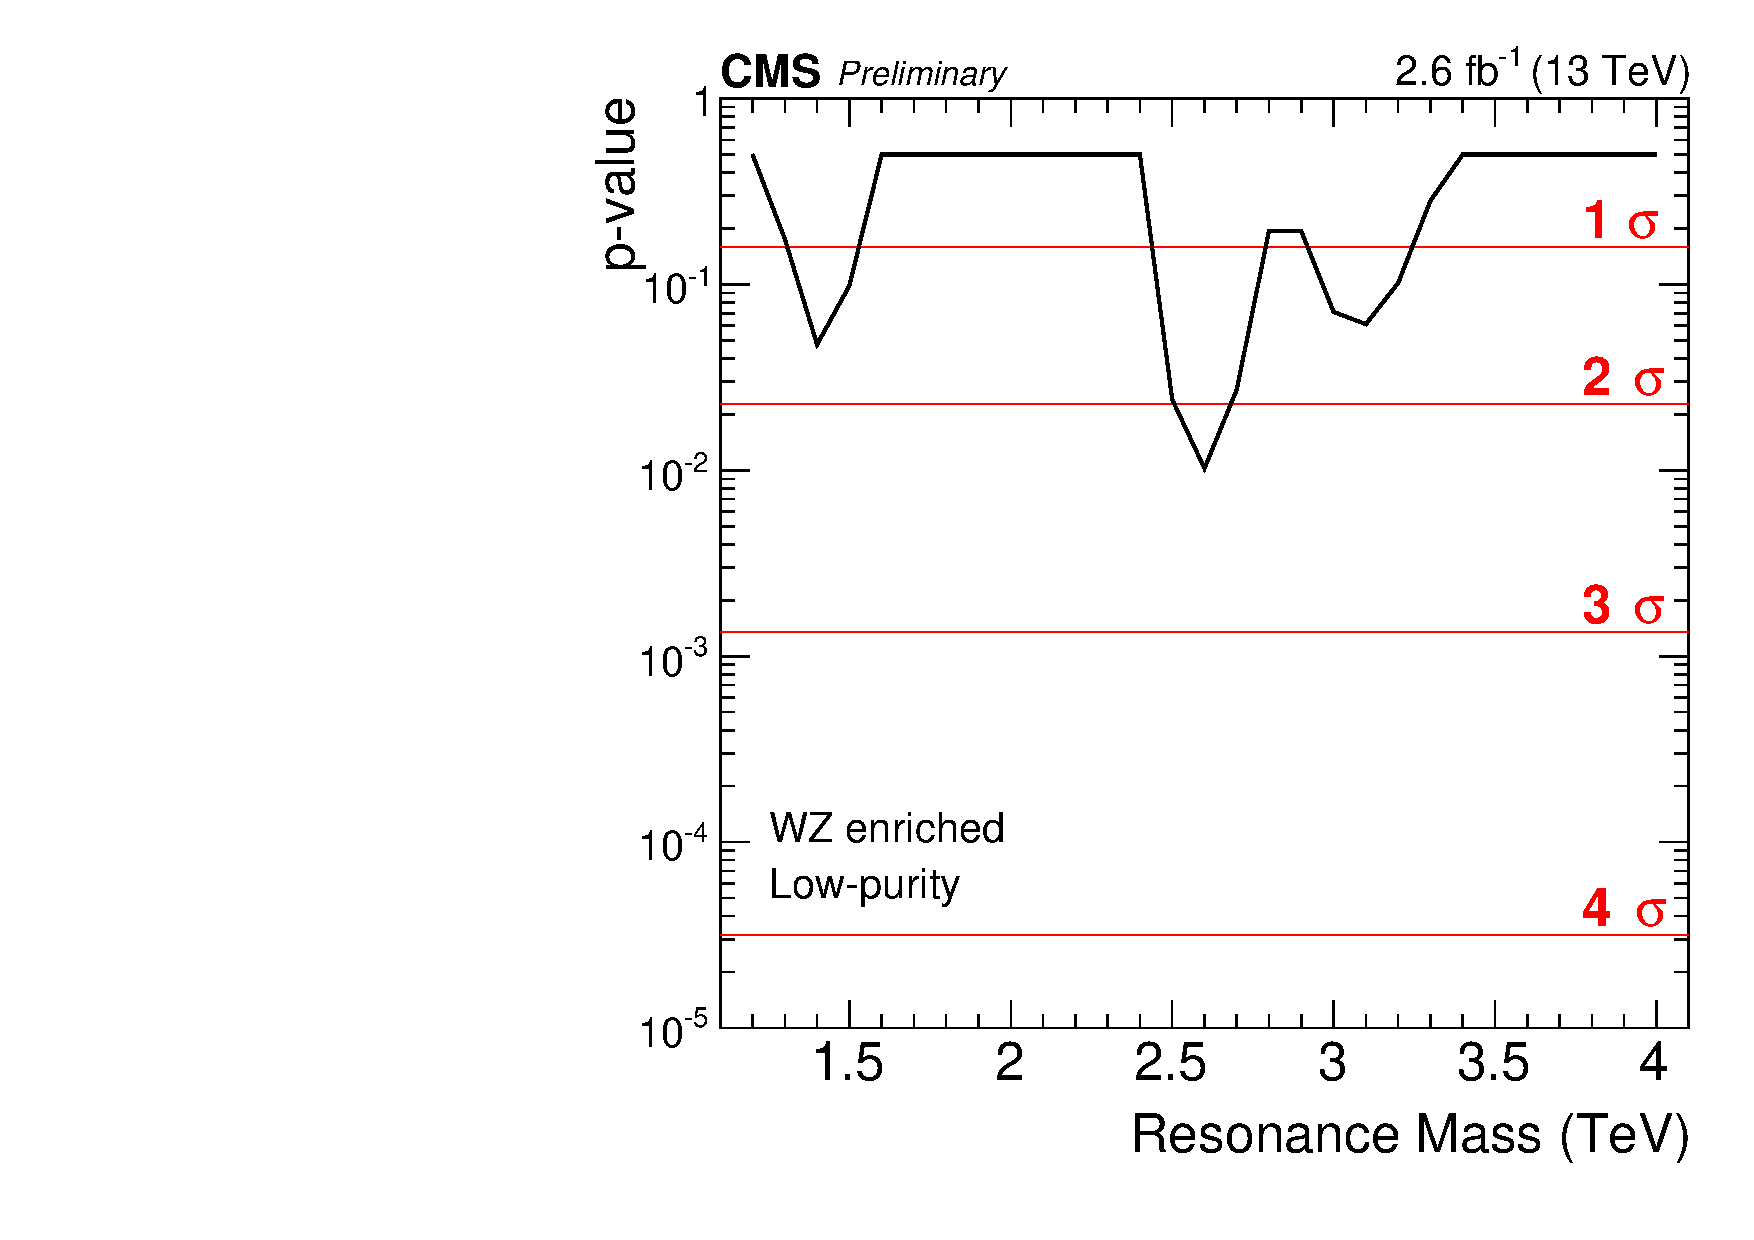
\includegraphics[width=0.327\textwidth]{figures/analysis/search1/AN-15-211/pvalues/pvalue_BulkZZinWZ_low_purity.pdf}
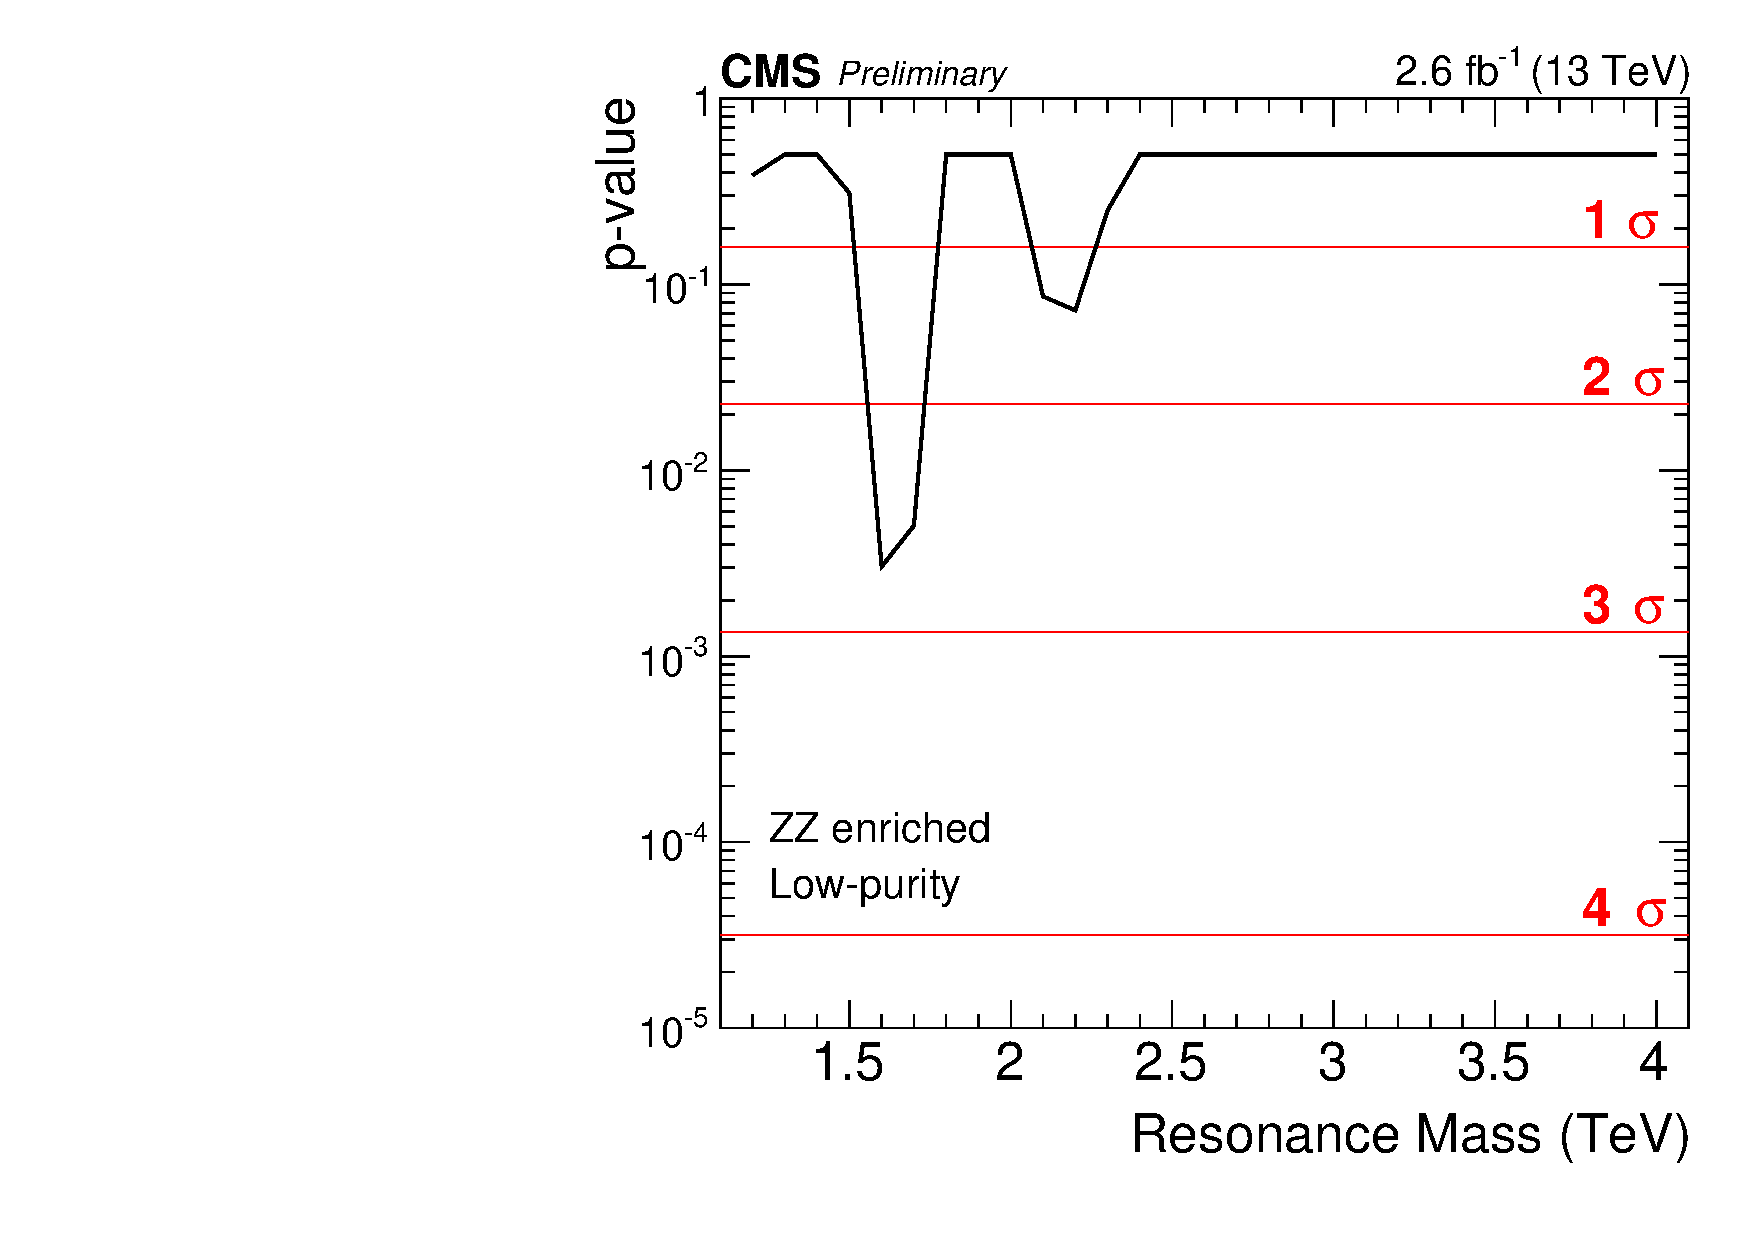
\includegraphics[width=0.327\textwidth]{figures/analysis/search1/AN-15-211/pvalues/pvalue_BulkZZinZZ_low_purity.pdf}
\caption{Expected and observed limits at 95\% CL and corresponding p-values obtained in the different mass categories. Here for a $G\rightarrow ZZ$ signal in the LP category.}
\label{fig:app:Limits_LPBulkZZ}
\end{figure}
\begin{figure}[h!]
\centering
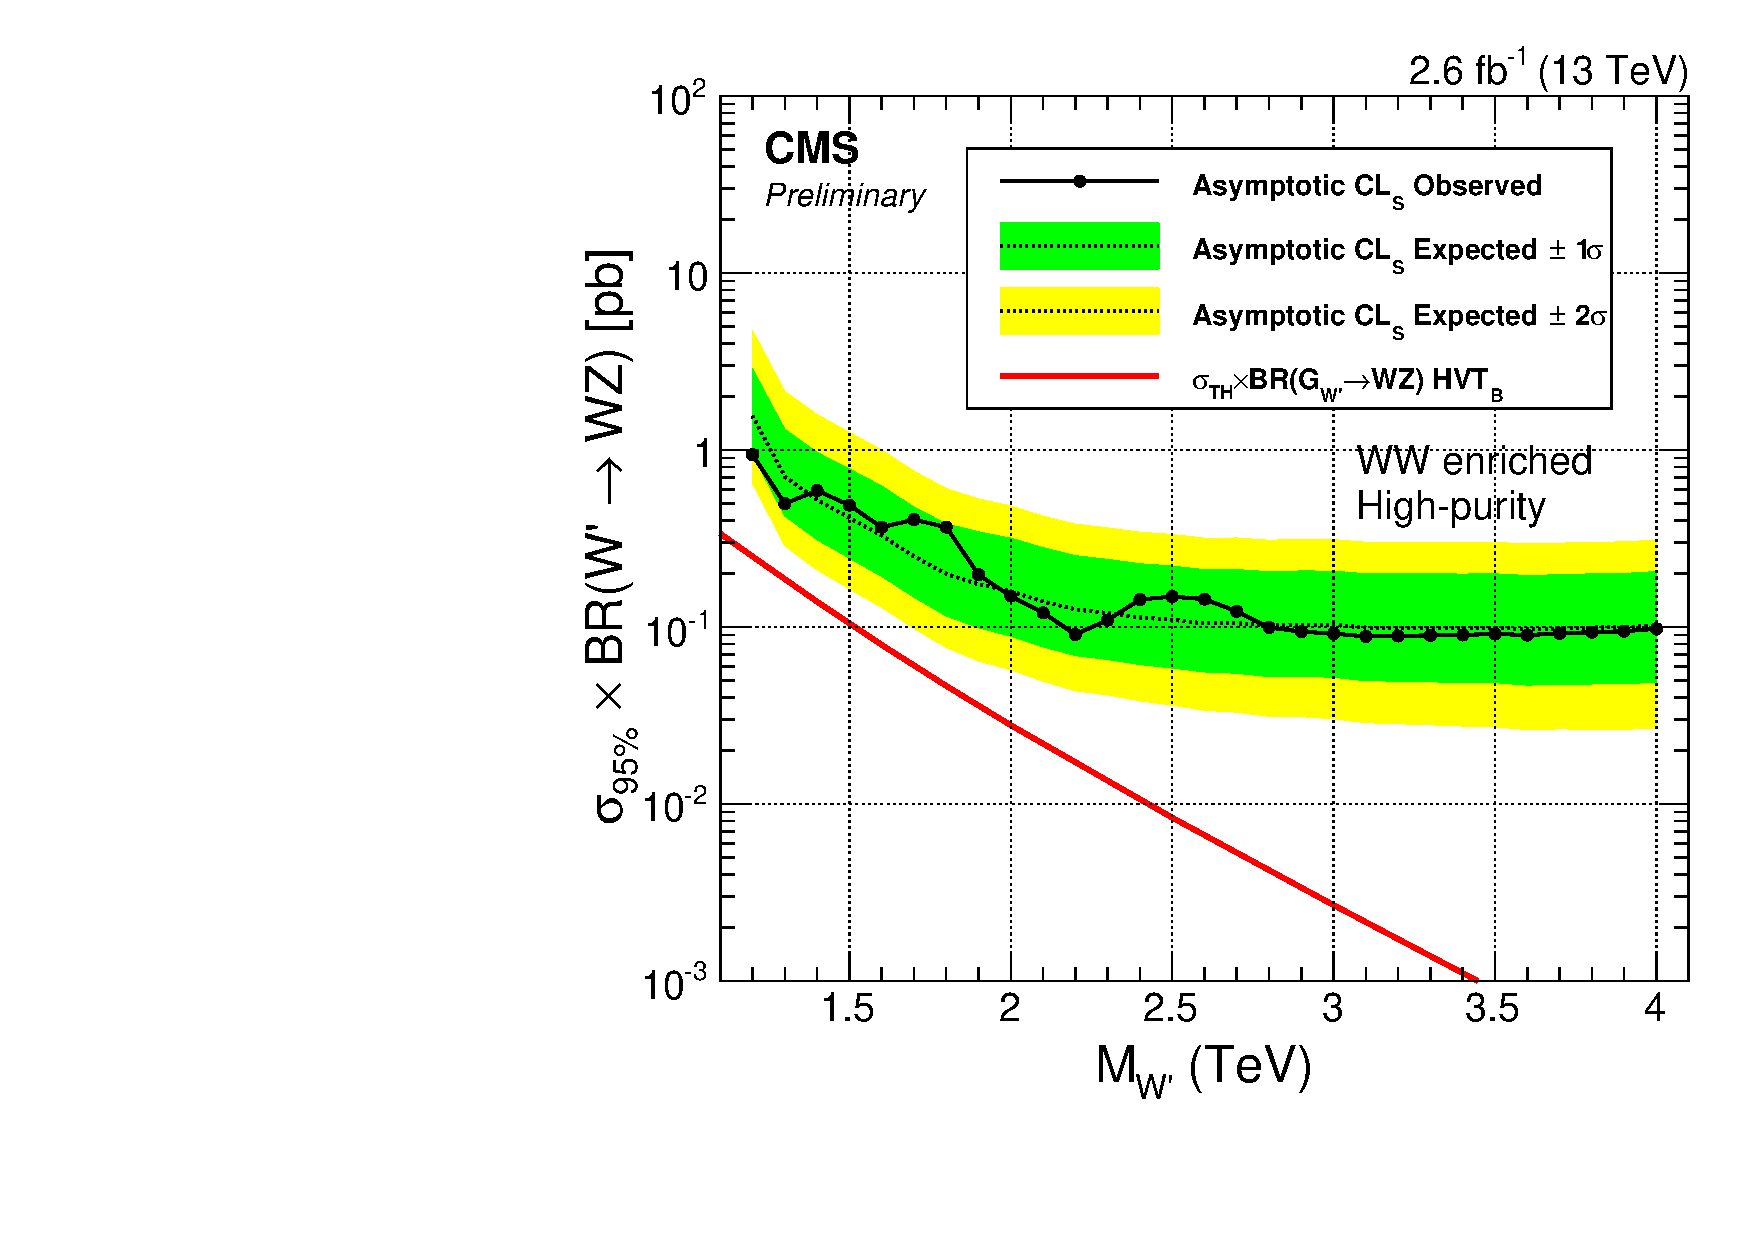
\includegraphics[width=0.327\textwidth]{figures/analysis/search1/AN-15-211/limits/brazilianFlag_WZ_WWHP_13TeV_wPDF.pdf}
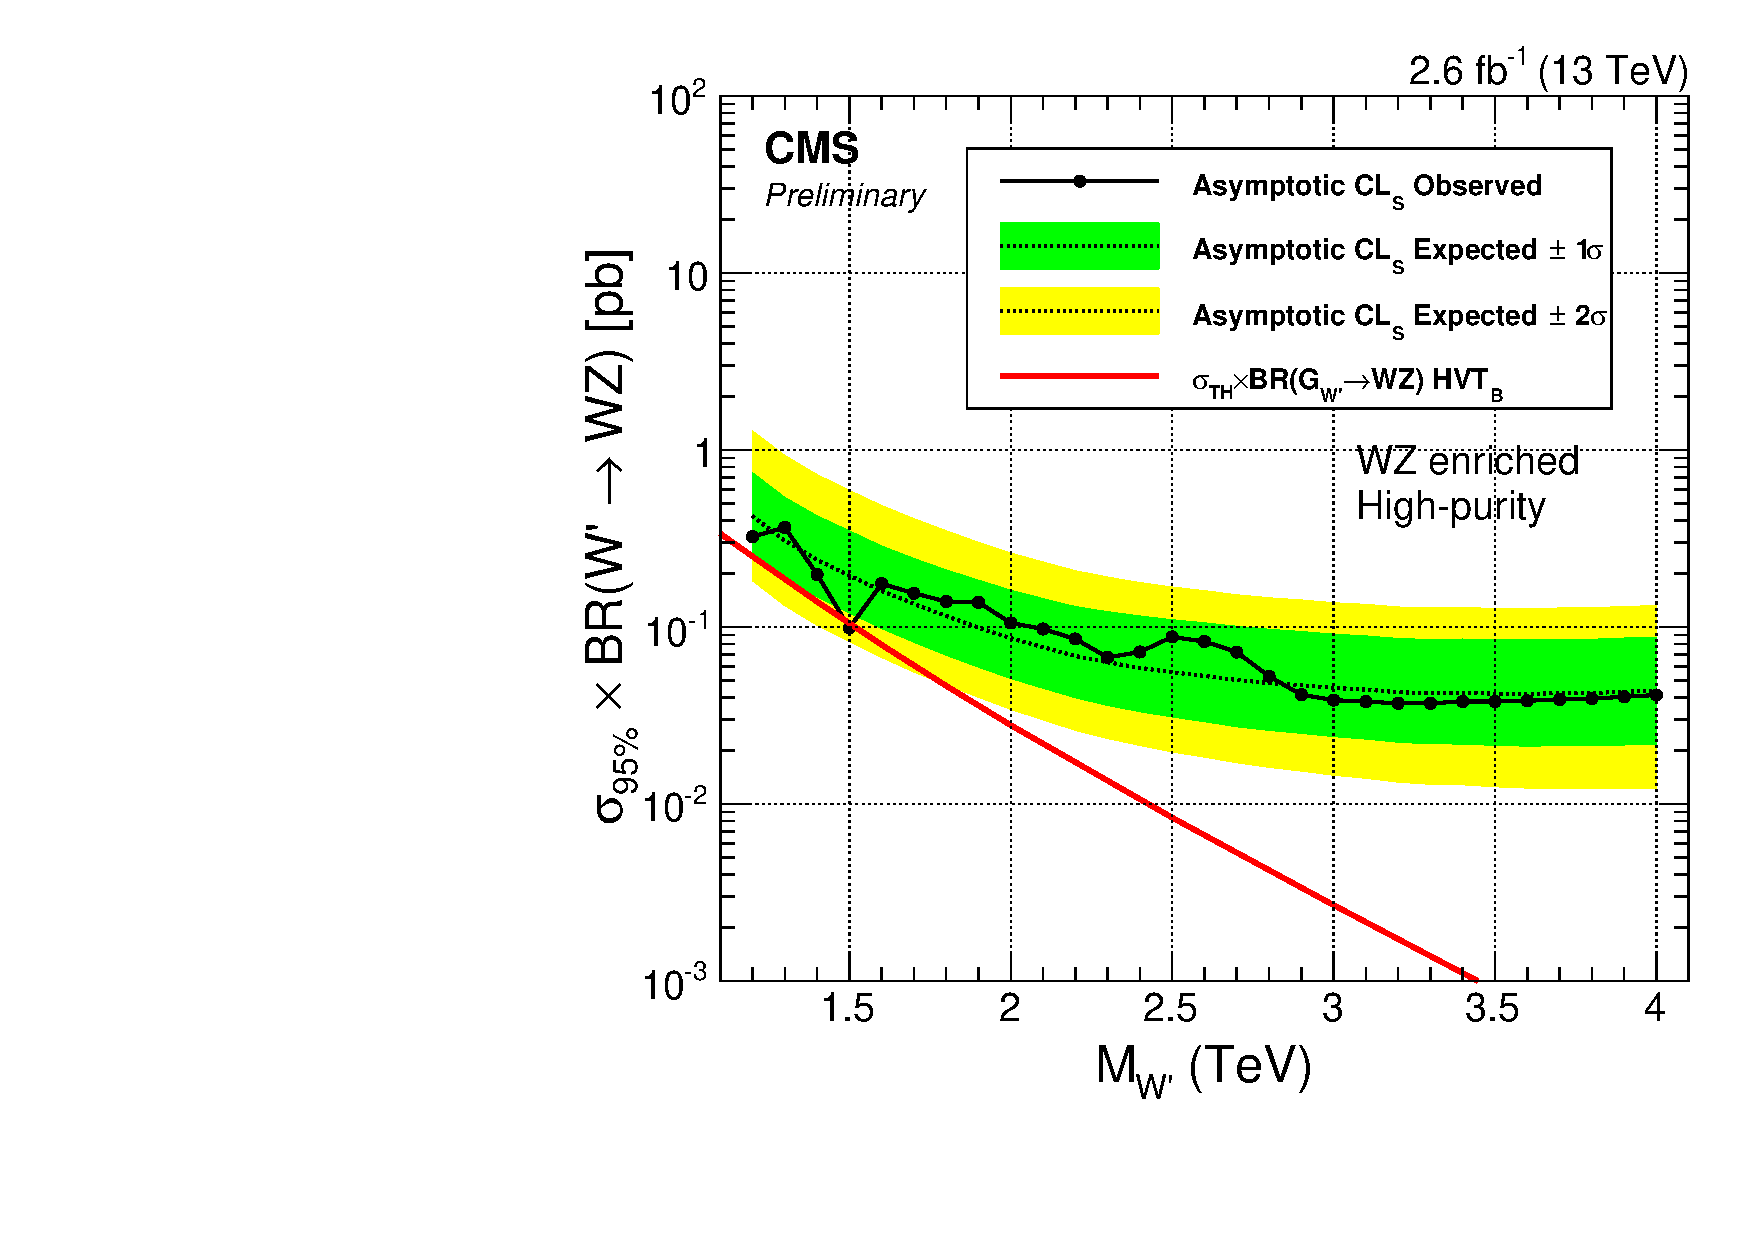
\includegraphics[width=0.327\textwidth]{figures/analysis/search1/AN-15-211/limits/brazilianFlag_WZ_WZHP_13TeV_wPDF.pdf}
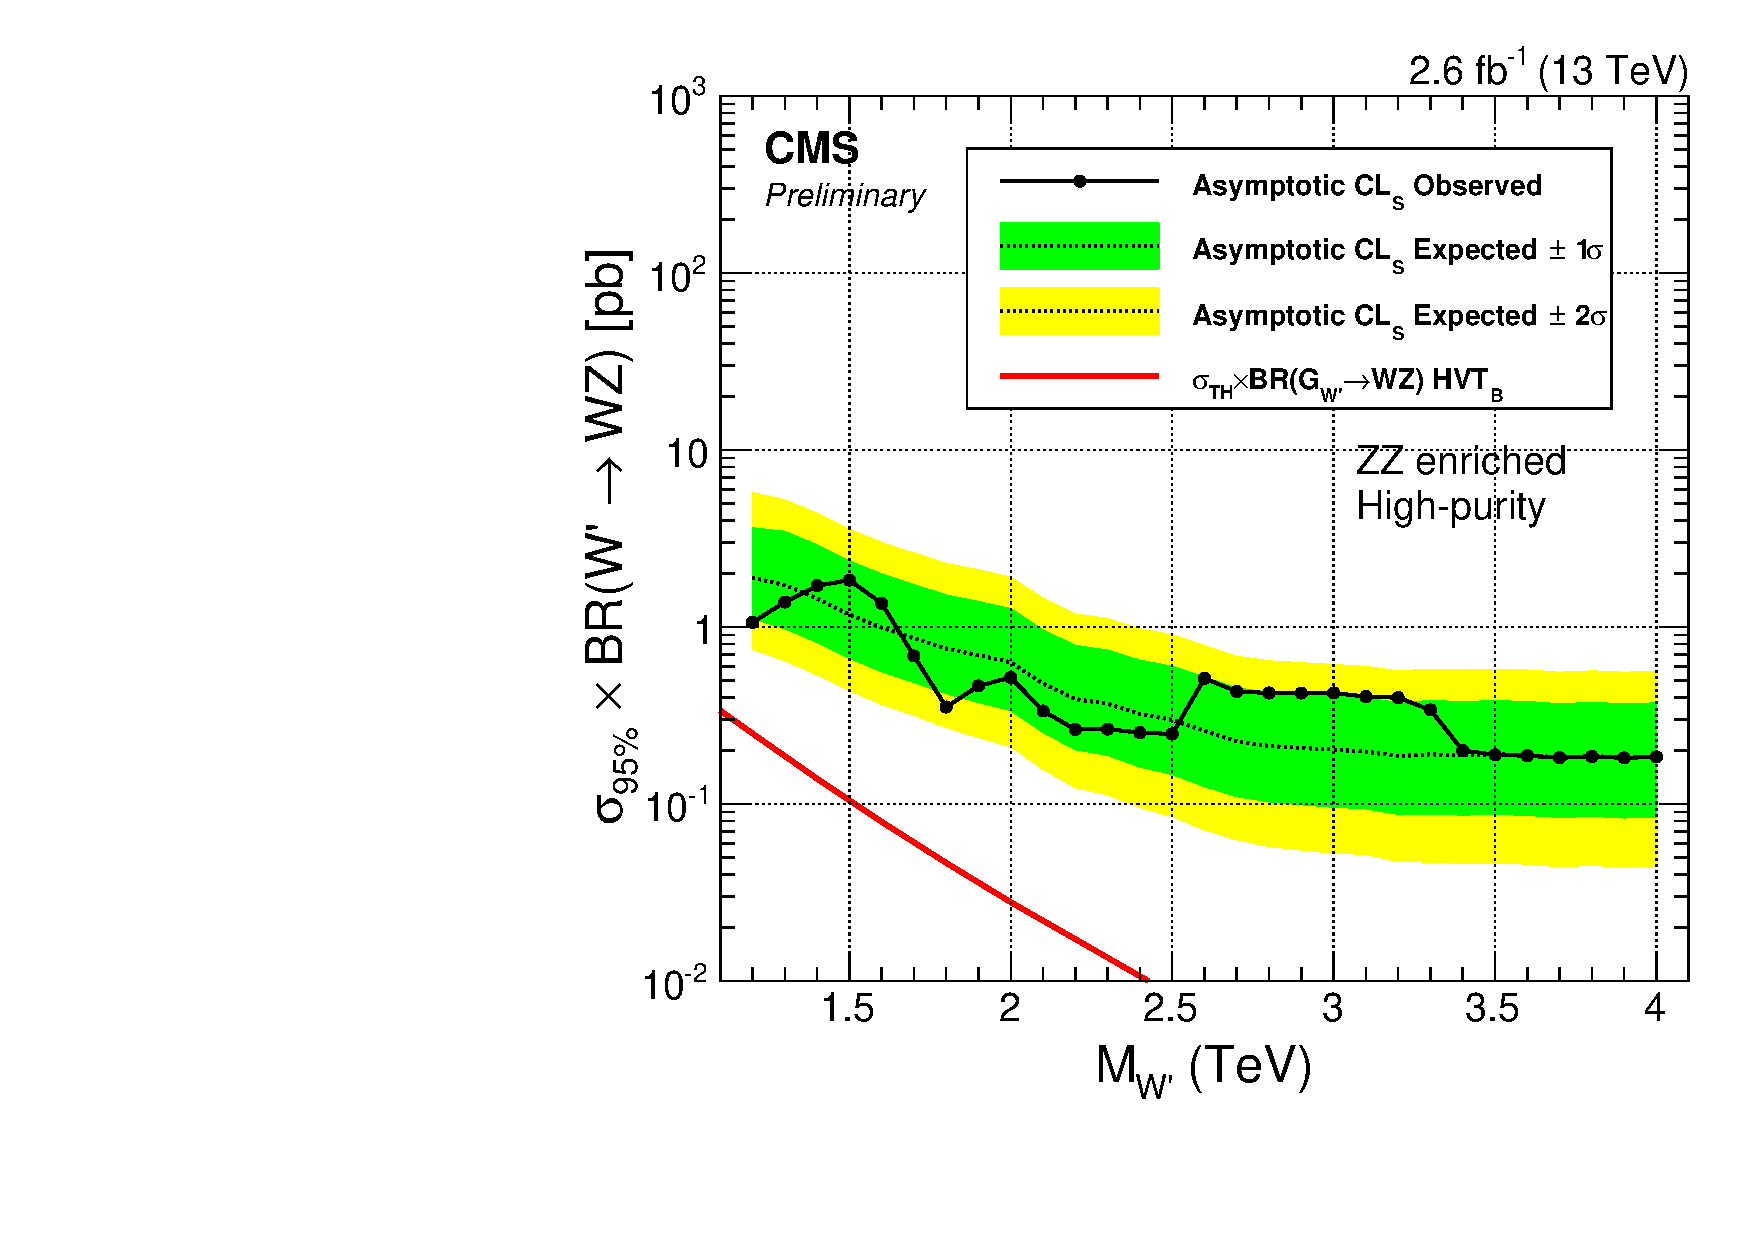
\includegraphics[width=0.327\textwidth]{figures/analysis/search1/AN-15-211/limits/brazilianFlag_WZ_ZZHP_13TeV_wPDF.pdf}\\
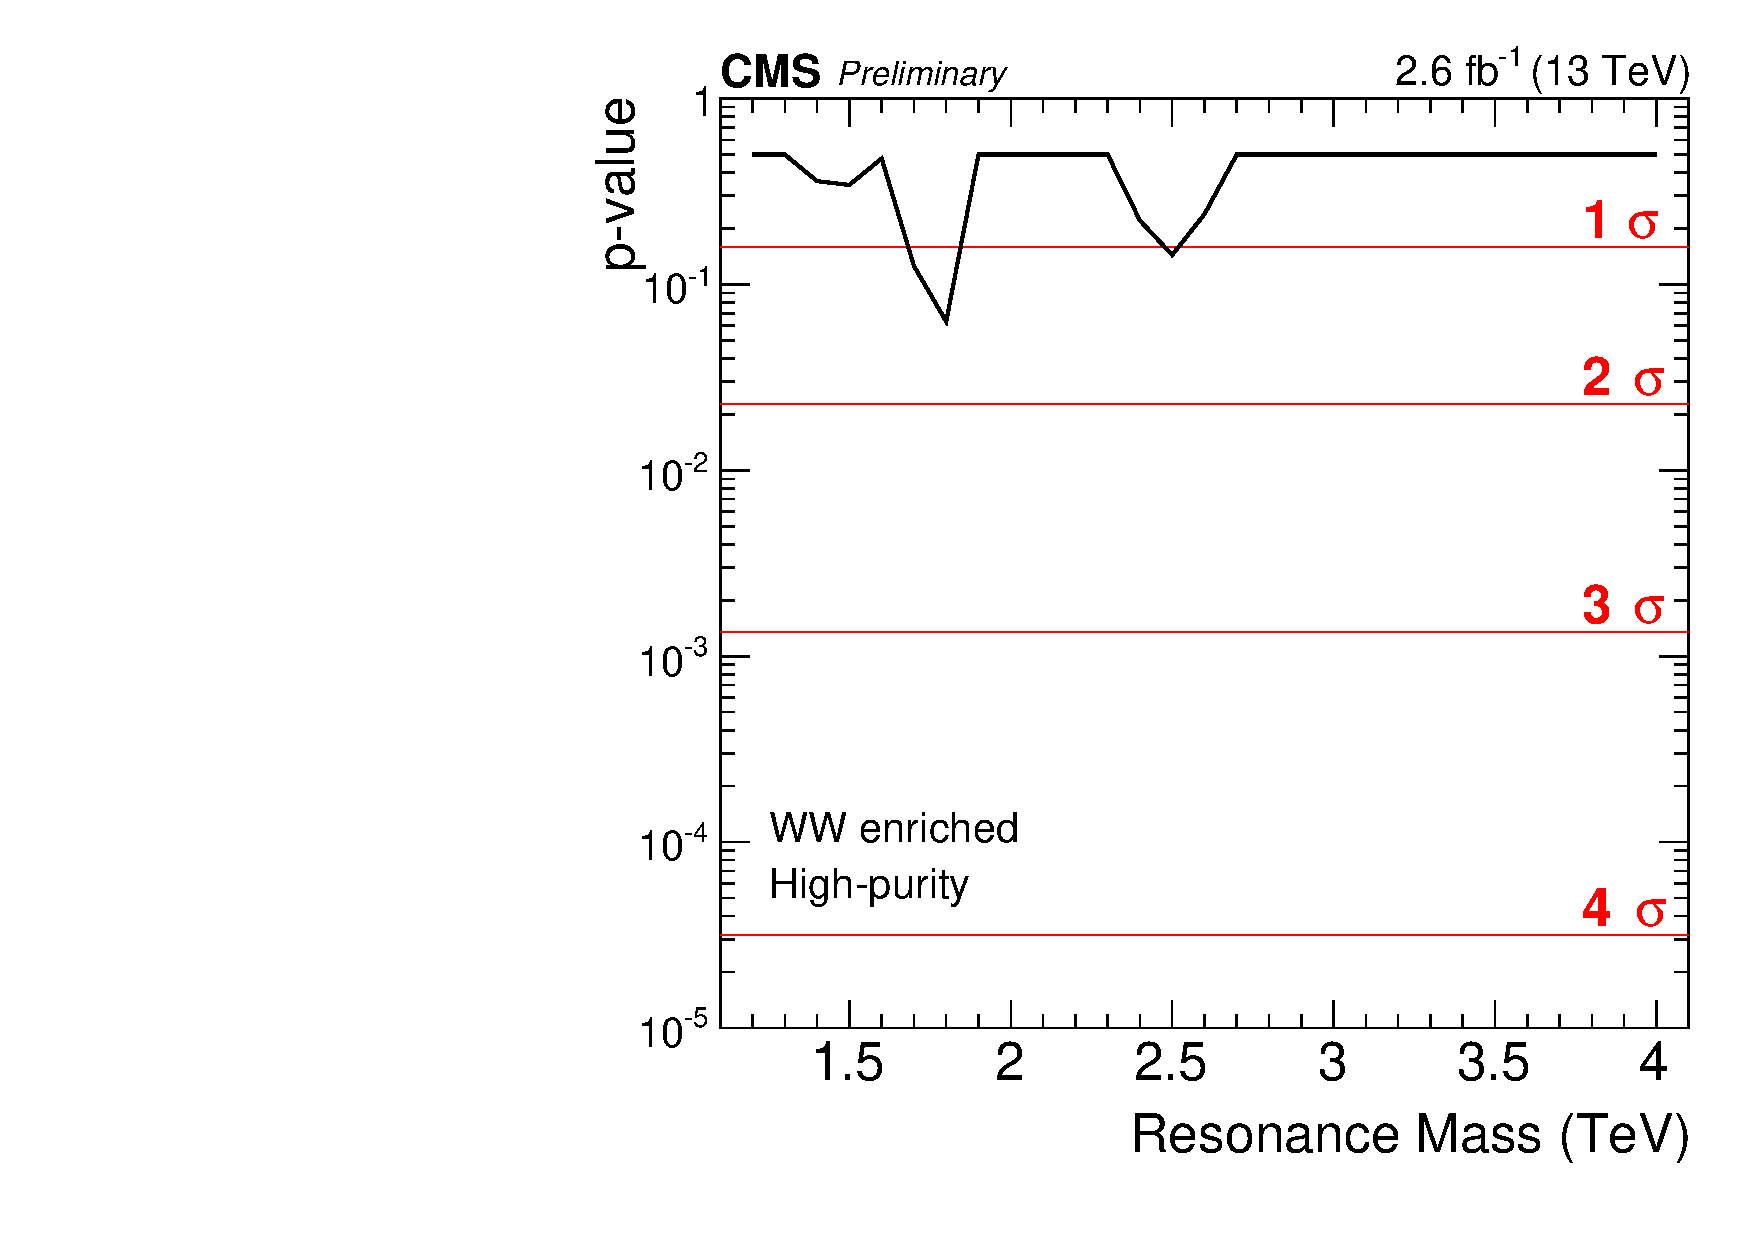
\includegraphics[width=0.327\textwidth]{figures/analysis/search1/AN-15-211/pvalues/pvalue_WZinWW_high_purity.pdf}
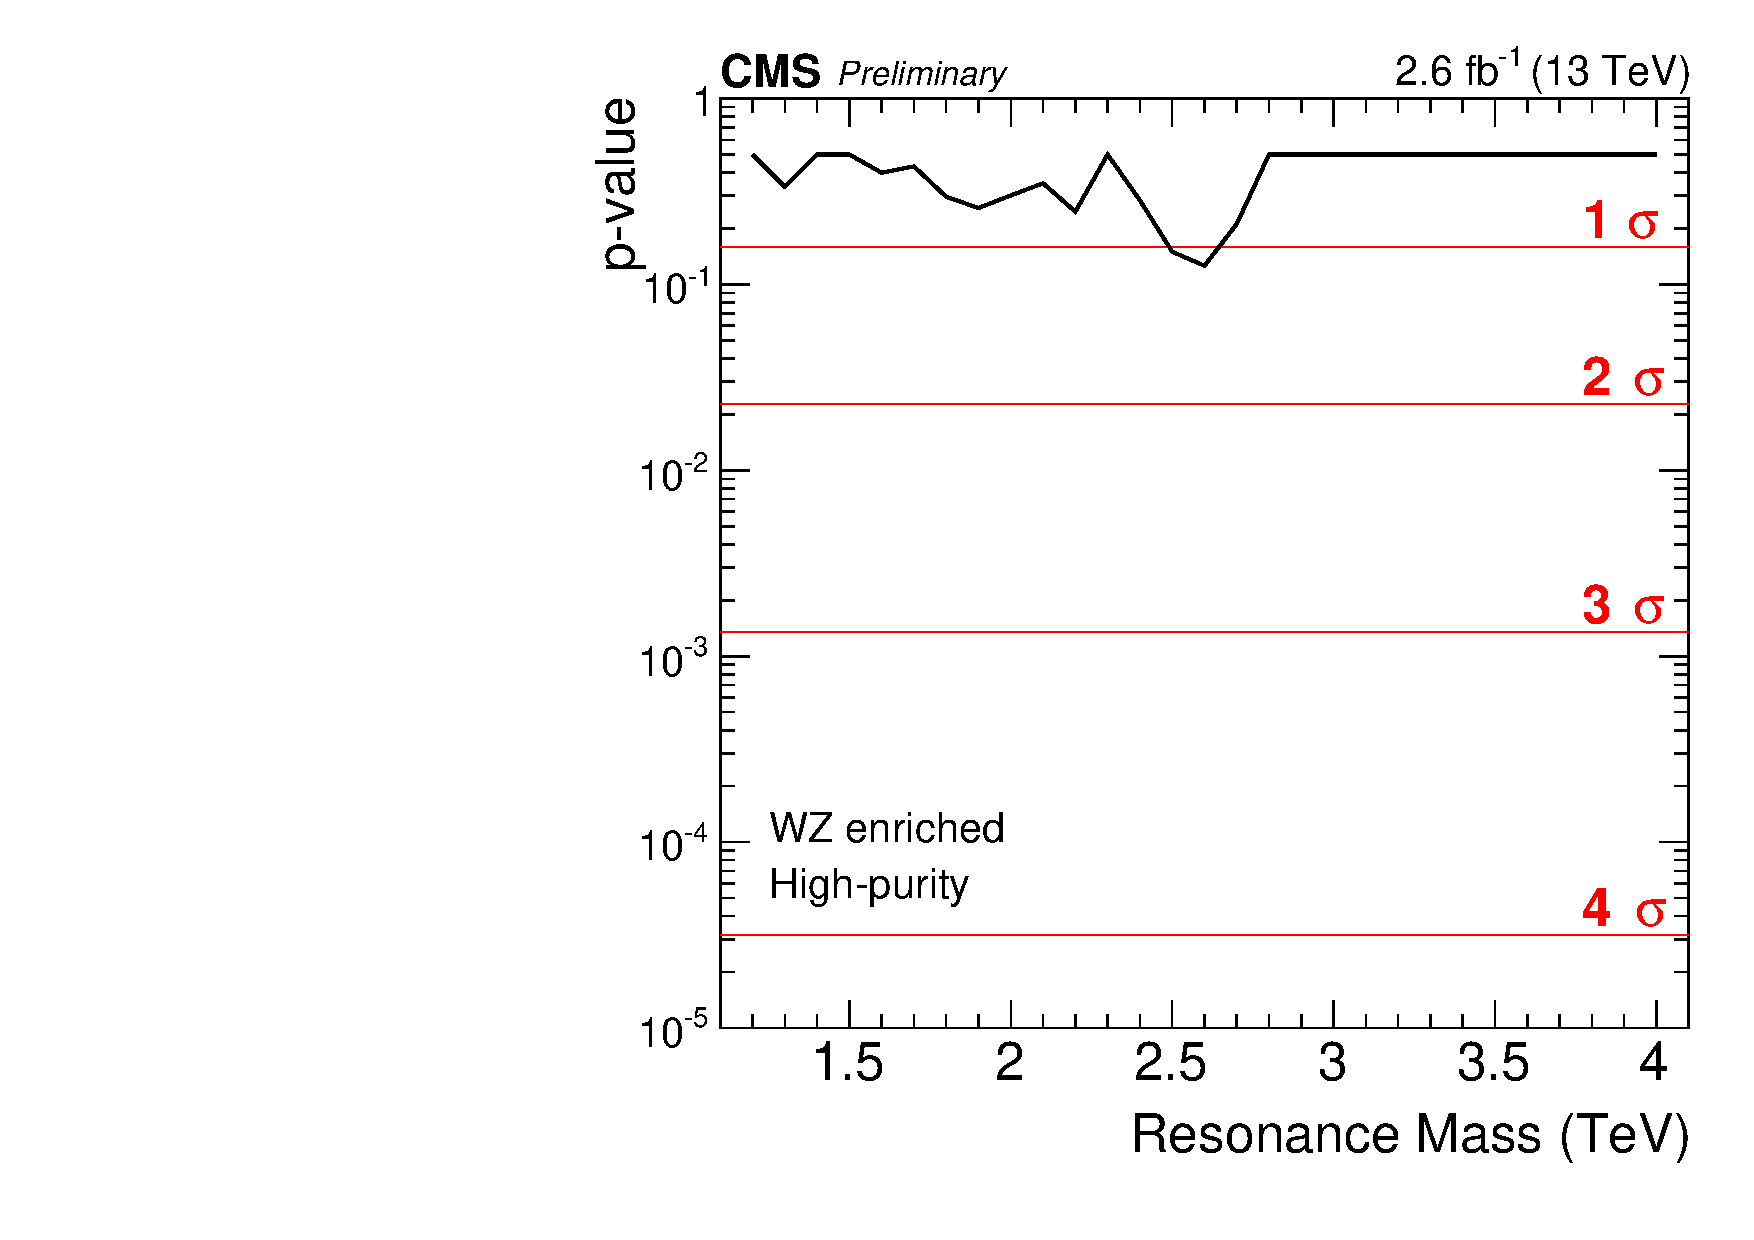
\includegraphics[width=0.327\textwidth]{figures/analysis/search1/AN-15-211/pvalues/pvalue_WZinWZ_high_purity.pdf}
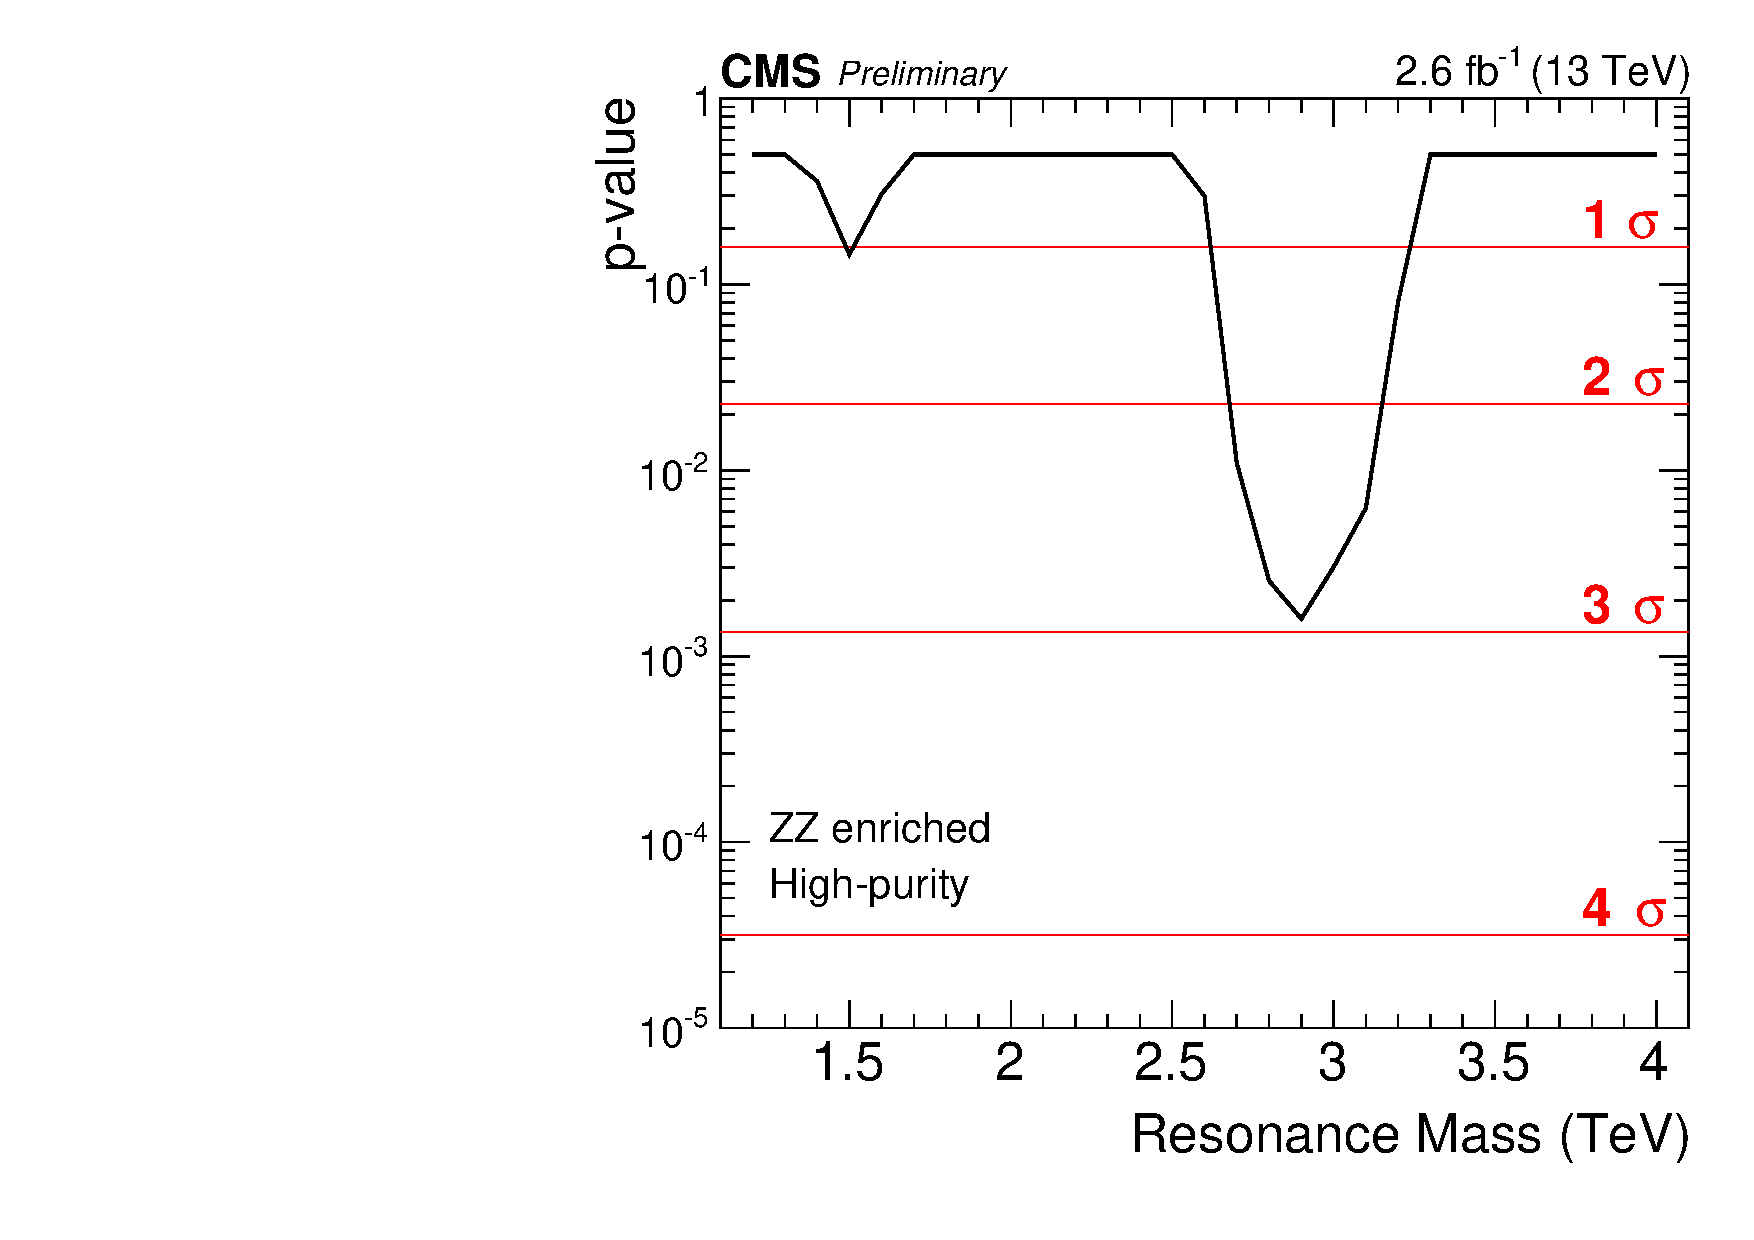
\includegraphics[width=0.327\textwidth]{figures/analysis/search1/AN-15-211/pvalues/pvalue_WZinZZ_high_purity.pdf}
\caption{Expected and observed limits at 95\% CL and corresponding p-values obtained in the different mass categories. Here for a $W'\rightarrow WZ$ signal in the high-purity category.}
\label{fig:app:Limits_HPWZ}
\end{figure}
\begin{figure}[h!]
\centering
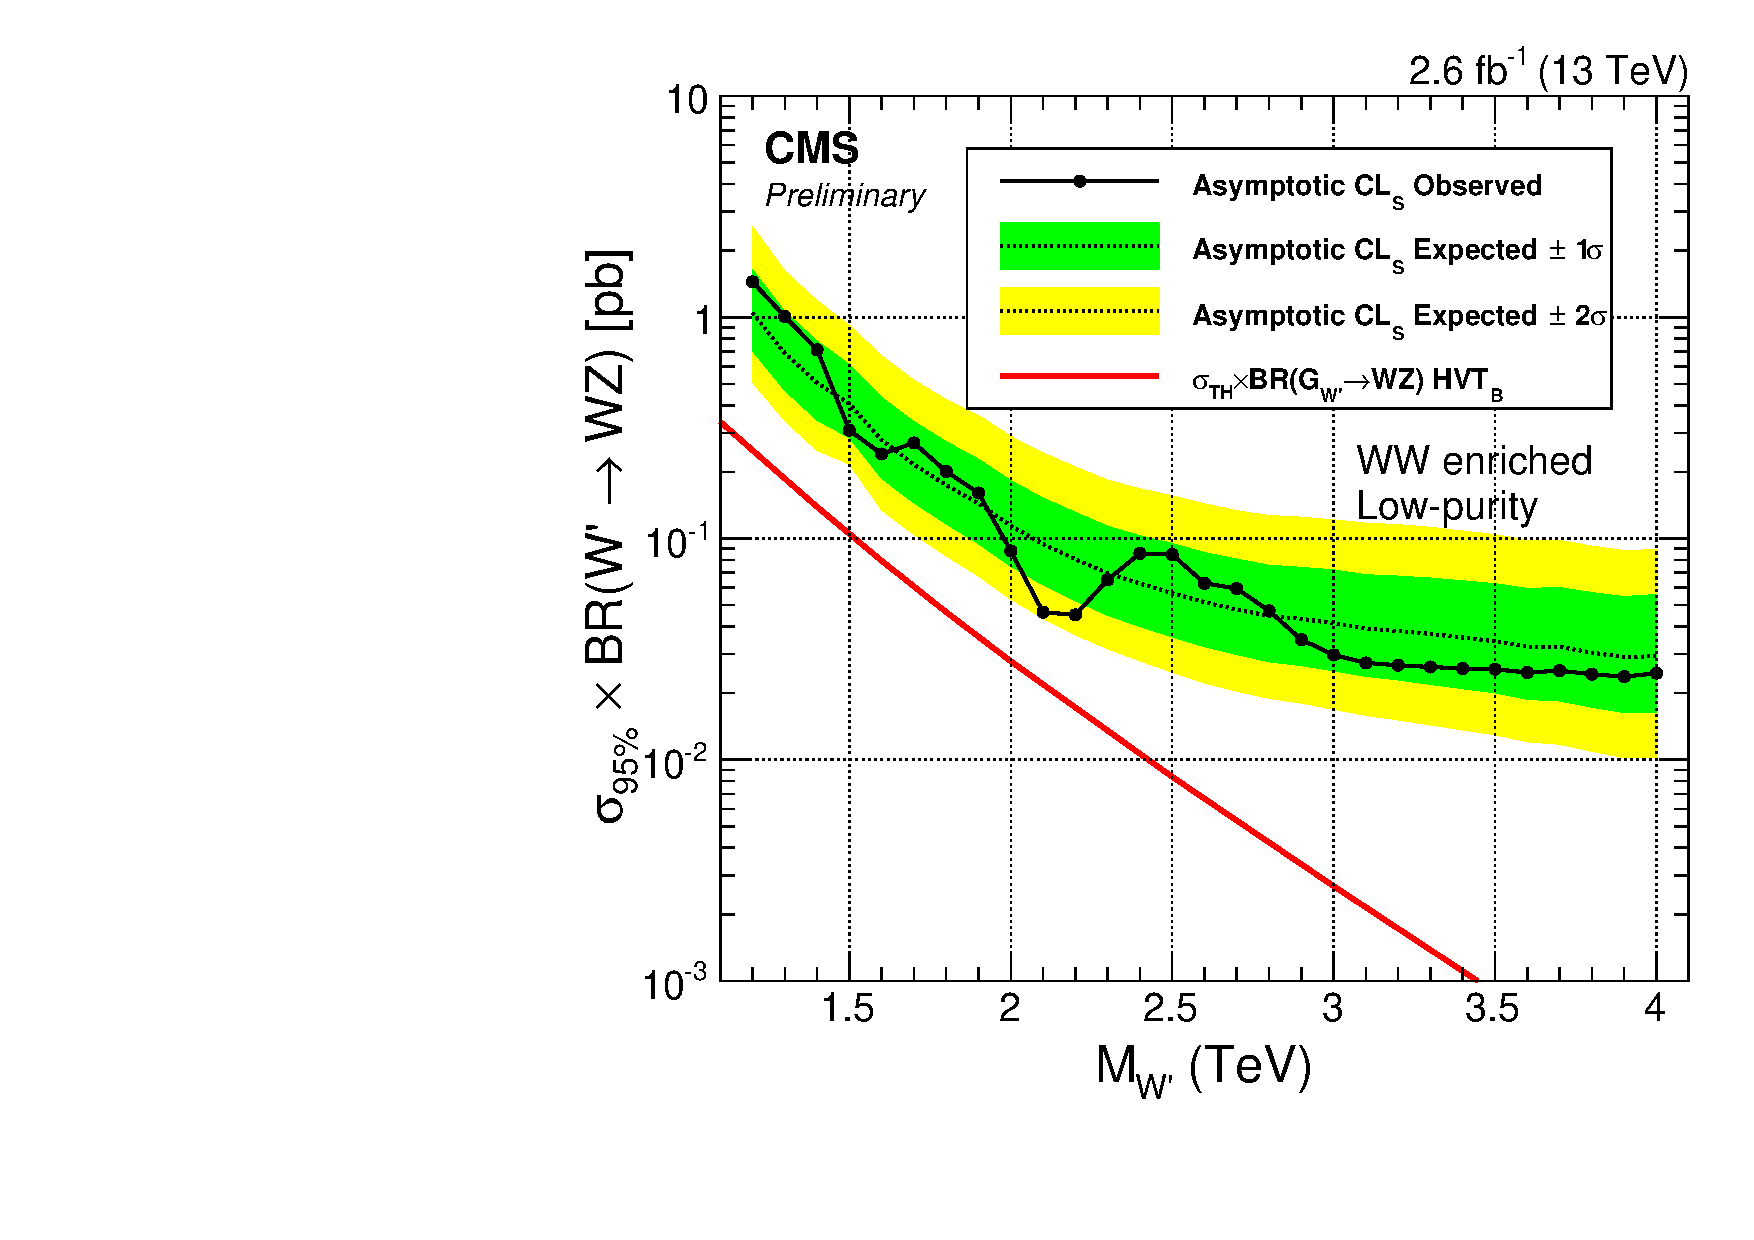
\includegraphics[width=0.327\textwidth]{figures/analysis/search1/AN-15-211/limits/brazilianFlag_WZ_WWLP_13TeV_wPDF.pdf}
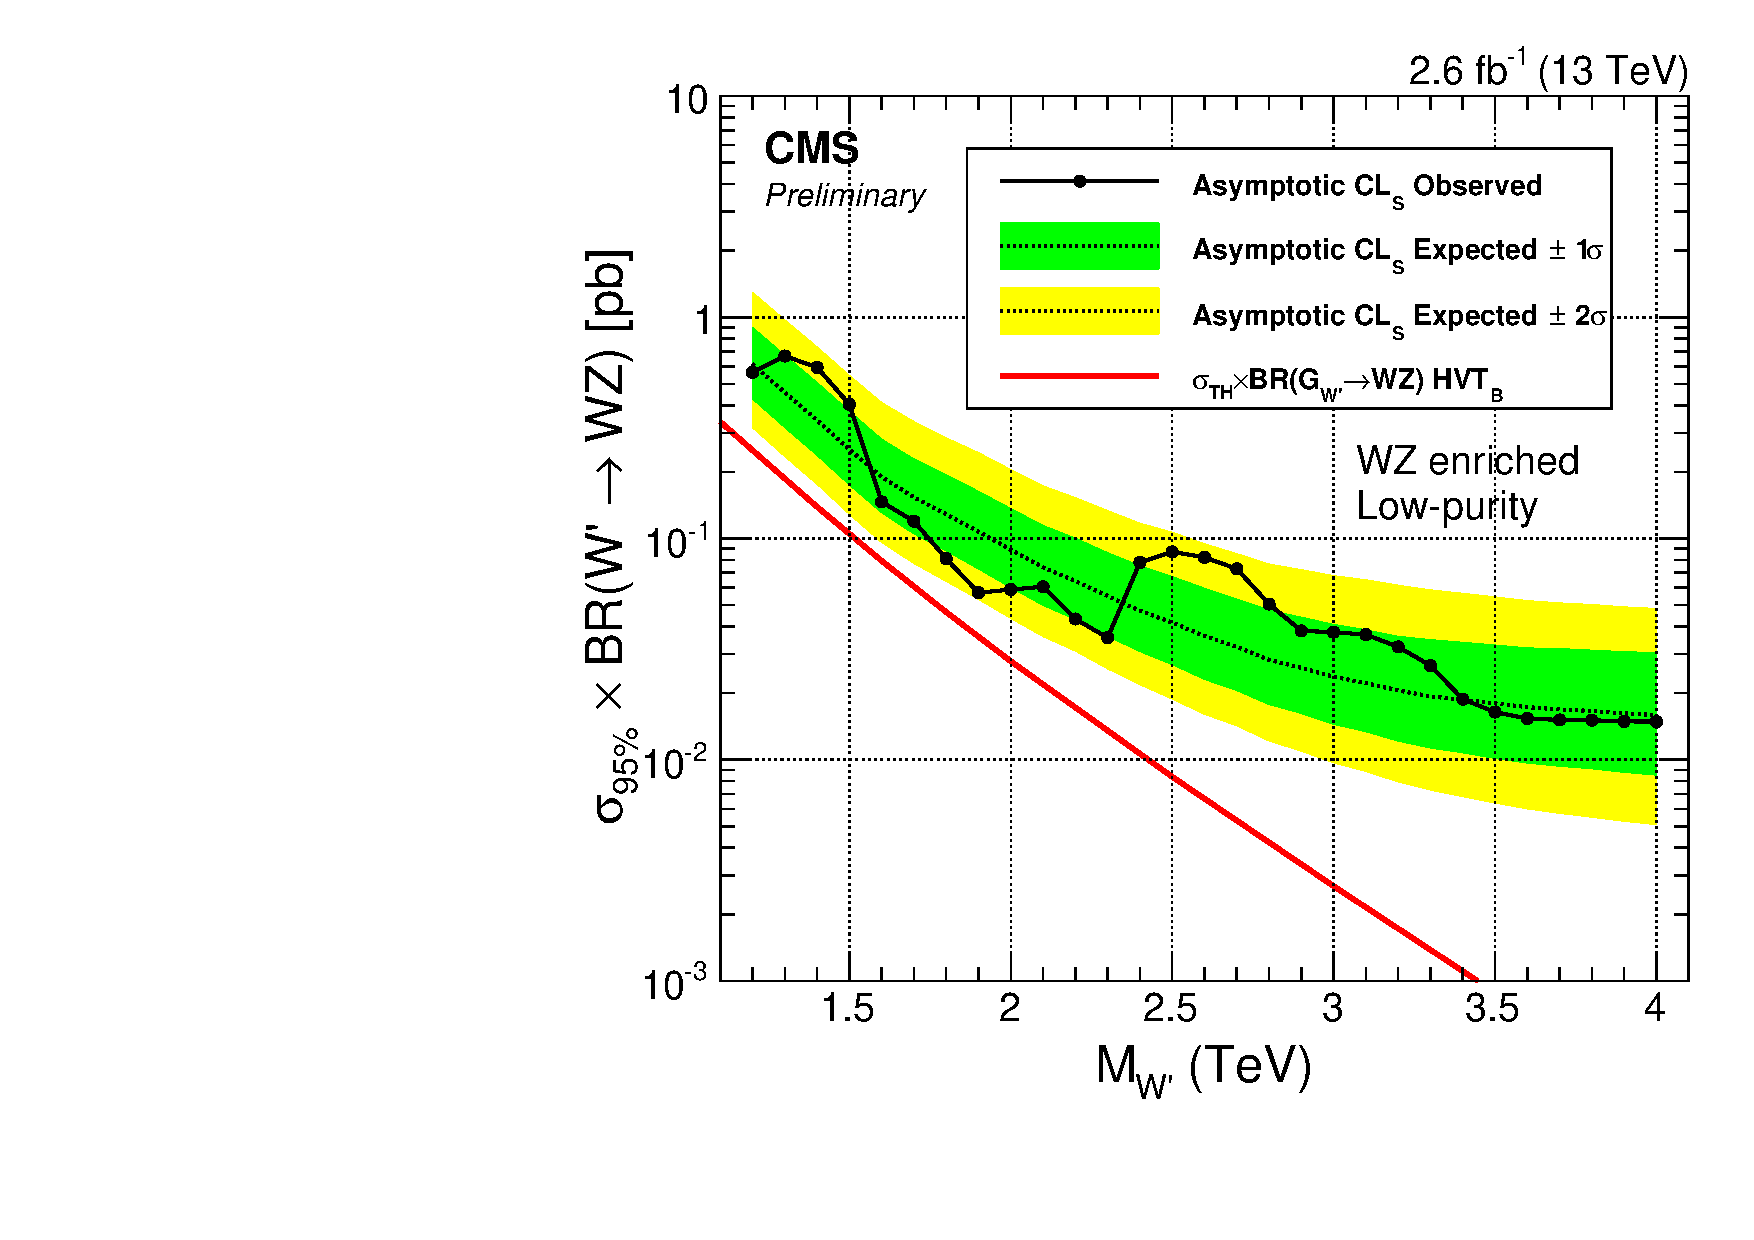
\includegraphics[width=0.327\textwidth]{figures/analysis/search1/AN-15-211/limits/brazilianFlag_WZ_WZLP_13TeV_wPDF.pdf}
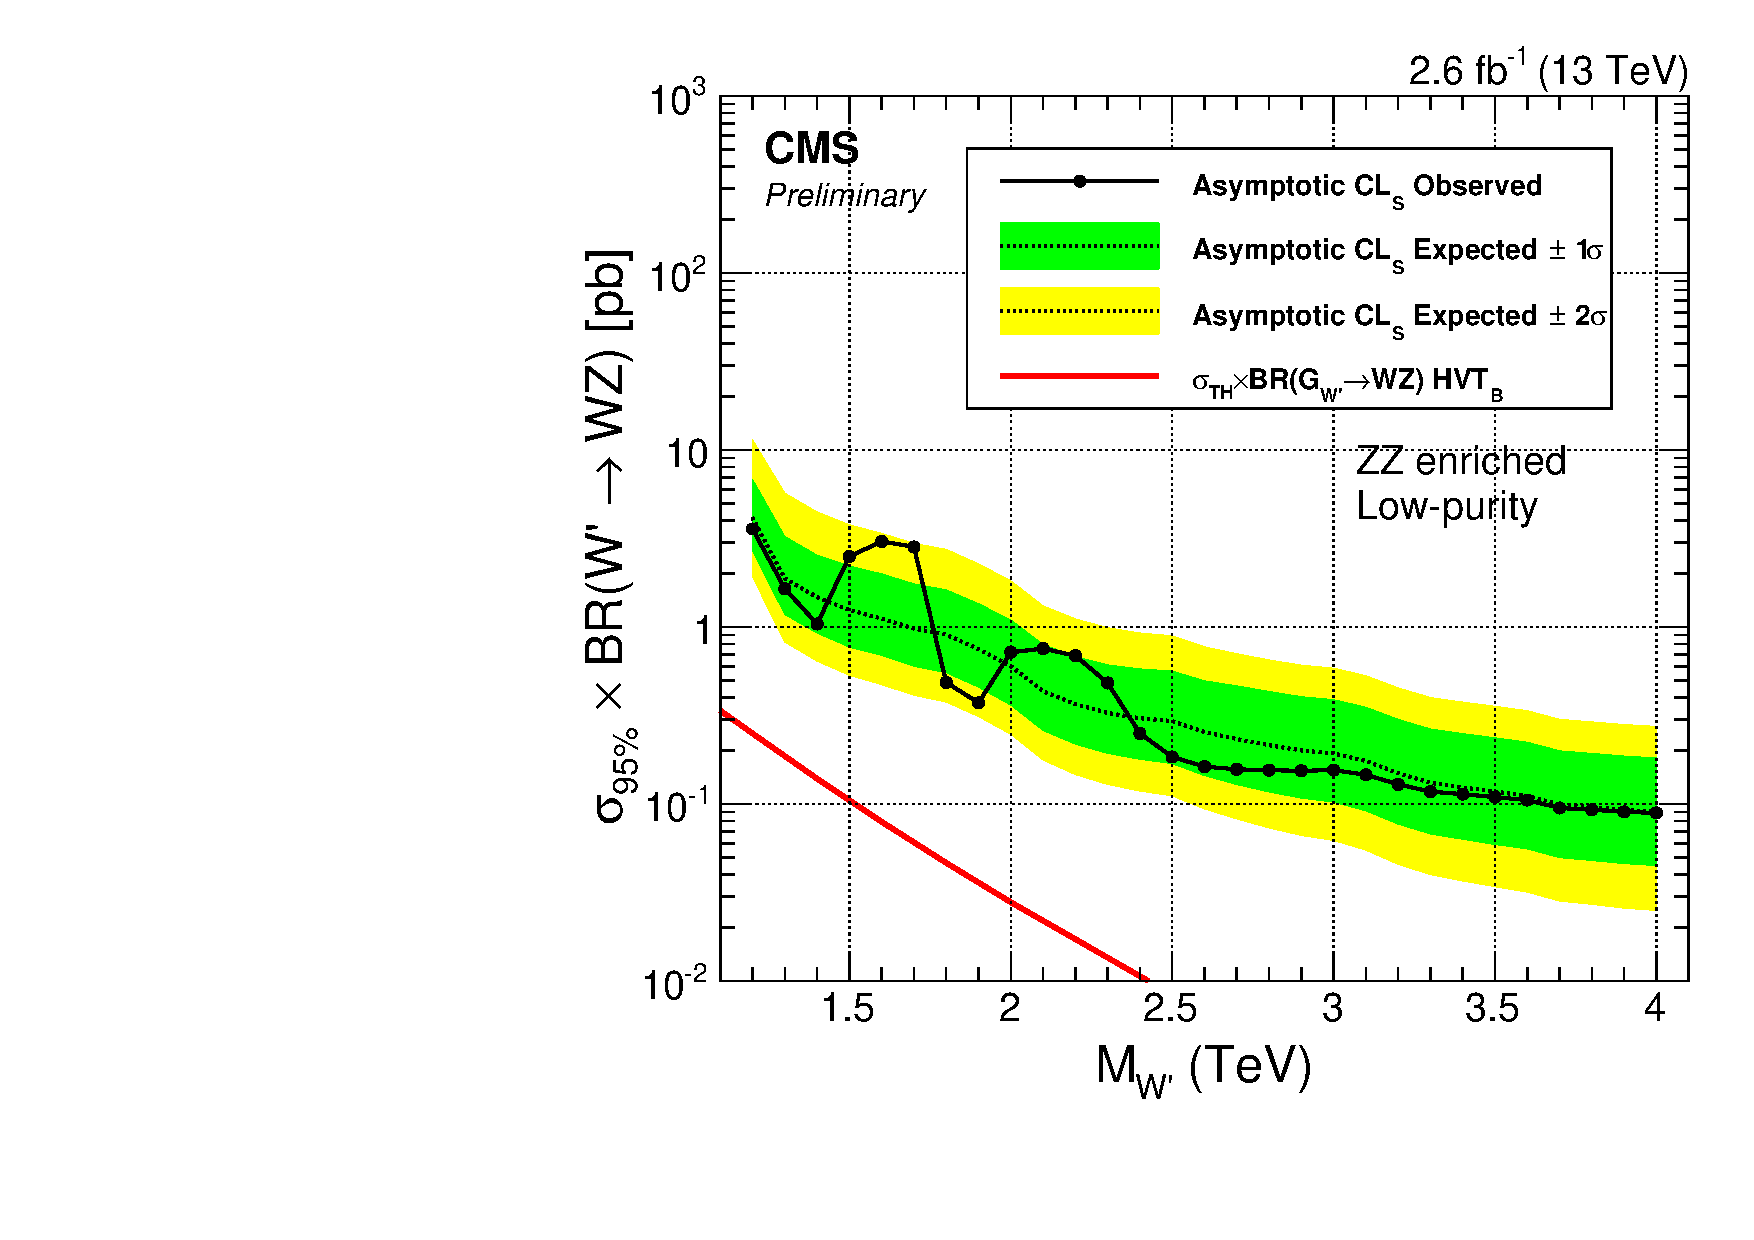
\includegraphics[width=0.327\textwidth]{figures/analysis/search1/AN-15-211/limits/brazilianFlag_WZ_ZZLP_13TeV_wPDF.pdf}\\
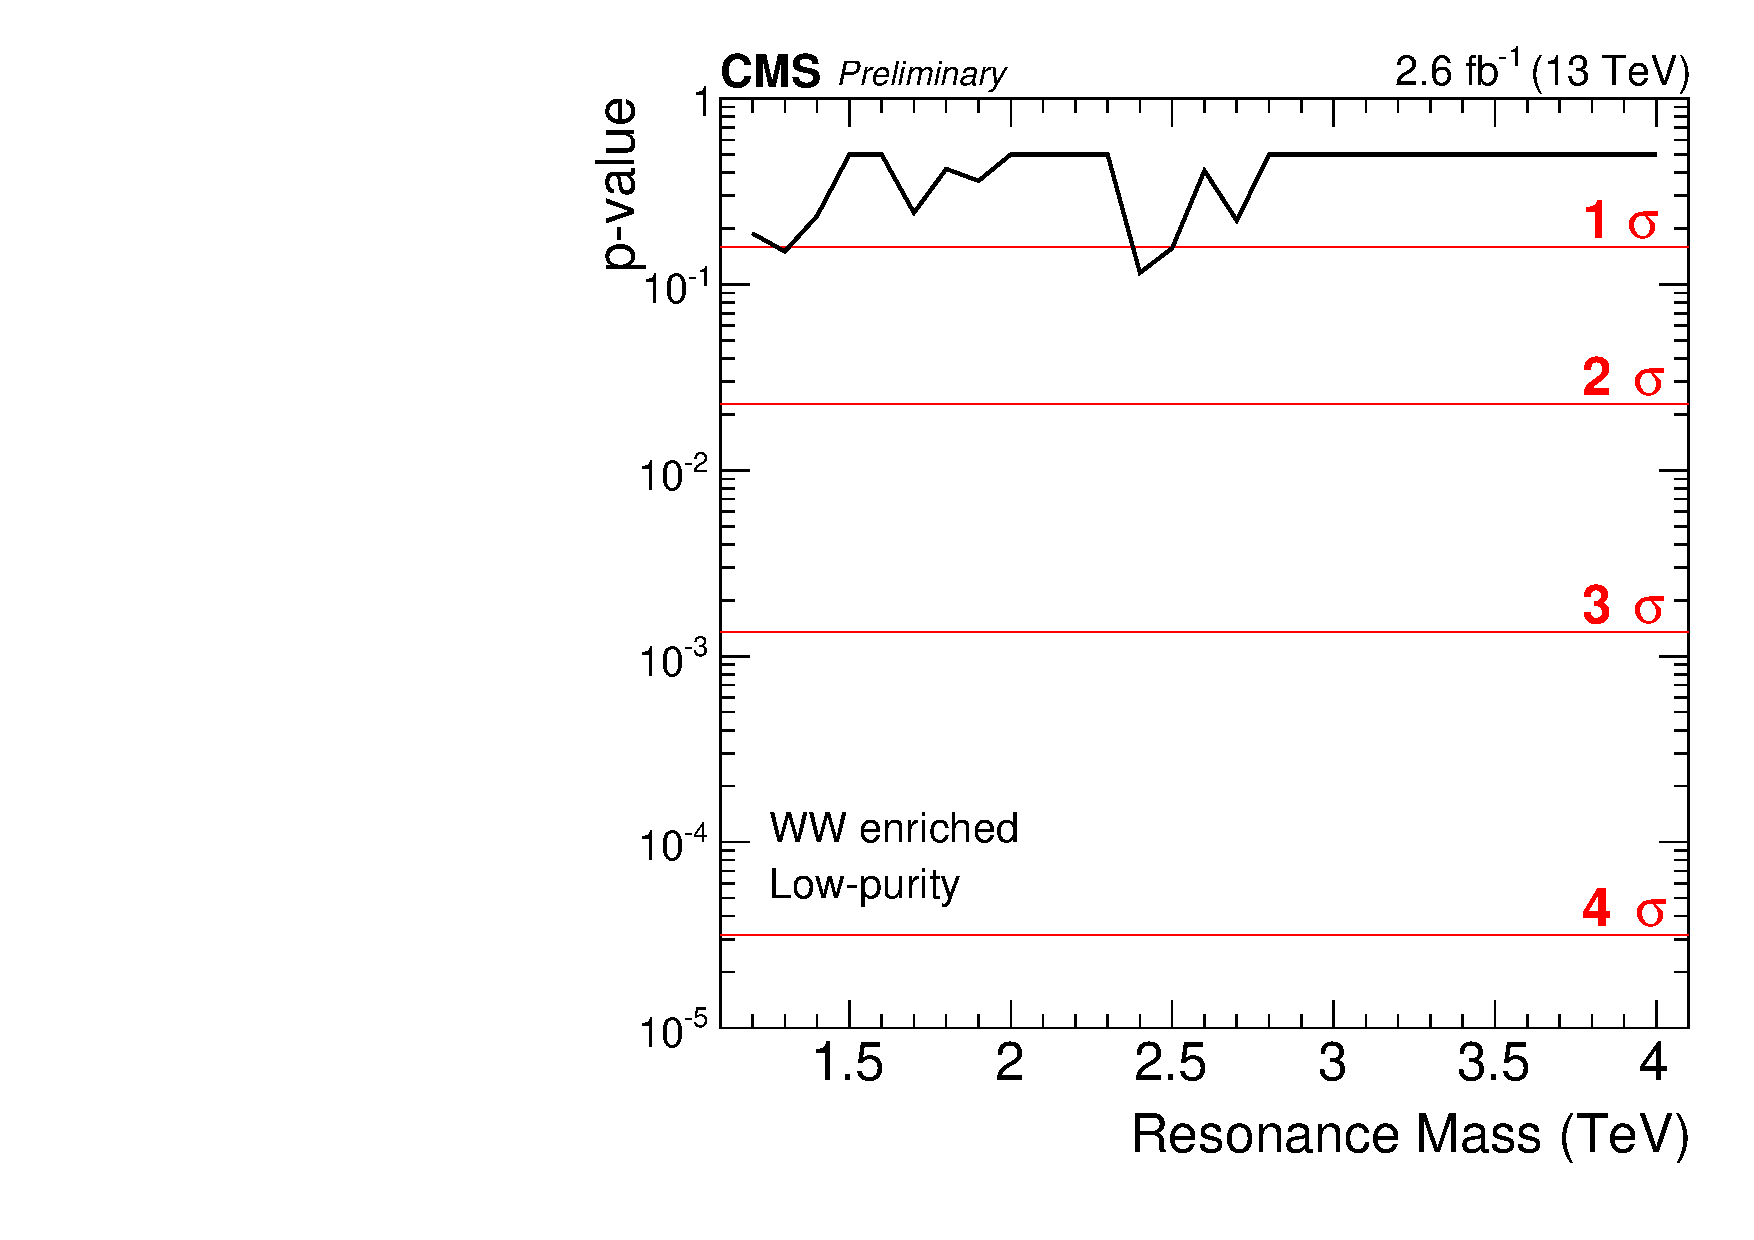
\includegraphics[width=0.327\textwidth]{figures/analysis/search1/AN-15-211/pvalues/pvalue_WZinWW_low_purity.pdf}
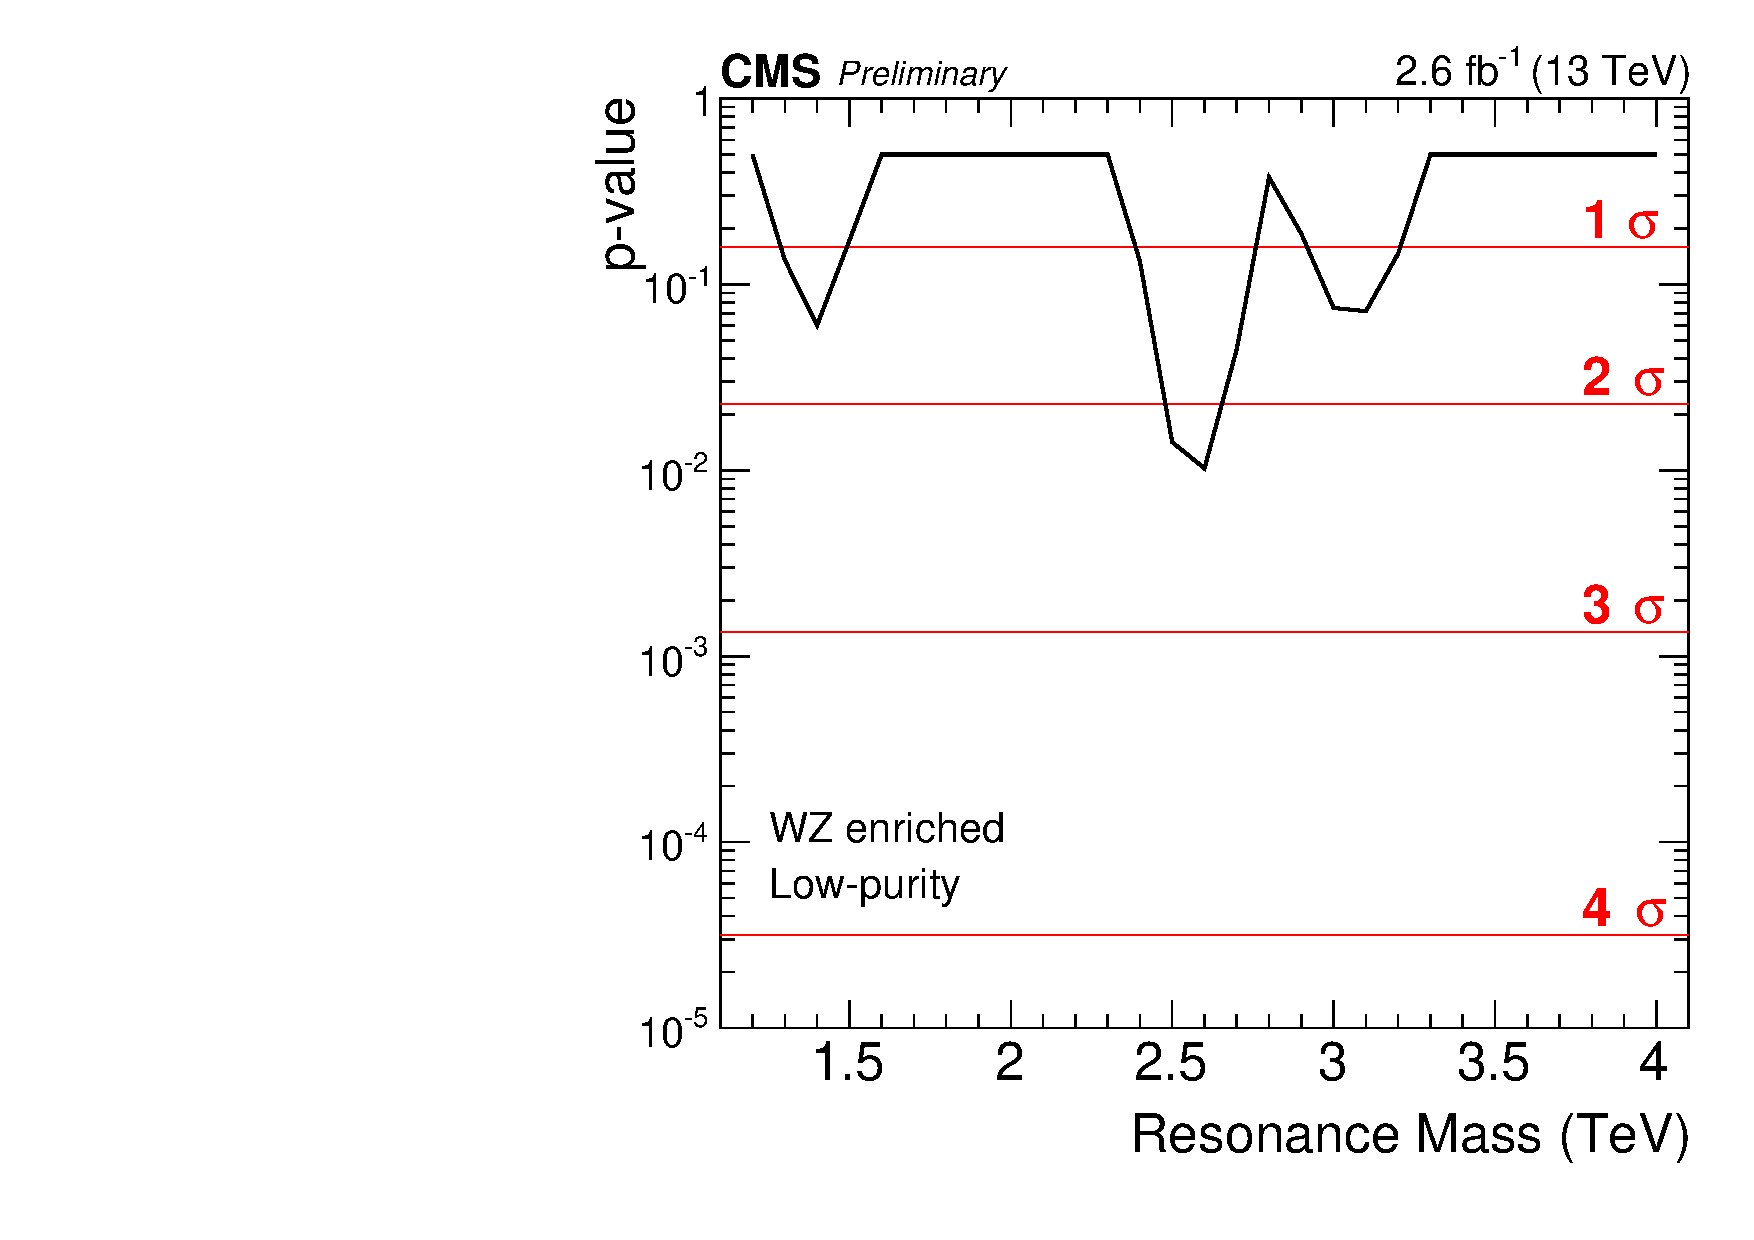
\includegraphics[width=0.327\textwidth]{figures/analysis/search1/AN-15-211/pvalues/pvalue_WZinWZ_low_purity.pdf}
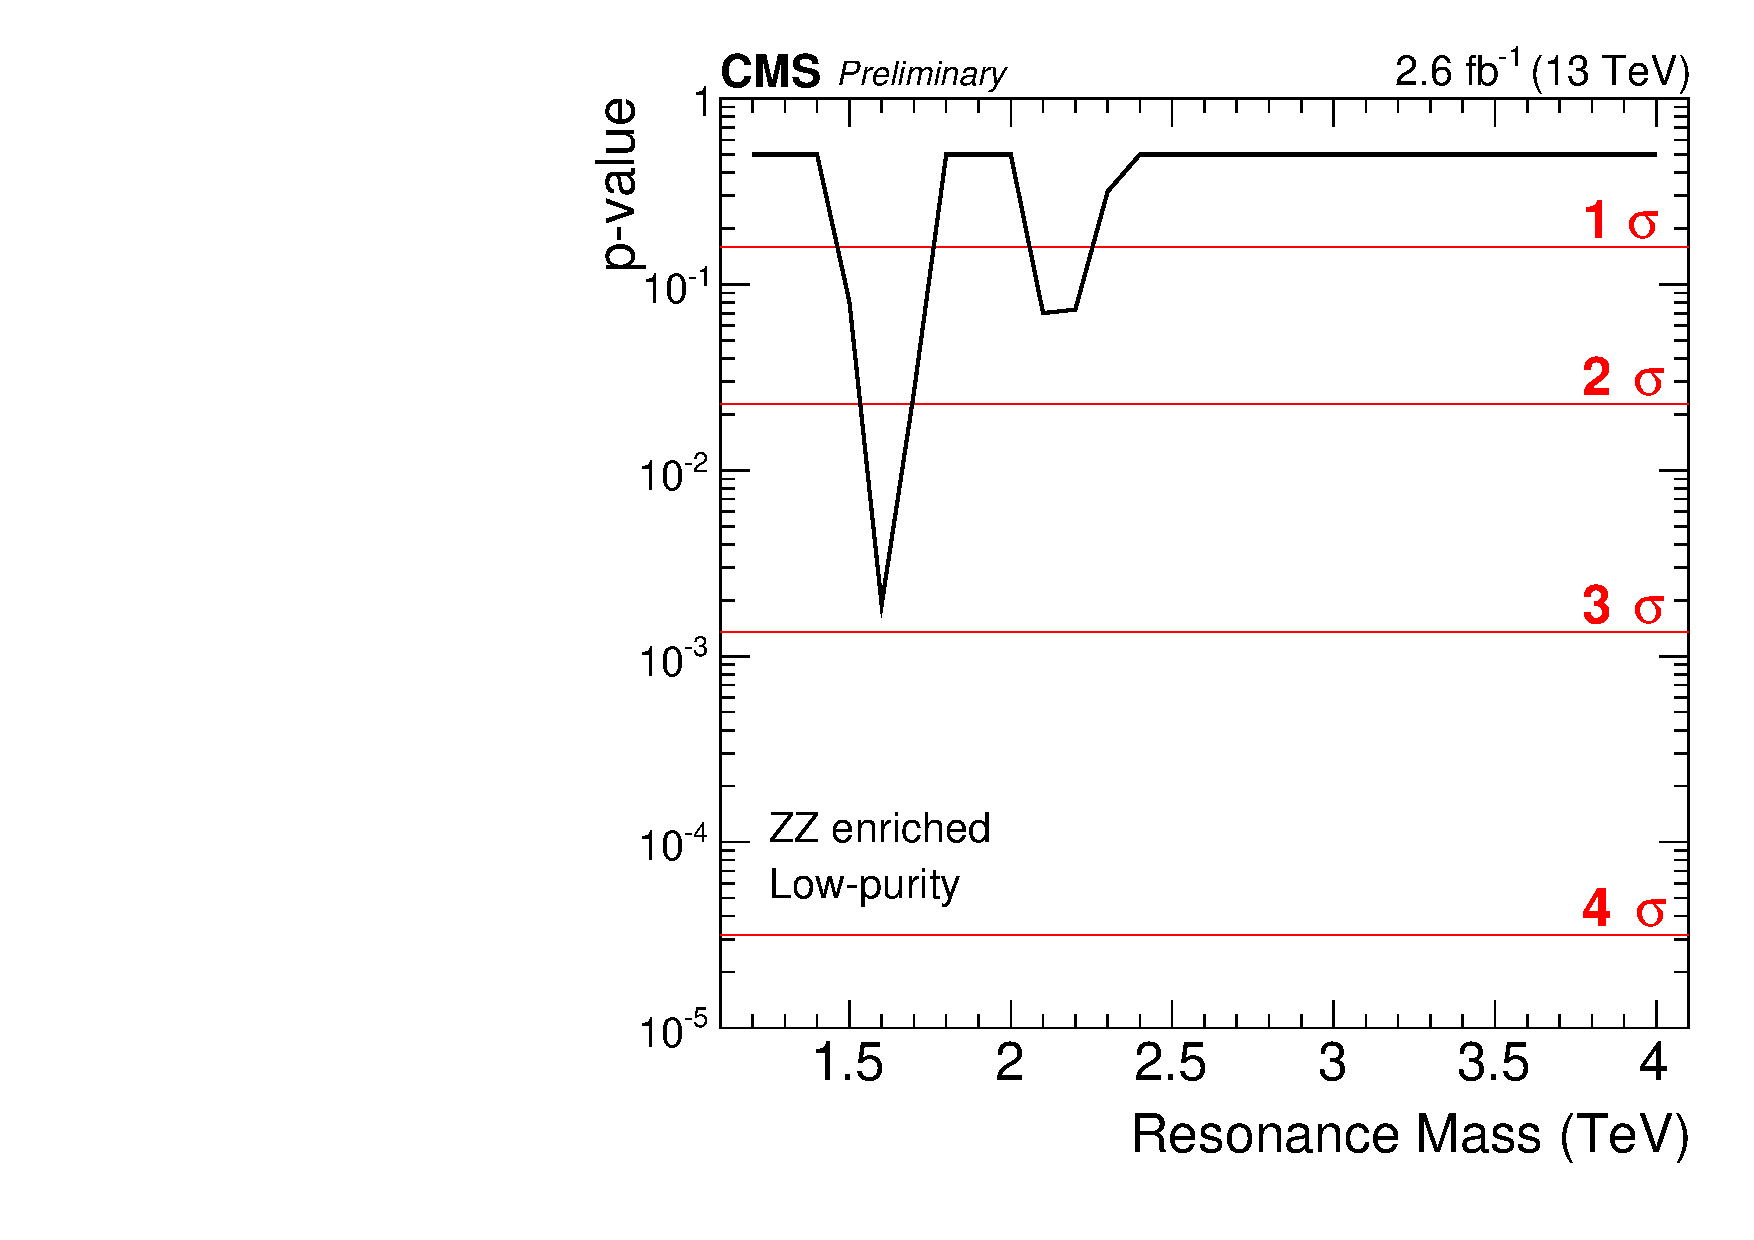
\includegraphics[width=0.327\textwidth]{figures/analysis/search1/AN-15-211/pvalues/pvalue_WZinZZ_low_purity.pdf}
\caption{Expected and observed limits at 95\% CL and corresponding p-values obtained in the different mass categories. Here for a $W'\rightarrow WZ$ signal in the low purity category.}
\label{fig:app:Limits_LPWZ}
\end{figure}
\begin{figure}[h!]
\centering
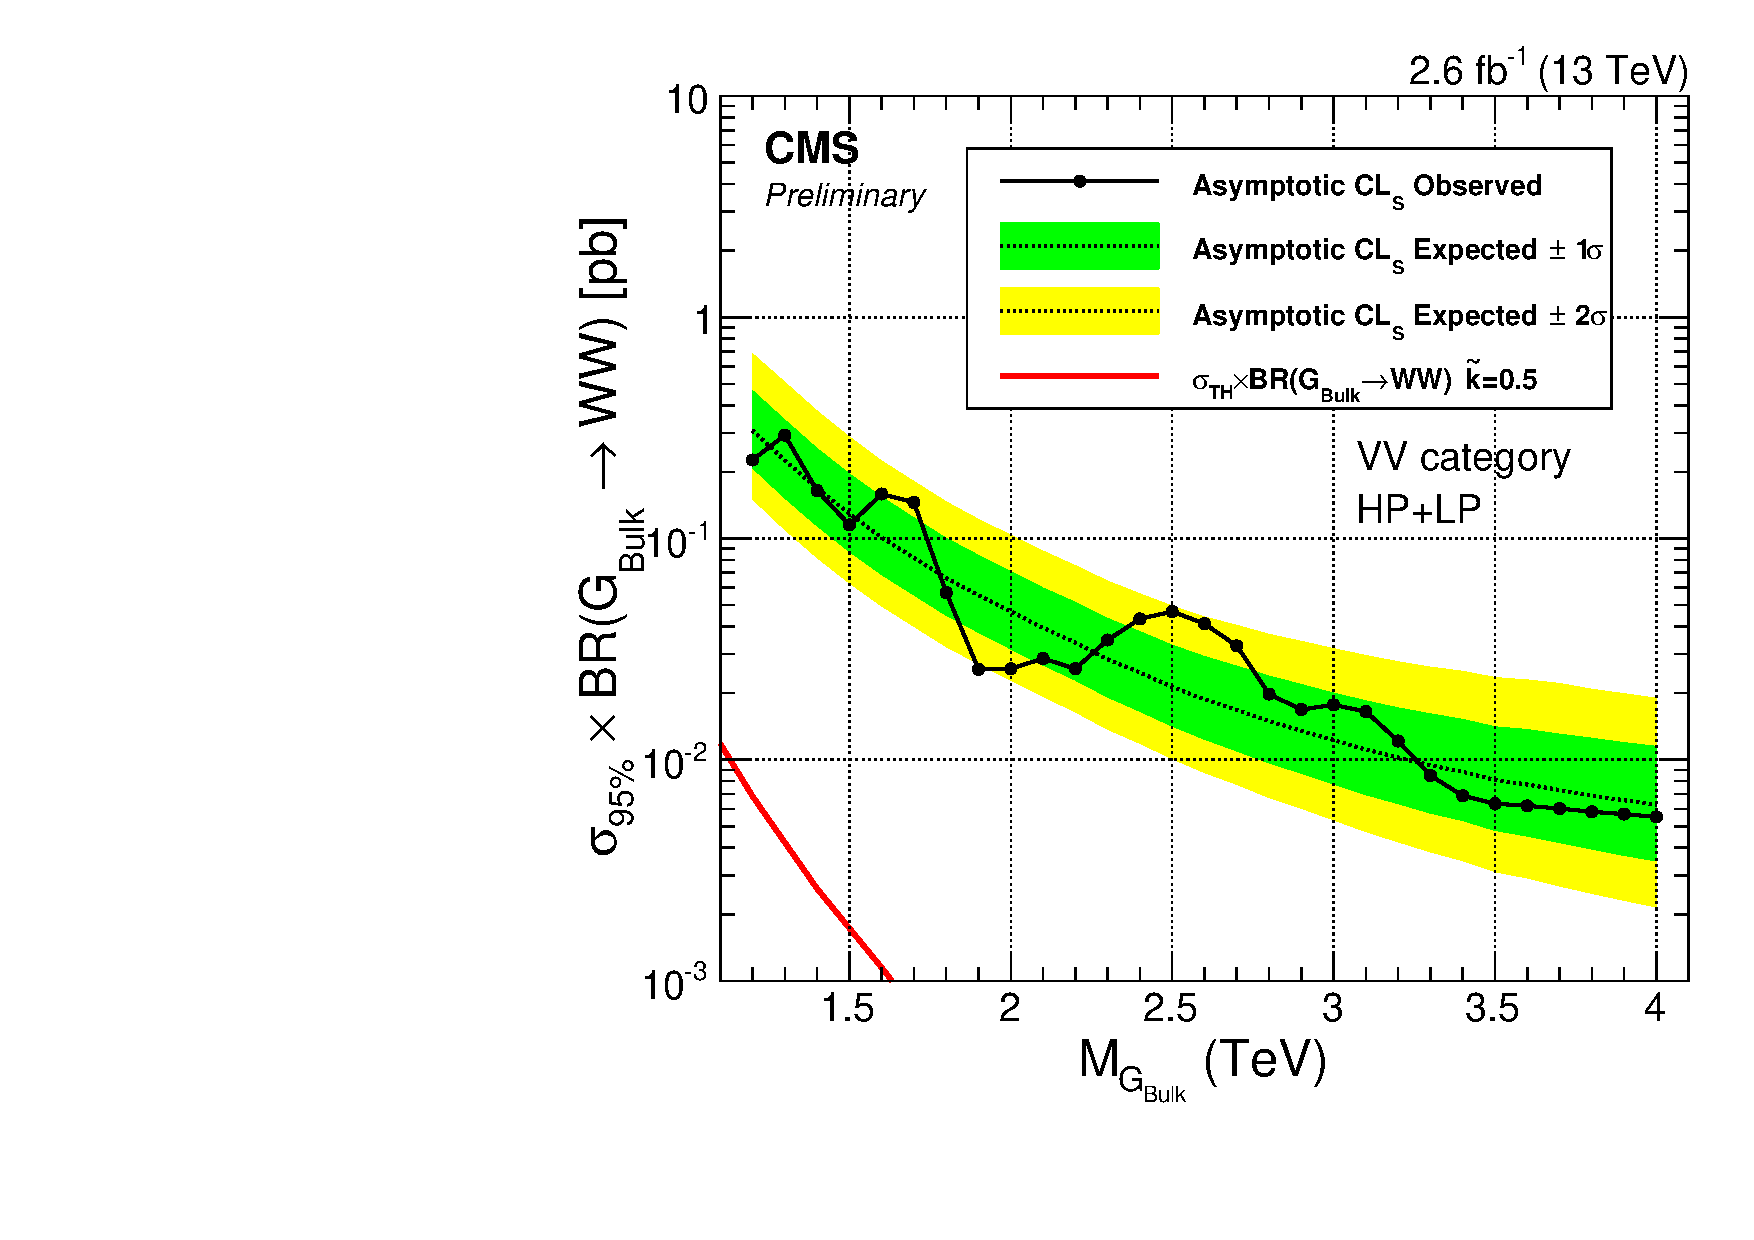
\includegraphics[width=0.327\textwidth]{figures/analysis/search1/AN-15-211/limits/brazilianFlag_BulkWW_old_combined_13TeV_wPDF.pdf}
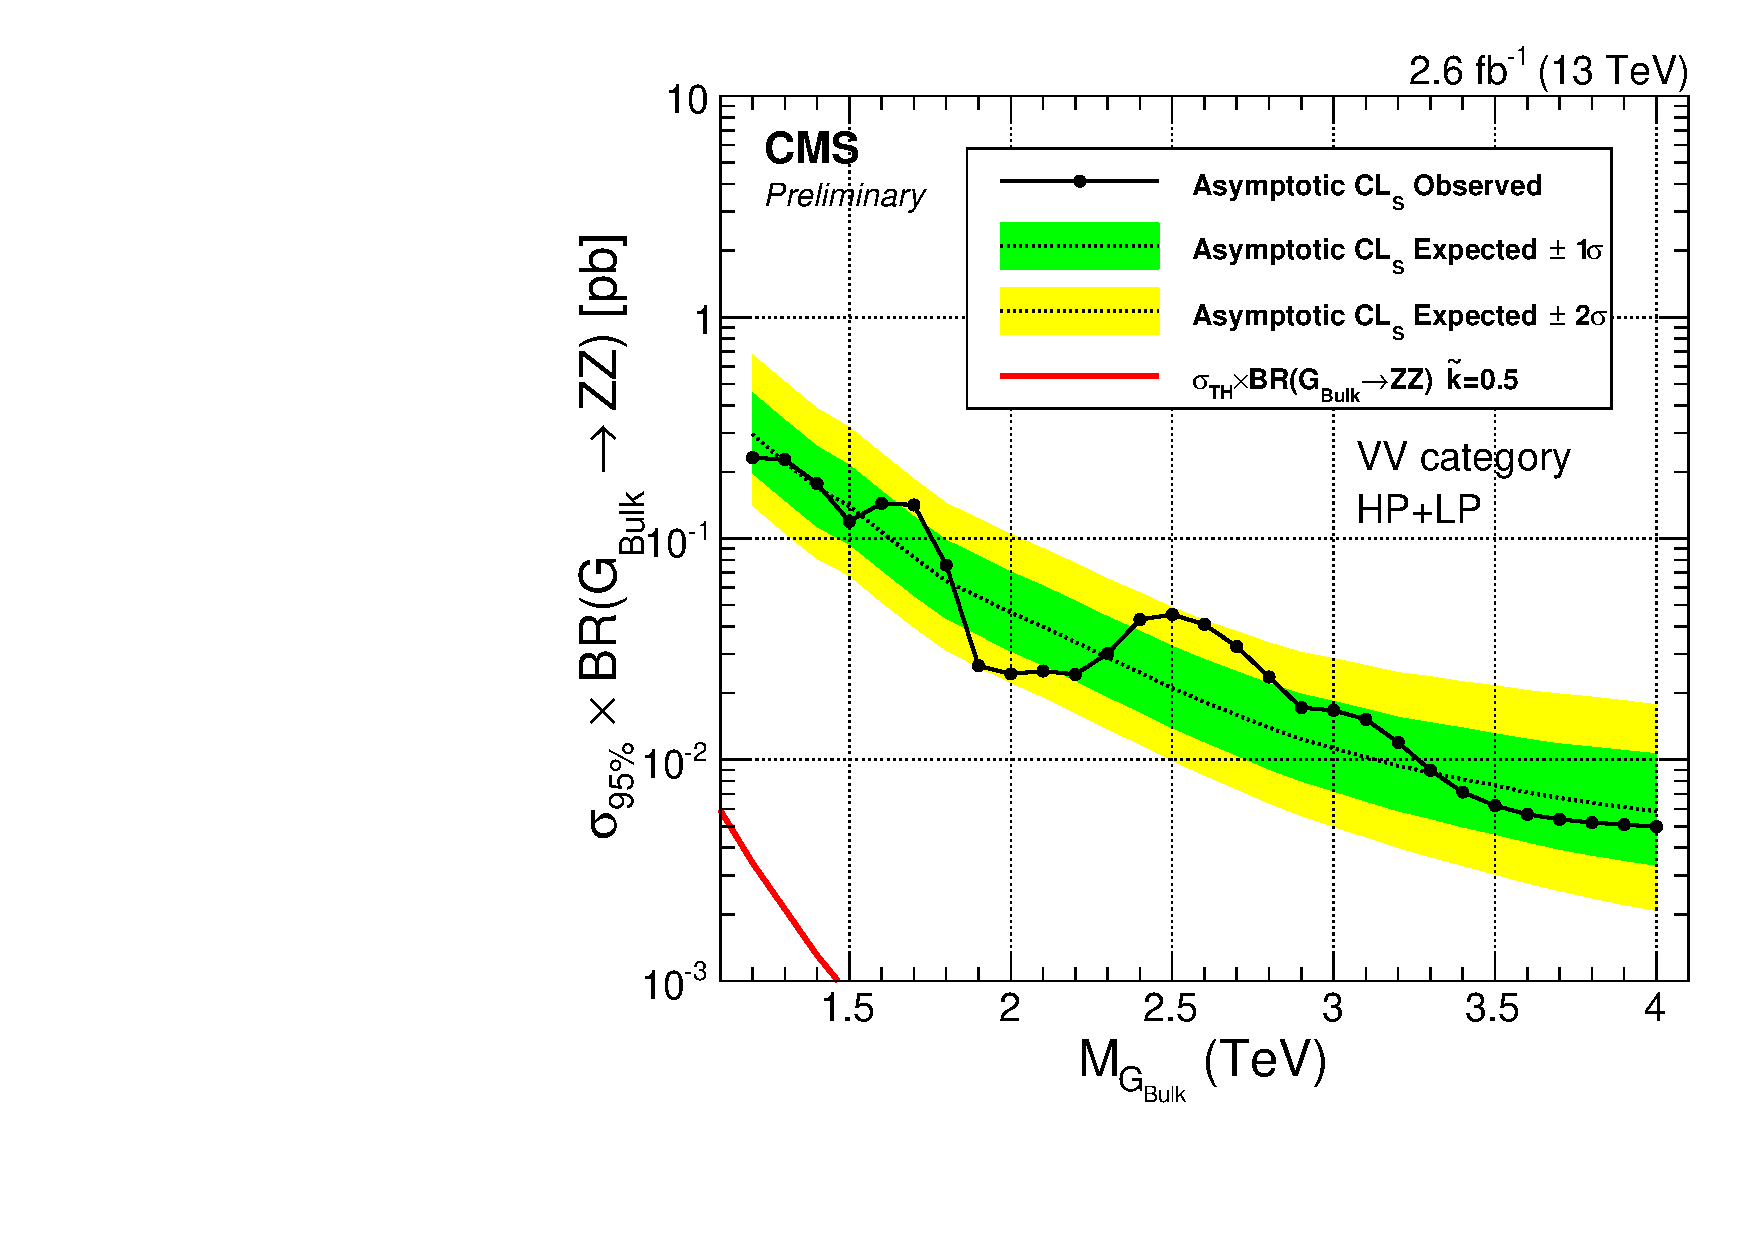
\includegraphics[width=0.327\textwidth]{figures/analysis/search1/AN-15-211/limits/brazilianFlag_BulkZZ_old_combined_13TeV_wPDF.pdf}
\includegraphics[width=0.327\textwidth]{figures/analysis/search1/AN-15-211/limits/brazilianFlag_WZ_old_combined_13TeV_wPDF.pdf}\\
\includegraphics[width=0.327\textwidth]{figures/analysis/search1/AN-15-211/pvalues/pvalue_BulkWWin_combined_old.pdf}
\includegraphics[width=0.327\textwidth]{figures/analysis/search1/AN-15-211/pvalues/pvalue_BulkZZin_combined_old.pdf}
\includegraphics[width=0.327\textwidth]{figures/analysis/search1/AN-15-211/pvalues/pvalue_WZin_combined_old.pdf}
\caption{Expected and observed limits at 95\% CL and corresponding obtained without splitting into mass categories. This analysis is performed as a cross check analysis and directly compares with the method used in the corresponding Run 1 analysis.  Here for a Bulk $G\rightarrow WW$ (left), $G\rightarrow ZZ$ (middle) and $W'\rightarrow WZ$ signal (right).}
\label{fig:app:Limits_CombOld}
\end{figure}
\clearpage

\chapter{Search II}
\vspace*{\fill}\newpage
\section{mMDT and underlying event}
\label{app:sdue}
Signal jets groomed with mMDT using a $y_{cut}$ definition, $min(p^2_{T,s_1}, p^2_{T,s_2})\Delta R(s_1,s_2)/m^2_{j} > y_{cut}$, rather than a $z_{cut}$ definition (as is default in CMS), $\frac{ \textrm{min}(p_{T,i},p_{T,j}) }{ p_{T,P} } > z_{cut} $, were found to be far more sensitive to the underlying event than pruned jets~\cite{Dasgupta:2015yua}. Figure~\ref{fig:searchII:ue} shows the signal efficiency for pruning (left) and softdrop (right) as a function of jet transverse momenta when including final state radiation (FSR) only, final and initial state radiation (ISR), hadronization, and hadronization with an underlying event component added.
\begin{figure}[h!]
\centering
\includegraphics[width=0.79\textwidth]{figures/analysis/search2/misc/pruningvssd_ue.pdf}
\caption{The signal efficiency for pruning (left) and softdrop (mMDT) (right) as a function of jet \PT when adding FSR, ISR, hadronization and UE. The UE has a severe impact on the softdrop efficiency for signal jets~\cite{Dasgupta:2015yua}. }
\label{fig:searchII:ue}
\end{figure}
At parton level, as well as after hadronization, the two algorithms perform very similar as a function of \PT. However, once UE contamination is added, the softdrop tagging efficiency is severely affected. This can be explained by the larger effective radius considered by the mMDT algorithm ( $\propto \mV/\PT \sqrt{z_{cut}(1-z_{cut})}$ ) in comparison to pruning ( $\propto \mV/\PT$ ), as can be seen from Equations~\ref{eq:softdrop} and \ref{eq:pruning}. This observation corresponds very well with the shift in jet mass we observed for softdrop as a function of \PT in Section~\ref{sec:searchI:wtagging}: as the jet \PT decreases, the mMDT effective radius increases and the jet mass mean shifts to higher values, due to absorbing more background radiation.
\clearpage
\section{W-tagging scale factor: Additional plots}
\label{app:sf16}
Figures~\ref{fig:app:ttfitsd} shows the \ttbar real \PW (top) and non-\PW (bottom) PUPPI softdrop jet mass distributions for jets that passed (left) and failed (right column) the N-subjettiness selections PUPPI
$\tau_{21}~<$~0.40.
\begin{figure}[h!]
  \centering
    \includegraphics[width=0.49\textwidth]{figures/vtagging/AN-16-215/plots_76X/fits_TTMC/plots_em_HP0v40powheg_76X_PuppiSD_MCfits/{_TTbar_realWExoDiBosonAnalysis.WWTree_TTbar_powheg_76X_GausErfExp_ttbar_with_pull}.pdf}
    \includegraphics[width=0.49\textwidth]{figures/vtagging/AN-16-215/plots_76X/fits_TTMC/plots_em_HP0v40powheg_76X_PuppiSD_MCfits/{_TTbar_realW_failtau2tau1cutExoDiBosonAnalysis.WWTree_TTbar_powheg_76X_GausErfExp_ttbar_failtau2tau1cut_with_pull}.pdf}\\
    \includegraphics[width=0.49\textwidth]{figures/vtagging/AN-16-215/plots_76X/fits_TTMC/plots_em_HP0v40powheg_76X_PuppiSD_MCfits/{_TTbar_fakeWExoDiBosonAnalysis.WWTree_TTbar_powheg_76X_ErfExp_ttbar_with_pull}.pdf}
    \includegraphics[width=0.49\textwidth]{figures/vtagging/AN-16-215/plots_76X/fits_TTMC/plots_em_HP0v40powheg_76X_PuppiSD_MCfits/{_TTbar_fakeW_failtau2tau1cutExoDiBosonAnalysis.WWTree_TTbar_powheg_76X_ErfExp_ttbar_failtau2tau1cut_with_pull}.pdf}
  \caption{Fit to the real \PW (top) and non-\PW (bottom) softdrop jet mass distribution for jets that pass (left) and fail (right) the cut on PUPPI $\tau_{21}~<$~0.4.}
  \label{fig:app:ttfitsd}
\end{figure}
Figures~\ref{fig:app:minorbkrsd} shows the fitted PUPPI softdrop jet mass distributions for the non-dominant backgrounds in the evaluation of the W-tagging scale factors. Here it is shown for jets that pass (top) and failed (bottom) the N-subjettiness selections PUPPI
$\tau_{21}~<$~0.40.
\begin{figure}[h!]
   \centering
    \includegraphics[width=0.30\textwidth]{figures/vtagging/AN-16-215/{_STopExoDiBosonAnalysis.WWTree_STop_76X_ErfExpGaus_sp}.pdf}
    \includegraphics[width=0.30\textwidth]{figures/vtagging/AN-16-215/{_WJets0ExoDiBosonAnalysis.WWTree_WJets_76X_ErfExp}.pdf}
    \includegraphics[width=0.30\textwidth]{figures/vtagging/AN-16-215/{_VVExoDiBosonAnalysis.WWTree_VV_76X_ExpGaus}.pdf}\\
    \includegraphics[width=0.30\textwidth]{figures/vtagging/AN-16-215/{_STop_failtau2tau1cutExoDiBosonAnalysis.WWTree_STop_76X_ErfExpGaus_sp}.pdf}
    \includegraphics[width=0.30\textwidth]{figures/vtagging/AN-16-215/{_WJets0_failtau2tau1cutExoDiBosonAnalysis.WWTree_WJets_76X_ErfExp}.pdf}
    \includegraphics[width=0.30\textwidth]{figures/vtagging/AN-16-215/{_VV_failtau2tau1cutExoDiBosonAnalysis.WWTree_VV_76X_ExpGaus}.pdf}
  \caption{Fits to the PUPPI softdrop jet mass spectrum for the non-dominant backgrounds (Single top, W+jets and VV respectively) in the pass (top) and fail (bottom) regions.}
  \label{fig:app:minorbkrsd}
\end{figure}

\clearpage
\section{Efficiency scale factors for 2.5 \fbinv} 
\label{sec:app:wtagsfana}
\begin{figure}[ht!]
\centering
\begin{tabular}{cc}
\includegraphics[width=0.5\textwidth]{figures/vtagging/AN-16-215/Whadr_puppi_softdrop_mu.pdf}
\includegraphics[width=0.5\textwidth]{figures/vtagging/AN-16-215/Whadr_puppi_tau2tau1_mu.pdf}\\
\end{tabular}
\caption{Distribution of the PUPPI softdrop mass (left) and PUPPI n-subjettiness (right) distribution in the \ttbar control sample.}
\label{fig:appI:ttbarcp}
\end{figure}
\begin{table}[h!]
   \centering
   \footnotesize
   \begin{tabular}{|l|l|c|c|c|}
   \hline
   Category & Working point & Eff. data & Eff. simulation & Scale factor\\
   \hline
   HP& $\tau_2 / \tau_1 < 0.4$         & $0.785 \pm 0.045 $& $0.81 \pm 0.01$   &$0.97 \pm 0.06~\rm{(stat)} \pm 0.04~\rm{(sys)} \pm 0.06~\rm{(sys)}$\\
   LP& $0.4 < \tau_2 / \tau_1 < 0.75$ & $0.215 \pm 0.057 $& $0.204 \pm 0.041$ &$1.13 \pm 0.24~\rm{(stat)} \pm 0.17~\rm{(sys)}  \pm 0.12~\rm{(sys)}$\\
   \hline
   \end{tabular}
   \caption{W-tagging scale factors for high purity and low purity categories for a tagger based on PUPPI softdrop jet mass and  \nsubj. }
   \label{tab:app:WtagSFs}
\end{table}
\begin{figure}[h!]
\centering
% \includegraphics[width=0.44\textwidth]{figures/analysis/search2/AN-16-235/plots/TotalFit__HP0v40powheg_PuppiSD.pdf}      %12.9 fbinv
% \includegraphics[width=0.44\textwidth]{figures/analysis/search2/AN-16-235/plots/TotalFit__HP0v40powheg_PuppiSD_fail.pdf} %12.9 fbinv
\includegraphics[width=0.44\textwidth]{figures/vtagging/AN-16-215/_HP0v40powheg_76X_PuppiSD_em_pTbin_200_5000.pdf}
\includegraphics[width=0.44\textwidth]{figures/vtagging/AN-16-215/_HP0v40powheg_76X_PuppiSD_em_fail_pTbin_200_5000.pdf}\\
\caption{PUPPI softdrop jet mass distribution for events that pass (left) and fail (right) the PUPPI $\tau_2 / \tau_1 < 0.40$ selection. Results of both the fit to data (blue) and simulation (red) are shown and the background components of the fit are shown as short-dashed lines.}
\label{fig:appI:simfit}
\end{figure}

\begin{table}[!h]
 \begin{center}
 \begin{tabular}{c|c|c|c}
  Parameter & Data & Simulation & Data/Simulation \\
  \hline
  PUPPI softdrop $\langle m \rangle$ & $80.3 \pm 0.8~{\rm \GeV}$ & $81.9 \pm 0.01~{\rm \GeV}$ & $0.98 \pm 0.01$ \\%New mass corrections
  PUPPI softdrop $\sigma$            & $ 9.0 \pm 0.9~{\rm \GeV}$ &  $8.5 \pm 0.4~{\rm \GeV}$  & $1.07 \pm 0.12$ \\%New mass corrections
  \hline
 \end{tabular}
 \caption{Summary of the fitted W-mass peak fit parameters.}
 \label{tab:app:wtagparams}
 \end{center}
\end{table}
\clearpage
\section{Background fit checks}
\label{app:2016xcheck}

The background from QCD multijet events is modeled by a smoothly falling distribution in each analysis category. The method consists of a smoothness test of the observed data where the background is assumed to be described by the following empirical probability density function:
\begin{equation}
\label{eq:dijet}
\frac{dN}{dm}= \frac{ P_0(1-m/\sqrt{s})^{P_1} } { (m/\sqrt{s})^{P_2} },
\end{equation}
where $m$ is the dijet invariant mass, $\sqrt{s}$ the centre-of-mass energy, $P_0$ is a normalization parameter for the probability density function, and $P_1$ and $ P_2$ describe the shape. To ensure that this function is sufficient to describe the data in all the different analysis categories, we first perform a test to check that no additional parameters are needed and to check the systematic uncertainty due to choice of fit function. For these studies we use a data sideband, where one of the two jets is required to have a mass between $20 < M_{\rm{Softdrop}} < 65 \GeV$. In order to quantify how many parameters are necessary, a Fishers F-test is performed for the fits to data in the data sideband. The critical value that the test statistic must exceed is chosen to be $\alpha > $ 10\%. If the returned Confidence Level is larger than $\alpha$, the simpler fit is preferred.
The three parameter fit is compared with the following 2, 4 and 5 parameter functions:

%\begin{linenomath}
\begin{equation}
\label{eq:dijet2}
\frac{dN}{dm}= \frac{ P_0 } { (m/\sqrt{s})^{P_2} },
\end{equation}
%\end{linenomath}

%\begin{linenomath}
\begin{equation}
\label{eq:dijet4}
\frac{dN}{dm}= \frac{ P_0(1-m/\sqrt{s})^{P_1} } { (m/\sqrt{s})^{P_2+P_3\times\log(m/\sqrt{s})} } \textrm{, and}
\end{equation}
%\end{linenomath}

%\begin{linenomath}
\begin{equation}
\label{eq:dijet5}
\frac{dN}{dm}= \frac{ P_0(1-m/\sqrt{s})^{P_1} } { (m/\sqrt{s})^{P_2+P_3\times\log(m/\sqrt{s})+P_4\times\log(m/\sqrt{s})^2} }.
\end{equation}
Additionally, fits with an alternative fit function have also been performed (for the single-tag categories we try both 4 and 5 parameter versions):
%\begin{linenomath}
\begin{equation}
\label{eq:dijet6}
\frac{dN}{dm}= \frac{ P_0(1-m/\sqrt{s}+P_3(m/\sqrt{s})^2)^{P_1} } { (m/\sqrt{s})^{P_2} }\textrm{, and}
\end{equation}

\begin{equation}
\label{eq:dijet7}
\frac{dN}{dm}= \frac{ P_0(1-m/\sqrt{s}+P_3(m/\sqrt{s})^2)^{P_1} } { (m/\sqrt{s})^{P_2+P_4\times\log(m/\sqrt{s})} }
\end{equation}
%\end{linenomath}
\clearpage
\subsection{Background fit checks in data sideband}
\label{sec:app:2016bkgfit}
We perform a test in a data sideband to make sure the fit functions work on real data and to exercise the estimation of number of necessary fit parameters via an F-test.
% We also check that the systematic changes introduced by choice of fit is well within the statistical uncertainty of the main fit by comparing with an alternate fit function as defined in Equation \ref{eq:dijet6}.
The sideband is constructed by requiring one of the two jets two have a mass in the low softdrop jet mass sideband, between $20 \GeV < M_{\rm{Softdrop}} < 65 \GeV$, while the full W/Z-tag selections are applied to the other jet. The low-mass jet is also required to pass the $\tau_{21}$ selection corresponding to the given category. For the single-tag category, the sideband is constructed by requiring one of the two jets to have a mass in the low softdrop jet mass sideband, between $20 \GeV < M_{\rm{Softdrop}} < 65 \GeV$ and the other in a high-mass sideband, between $105 < M_{\rm{Softdrop}} < 200 \GeV$. One of the jets is also required to pass the $\tau_{21}$ selection corresponding to the given category.
We first check whether the sideband can be used to exercise the F-test by checking whether or not there are features introduced in the dijet mass spectrum that may be hard to cover with the fit using QCD MC. To do so we look at the dijet invariant mass spectrum in the signal region divided by the distribution in the sideband. The obtained distributions are shown in Figure~\ref{fig:NPVVvsCat} for three different generators, where the pure Pythia8 QCD samples (top left) have the highest number of events. The distributions are mostly smooth, but we do see features introduced in the "WW HP" and "ZZ HP" categories which might prove difficult to fit, as well as in the tail of the single-tag categories. These kinks shift around depending on what MC generator is used and do not seem to be a systematic feature caused by the selection requirements, but rather due to limited statistics. We proceed with exercising the F-test in a data sideband, with the caveat that there might be features introduced in the spectrum where statistics are low.

\begin{figure}[h!]
\centering
\includegraphics[width=0.3\textwidth]{figures/analysis/search2/AN-16-235/plots/MjjSRvsSB_pythia8.pdf}
\includegraphics[width=0.3\textwidth]{figures/analysis/search2/AN-16-235/plots/MjjSRvsSB_pythia8Madgraph.pdf}
\includegraphics[width=0.3\textwidth]{figures/analysis/search2/AN-16-235/plots/MjjSRvsSB_herwig.pdf}
\caption{Dijet mass spectrum in the signal region divided by the dijet mass spectrum in the sidebands using QCD Pythia8 (left), QCD Pythia8+Madgraph (middle) and QCD Herwig$++$ (right) simulated samples. Here for the double W/Z-tag and the single V-tagged HP and LP categories. Some jumps are observed in the high-mass tail of the dijet invariant mass distribution in the high-purity WW/ZZ categories, but otherwise no strange features seem to be induced by using the sideband. }
\label{fig:NPVVvsCat}
\end{figure}

Figure \ref{fig:fit-sigmaband} shows the fit to data in the data sideband for the WW and ZZ  mass categories, both in the HP and in the LP n-subjettiness categories. The corresponding residuals, $\chi^2$ and F-test results are shown in Table \ref{tab:qV category, HP} through \ref{tab:WW category, LP}. For the double-tag categories, a two or three parameter function is sufficient to describe the data and we conclude that the function as defined in \ref{eq:dijet} is sufficient for all mass categories. For the single-tag category a five parameter fit seems to be required in order to describe the data and the fit quality is not optimal. To ensure that the fit functions with sufficient number of parameters are able to describe the shape in the single-tag categories, we have additionally looked at the fit quality in QCD MC (see below). Here, the default dijet function seems sufficient to describe the distributions. The sideband in the single-tag categories in QCD MC do not show the same features as the data sideband as shown in Figure \ref{fig:qV_sb}.

 \begin{figure}[h!]
 \centering
 \includegraphics[width=0.43\textwidth]{figures/analysis/search2/AN-16-235/plots/ftest_SB/WWHP_fitComp.pdf}
 \includegraphics[width=0.43\textwidth]{figures/analysis/search2/AN-16-235/plots/ftest_SB/WWLP_fitComp.pdf}\\
 \includegraphics[width=0.43\textwidth]{figures/analysis/search2/AN-16-235/plots/ftest_SB/ZZHP_fitComp.pdf}
 \includegraphics[width=0.43\textwidth]{figures/analysis/search2/AN-16-235/plots/ftest_SB/ZZLP_fitComp.pdf}\\
 \includegraphics[width=0.43\textwidth]{figures/analysis/search2/AN-16-235/plots/ftest_SB/qVHP_fitComp.pdf}
 \includegraphics[width=0.43\textwidth]{figures/analysis/search2/AN-16-235/plots/ftest_SB/qVLP_fitComp.pdf}\\
 \caption{Fitted dijet mass spectrum in the different mass and purity categories in a data sideband: WW high-purity (top left) and low-purity (top right), ZZ high-purity (middle left) and low-purity (middle right), qV high-purity (bottom left) and low-purity (bottom right).}
 \label{fig:fit-sigmaband}
 \end{figure}
 \begin{figure}[h!]
 \centering
 \includegraphics[width=0.43\textwidth]{figures/analysis/search2/AN-16-235/plots/qVHP_fitComp_qVSB.pdf}
 \includegraphics[width=0.43\textwidth]{figures/analysis/search2/AN-16-235/plots/qVLP_fitComp_qVSB.pdf}\\
 \caption{Fitted dijet mass spectrum in the QCD MC sideband: qV high-purity (left) and low-purity (right).}
 \label{fig:qV_sb}
 \end{figure}
\clearpage
\begin{table}[htb]
\centering
\begin{tabular}{|l c c c |}
\hline
\multicolumn{4}{|c|}{WW category, HP}\\
\hline
Function & Residuals & $\chi^2$ & ndof \\
\hline
2 par & 0.129 & 17.060 & 15 \\
3 par & 0.111 & 17.623 & 14 \\
4 par & 0.111 & 17.783 & 13 \\
\hline
\hline
Fishers23 \multicolumn{2}{l}{2.430}&CL \multicolumn{2}{l|}{0.140}\\
Fishers34 \multicolumn{2}{l}{0.012}&CL \multicolumn{2}{l|}{0.914}\\
\hline
\end{tabular}
\caption{Residuals, $\chi^{2}$, and degrees of freedom for the WW category, HP category. A 2 parameter fit is needed to describe these data.}
\label{tab:WW category, HP}
\end{table}
\begin{table}[htb]
\centering
\begin{tabular}{|l c c c |}
\hline
\multicolumn{4}{|c|}{WW category, LP}\\
\hline
Function & Residuals & $\chi^2$ & ndof \\
\hline
2 par & 0.908 & 15.388 & 25 \\
3 par & 0.279 & 16.225 & 24 \\
4 par & 0.263 & 16.178 & 23 \\
\hline
\hline
Fishers23 \multicolumn{2}{l}{56.395}&CL \multicolumn{2}{l|}{0.000}\\
Fishers34 \multicolumn{2}{l}{1.406}&CL \multicolumn{2}{l|}{0.247}\\
\hline
\end{tabular}
\caption{Residuals, $\chi^{2}$, and degrees of freedom for the WW category, LP category. A 3 parameter fit is needed to describe these data.}
\label{tab:WW category, LP}
\end{table}
\begin{table}[htb]
\centering
\begin{tabular}{|l c c c |}
\hline
\multicolumn{4}{|c|}{ZZ category, HP}\\
\hline
Function & Residuals & $\chi^2$ & ndof \\
\hline
2 par & 0.215 & 13.296 & 12 \\
3 par & 0.133 & 11.022 & 11 \\
4 par & 0.119 & 10.810 & 10 \\
\hline
\hline
Fishers23 \multicolumn{2}{l}{7.465}&CL \multicolumn{2}{l|}{0.018}\\
Fishers34 \multicolumn{2}{l}{1.304}&CL \multicolumn{2}{l|}{0.278}\\
\hline
\end{tabular}
\caption{Residuals, $\chi^{2}$, and degrees of freedom for the ZZ category, HP category. A 3 parameter fit is needed to describe these data.}
\label{tab:ZZ category, HP}
\end{table}
\begin{table}[htb]
\centering
\begin{tabular}{|l c c c |}
\hline
\multicolumn{4}{|c|}{ZZ category, LP}\\
\hline
Function & Residuals & $\chi^2$ & ndof \\
\hline
2 par & 2.459 & 28.583 & 27 \\
3 par & 2.363 & 28.817 & 26 \\
4 par & 2.175 & 28.694 & 25 \\
\hline
\hline
Fishers23 \multicolumn{2}{l}{1.107}&CL \multicolumn{2}{l|}{0.302}\\
Fishers34 \multicolumn{2}{l}{2.244}&CL \multicolumn{2}{l|}{0.146}\\
\hline
\end{tabular}
\caption{Residuals, $\chi^{2}$, and degrees of freedom for the ZZ category, LP category. A 2 parameter fit is needed to describe these data.}
\label{tab:ZZ category, LP}
\end{table}

\begin{table}[htb]
\centering
\begin{tabular}{|l c c c |}
\hline
\multicolumn{4}{|c|}{qV category, HP}\\
\hline
Function & Residuals & $\chi^2$ & ndof \\
\hline
3 par & 128.276 & 121.731 & 30 \\
4 par & 29.113 & 35.606 & 29 \\
5 par & 7.036 & 23.962 & 28 \\
Alt. 4 par& 37.232 & 50.528 & 29 \\
Alt. 5 par& 30.948 & 40.068 & 28 \\
\hline
\hline
Fishers34 \multicolumn{2}{l}{102.185}&CL \multicolumn{2}{l|}{0.000}\\
Fishers45 \multicolumn{2}{l}{90.988}&CL \multicolumn{2}{l|}{0.000}\\
FishersAlt4Alt5 \multicolumn{2}{l}{5.888}&CL \multicolumn{2}{l|}{0.022}\\
\hline
\end{tabular}
\caption{Residuals, $\chi^{2}$, and degrees of freedom for the qV category, HP category. A 5 parameter fit is needed to describe these data.}
\label{tab:qV category, HP}
\end{table}
\begin{table}[htb]
\centering
\begin{tabular}{|l c c c |}
\hline
\multicolumn{4}{|c|}{qV category, LP}\\
\hline
Function & Residuals & $\chi^2$ & ndof \\
\hline
3 par & 671.341 & 251.311 & 33 \\
4 par & 171.593 & 71.942 & 32 \\
5 par & 80.801 & 47.830 & 31 \\
Alt. 4 par& 215.431 & 88.666 & 32 \\
Alt. 5 par& 214.766 & 85.896 & 31 \\
\hline
\hline
Fishers34 \multicolumn{2}{l}{96.109}&CL \multicolumn{2}{l|}{0.000}\\
Fishers45 \multicolumn{2}{l}{35.957}&CL \multicolumn{2}{l|}{0.000}\\
FishersAlt4Alt5 \multicolumn{2}{l}{0.099}&CL \multicolumn{2}{l|}{0.755}\\
\hline
\end{tabular}
\caption{Residuals, $\chi^{2}$, and degrees of freedom for the qV category, LP category. A 5 parameter fit is needed to describe these data.}
\label{tab:qV category, LP}
\end{table}



\clearpage
\subsection{Background fit checks in QCD MC}
\label{sec:app:2016:mcfit}
As an additional check, we look at the fit functions in the different signal categories using QCD MC. This is shown in Figure~\ref{fig:bkgfitQCD_VV} for the double and Figure~\ref{fig:bkgfitQCD_qV} for the single tag categories. Here all fit functions and their pull distributions are plotted. The fits are performed in a mass range corresponding to the expected distribution in the different categories for 13 $\textrm{fb}^{-1}$ of data. We have adapted the error bars to correspond to the maximum of the expected Poisson error for 13 $\textrm{fb}^{-1}$ of data and the pure simulation error (accounting for the different weights assigned to the $\pt$-binned QCD MC sample). The reason for this choice is to get an estimate of whether the set of fit functions we plan to use to fit the background distribution in data, and plan to use in order to understand the systematic uncertainty due to our choice of fit function, are appropriate and do not produce fake bumps/kinks. As this distribution is the pure MC simulation curve, whose variation at high masses is much smaller than the expected poisson error for 13 $\textrm{fb}^{-1}$ of data, we expect the $\chi^{2}/\textrm{ndof}$ to be lower than one. In order to protect against the fact that the MC simulation at lower dijet masses does not have more statistics than the expected data for 13 $\textrm{fb}^{-1}$ of data, we use the largest of Poisson and the MC errors. The resulting errors are therefore a mixture of Poisson and the MC errors and the $\chi^{2}/\textrm{ndof}$ for the QCD MC fits should not be considered. Fit quality in the form of $\chi^{2}/\textrm{ndof}$ should only be estimated from the fits to data sideband where pure Poisson errors are used. Overall the fits to QCD MC in the different categories describe the data well, with a two or three parameter function sufficient to describe the distributions. However, due to an under fluctuation of the first bin in the "ZZHP" category, the higher parameter fits are steered by the first bin leading to discrepancies in the tail. This is the lowest statistics category and the danger for under-fluctuations does exist. We have investigated the dijet invariant mass distribution down to a dijet invariant mass threshold of 800 GeV to make sure we are not seeing a turn-on effect. This is shown in Figure~\ref{fig:bkgfitQCD_ZZHP}. The fits in the data sideband for the same category (Figure \ref{fig:fit-sigmaband}, middle left) do not show the same trend.
% For the single-tag categories, the default fit function seems to be sufficient to describe the shape, and do not produce fake bumps/kinks in the pulls.

\begin{figure}[h!]
\centering
\includegraphics[width=0.45\textwidth]{figures/analysis/search2/AN-16-235/plots/WWHP_fitComp.pdf}
\includegraphics[width=0.45\textwidth]{figures/analysis/search2/AN-16-235/plots/WWLP_fitComp.pdf}\\
\includegraphics[width=0.45\textwidth]{figures/analysis/search2/AN-16-235/plots/WZHP_fitComp.pdf}
\includegraphics[width=0.45\textwidth]{figures/analysis/search2/AN-16-235/plots/WZLP_fitComp.pdf}\\
\includegraphics[width=0.45\textwidth]{figures/analysis/search2/AN-16-235/plots/ZZHP_fitComp.pdf}
\includegraphics[width=0.45\textwidth]{figures/analysis/search2/AN-16-235/plots/ZZLP_fitComp.pdf}
\caption{Background fit for the $M_{jj}$ distribution in QCD MC corresponding to 13 $\textrm{fb}^{-1}$. Shown here for the high- and low-purity double W/Z-tag category for the three different mass categories: WW category (top), WZ category (middle) and ZZ category (bottom).}
\label{fig:bkgfitQCD_VV}
\end{figure}

\begin{figure}[h!]
\centering
\includegraphics[width=0.45\textwidth]{figures/analysis/search2/AN-16-235/plots/qVHP_fitComp.pdf}
\includegraphics[width=0.45\textwidth]{figures/analysis/search2/AN-16-235/plots/qVLP_fitComp.pdf}\\
\includegraphics[width=0.45\textwidth]{figures/analysis/search2/AN-16-235/plots/qWHP_fitComp.pdf}
\includegraphics[width=0.45\textwidth]{figures/analysis/search2/AN-16-235/plots/qWLP_fitComp.pdf}\\
\includegraphics[width=0.45\textwidth]{figures/analysis/search2/AN-16-235/plots/qZHP_fitComp.pdf}
\includegraphics[width=0.45\textwidth]{figures/analysis/search2/AN-16-235/plots/qZLP_fitComp.pdf}
\caption{Background fit for the $M_{jj}$ distribution in QCD MC corresponding to 13 $\textrm{fb}^{-1}$. Shown here for the high- and low-purity single W/Z-tag category for the two different mass categories: qW category (top) and qZ category (bottom).}
\label{fig:bkgfitQCD_qV}
\end{figure}

\begin{figure}[h!]
\centering
\includegraphics[width=0.45\textwidth]{figures/analysis/search2/AN-16-235/plots/ZZHP_fitComp_mjj800.pdf}
\caption{Background fit for the $M_{jj}$ distribution in QCD MC corresponding to 13 $\textrm{fb}^{-1}$. Shown here for the high-purity double Z-tag category using a dijet invariant mass threshold of 800 GeV. No turn-on effect at low invariant masses is observed.}
\label{fig:bkgfitQCD_ZZHP}
\end{figure}


% \begin{table}[htb]
\centering
\begin{tabular}{|l c c c |}
\hline
\multicolumn{4}{|c|}{WW category, HP}\\
\hline
Function & Residuals & $\chi^2$ & ndof \\
\hline
2 par & 0.129 & 17.060 & 15 \\
3 par & 0.111 & 17.623 & 14 \\
4 par & 0.111 & 17.783 & 13 \\
\hline
\hline
Fishers23 \multicolumn{2}{l}{2.430}&CL \multicolumn{2}{l|}{0.140}\\
Fishers34 \multicolumn{2}{l}{0.012}&CL \multicolumn{2}{l|}{0.914}\\
\hline
\end{tabular}
\caption{Residuals, $\chi^{2}$, and degrees of freedom for the WW category, HP category. A 2 parameter fit is needed to describe these data.}
\label{tab:WW category, HP}
\end{table}
\begin{table}[htb]
\centering
\begin{tabular}{|l c c c |}
\hline
\multicolumn{4}{|c|}{WW category, LP}\\
\hline
Function & Residuals & $\chi^2$ & ndof \\
\hline
2 par & 0.908 & 15.388 & 25 \\
3 par & 0.279 & 16.225 & 24 \\
4 par & 0.263 & 16.178 & 23 \\
\hline
\hline
Fishers23 \multicolumn{2}{l}{56.395}&CL \multicolumn{2}{l|}{0.000}\\
Fishers34 \multicolumn{2}{l}{1.406}&CL \multicolumn{2}{l|}{0.247}\\
\hline
\end{tabular}
\caption{Residuals, $\chi^{2}$, and degrees of freedom for the WW category, LP category. A 3 parameter fit is needed to describe these data.}
\label{tab:WW category, LP}
\end{table}
\begin{table}[htb]
\centering
\begin{tabular}{|l c c c |}
\hline
\multicolumn{4}{|c|}{ZZ category, HP}\\
\hline
Function & Residuals & $\chi^2$ & ndof \\
\hline
2 par & 0.215 & 13.296 & 12 \\
3 par & 0.133 & 11.022 & 11 \\
4 par & 0.119 & 10.810 & 10 \\
\hline
\hline
Fishers23 \multicolumn{2}{l}{7.465}&CL \multicolumn{2}{l|}{0.018}\\
Fishers34 \multicolumn{2}{l}{1.304}&CL \multicolumn{2}{l|}{0.278}\\
\hline
\end{tabular}
\caption{Residuals, $\chi^{2}$, and degrees of freedom for the ZZ category, HP category. A 3 parameter fit is needed to describe these data.}
\label{tab:ZZ category, HP}
\end{table}
\begin{table}[htb]
\centering
\begin{tabular}{|l c c c |}
\hline
\multicolumn{4}{|c|}{ZZ category, LP}\\
\hline
Function & Residuals & $\chi^2$ & ndof \\
\hline
2 par & 2.459 & 28.583 & 27 \\
3 par & 2.363 & 28.817 & 26 \\
4 par & 2.175 & 28.694 & 25 \\
\hline
\hline
Fishers23 \multicolumn{2}{l}{1.107}&CL \multicolumn{2}{l|}{0.302}\\
Fishers34 \multicolumn{2}{l}{2.244}&CL \multicolumn{2}{l|}{0.146}\\
\hline
\end{tabular}
\caption{Residuals, $\chi^{2}$, and degrees of freedom for the ZZ category, LP category. A 2 parameter fit is needed to describe these data.}
\label{tab:ZZ category, LP}
\end{table}

\clearpage
\section{F-test in signal region}
\label{sec:app:2016:ftest}

The final F-test performed in order to define the number of fit parameters to be used to fit the background in each analysis category is performed in the signal region. The resulting fits and F-test values for the double tag categories are shown in Figure~\ref{fig:bkgfit_sr_vv} and Tables~\ref{tab:WW category, HP} to~\ref{tab:ZZ category, LP}. The F-test results for the single-tag category are listed in Tables~\ref{tab:qW category, HP} to~\ref{tab:qZ category, LP}. Here, a three-parameter fit is sufficient for all categories except the "high-purity" qW category where a 5-parameter fit is preferred.
\begin{table}[htb]
\centering
\begin{tabular}{|l c c c |}
\hline
\multicolumn{4}{|c|}{WW category, HP}\\
\hline
Function & Residuals & $\chi^2$ & ndof \\
\hline
2 par & 0.251 & 17.673 & 16 \\
3 par & 0.187 & 14.863 & 15 \\
4 par & 0.183 & 14.618 & 14 \\
\hline
\hline
Fishers23 \multicolumn{2}{l}{5.454}&CL \multicolumn{2}{l|}{0.033}\\
Fishers34 \multicolumn{2}{l}{0.391}&CL \multicolumn{2}{l|}{0.541}\\
\hline
\end{tabular}
\caption{Residuals, $\chi^{2}$, and degrees of freedom for the WW category, HP category. A 3 parameter fit is needed to describe these data.}
\label{tab:WW category, HP}
\end{table}
\begin{table}[htb]
\centering
\begin{tabular}{|l c c c |}
\hline
\multicolumn{4}{|c|}{WW category, LP}\\
\hline
Function & Residuals & $\chi^2$ & ndof \\
\hline
2 par & 2.974 & 13.997 & 23 \\
3 par & 3.082 & 14.775 & 22 \\
4 par & 3.080 & 14.768 & 21 \\
\hline
\hline
Fishers23 \multicolumn{2}{l}{-0.805}&CL \multicolumn{2}{l|}{1.000}\\
Fishers34 \multicolumn{2}{l}{0.015}&CL \multicolumn{2}{l|}{0.905}\\
\hline
\end{tabular}
\caption{Residuals, $\chi^{2}$, and degrees of freedom for the WW category, LP category. A 2 parameter fit is needed to describe these data.}
\label{tab:WW category, LP}
\end{table}
\begin{table}[htb]
\centering
\begin{tabular}{|l c c c |}
\hline
\multicolumn{4}{|c|}{WZ category, HP}\\
\hline
Function & Residuals & $\chi^2$ & ndof \\
\hline
2 par & 2.333 & 17.562 & 17 \\
3 par & 2.158 & 16.952 & 16 \\
4 par & 2.114 & 16.842 & 15 \\
\hline
\hline
Fishers23 \multicolumn{2}{l}{1.372}&CL \multicolumn{2}{l|}{0.258}\\
Fishers34 \multicolumn{2}{l}{0.338}&CL \multicolumn{2}{l|}{0.569}\\
\hline
\end{tabular}
\caption{Residuals, $\chi^{2}$, and degrees of freedom for the WZ category, HP category. A 2 parameter fit is needed to describe these data.}
\label{tab:WZ category, HP}
\end{table}
\begin{table}[htb]
\centering
\begin{tabular}{|l c c c |}
\hline
\multicolumn{4}{|c|}{WZ category, LP}\\
\hline
Function & Residuals & $\chi^2$ & ndof \\
\hline
2 par & 12.301 & 21.368 & 25 \\
3 par & 6.827 & 20.715 & 24 \\
4 par & 6.521 & 20.419 & 23 \\
\hline
\hline
Fishers23 \multicolumn{2}{l}{20.046}&CL \multicolumn{2}{l|}{0.000}\\
Fishers34 \multicolumn{2}{l}{1.126}&CL \multicolumn{2}{l|}{0.299}\\
\hline
\end{tabular}
\caption{Residuals, $\chi^{2}$, and degrees of freedom for the WZ category, LP category. A 3 parameter fit is needed to describe these data.}
\label{tab:WZ category, LP}
\end{table}
\begin{table}[htb]
\centering
\begin{tabular}{|l c c c |}
\hline
\multicolumn{4}{|c|}{ZZ category, HP}\\
\hline
Function & Residuals & $\chi^2$ & ndof \\
\hline
2 par & 0.634 & 17.919 & 17 \\
3 par & 0.662 & 17.400 & 16 \\
4 par & 0.716 & 17.096 & 15 \\
\hline
\hline
Fishers23 \multicolumn{2}{l}{-0.720}&CL \multicolumn{2}{l|}{1.000}\\
Fishers34 \multicolumn{2}{l}{-1.197}&CL \multicolumn{2}{l|}{1.000}\\
\hline
\end{tabular}
\caption{Residuals, $\chi^{2}$, and degrees of freedom for the ZZ category, HP category. A 2 parameter fit is needed to describe these data.}
\label{tab:ZZ category, HP}
\end{table}
\begin{table}[htb]
\centering
\begin{tabular}{|l c c c |}
\hline
\multicolumn{4}{|c|}{ZZ category, LP}\\
\hline
Function & Residuals & $\chi^2$ & ndof \\
\hline
2 par & 9.293 & 19.452 & 22 \\
3 par & 6.884 & 20.118 & 21 \\
4 par & 6.598 & 20.076 & 20 \\
\hline
\hline
Fishers23 \multicolumn{2}{l}{7.701}&CL \multicolumn{2}{l|}{0.011}\\
Fishers34 \multicolumn{2}{l}{0.909}&CL \multicolumn{2}{l|}{0.351}\\
\hline
\end{tabular}
\caption{Residuals, $\chi^{2}$, and degrees of freedom for the ZZ category, LP category. A 3 parameter fit is needed to describe these data.}
\label{tab:ZZ category, LP}
\end{table}


\begin{figure}[h!]
\centering
\includegraphics[width=0.45\textwidth]{figures/analysis/search2/AN-16-235/plots/WWHP.pdf}
\includegraphics[width=0.45\textwidth]{figures/analysis/search2/AN-16-235/plots/WWLP.pdf}\\
\includegraphics[width=0.45\textwidth]{figures/analysis/search2/AN-16-235/plots/WZHP.pdf}
\includegraphics[width=0.45\textwidth]{figures/analysis/search2/AN-16-235/plots/WZLP.pdf}\\
\includegraphics[width=0.45\textwidth]{figures/analysis/search2/AN-16-235/plots/ZZHP.pdf}
\includegraphics[width=0.45\textwidth]{figures/analysis/search2/AN-16-235/plots/ZZLP.pdf}
\caption{Background fit for the $M_{jj}$ distribution in the data signal region. Shown here are the high- (left) and low-purity (right) double W/Z-tag categories WW (top), WZ (middle) and ZZ (bottom).}
\label{fig:bkgfit_sr_vv}
\end{figure}

\begin{table}[htb]
\centering
\begin{tabular}{|l c c c |}
\hline
\multicolumn{4}{|c|}{qW category, HP}\\
\hline
Function & Residuals & $\chi^2$ & ndof \\
\hline
3 par & 69.757 & 30.375 & 30 \\
4 par & 59.677 & 28.318 & 29 \\
5 par & 25.298 & 21.815 & 28 \\
Alt. 4 par& 35.610 & 22.810 & 29 \\
Alt. 5 par& 25.634 & 22.687 & 28 \\
\hline
\hline
Fishers34  & 5.067 & CL & 0.032\\
Fishers45  & 39.409 & CL & 0.000\\
FishersAlt4Alt5  & 11.285 & CL & 0.002\\
\hline
\end{tabular}
\caption{Residuals, $\chi^{2}$, and degrees of freedom for the qW category, HP category. A 5 parameter fit is needed to describe these data.}
\label{tab:qW category, HP}
\end{table}
\begin{table}[htb]
\centering
\begin{tabular}{|l c c c |}
\hline
\multicolumn{4}{|c|}{qW category, LP}\\
\hline
Function & Residuals & $\chi^2$ & ndof \\
\hline
3 par & 153.869 & 38.713 & 35 \\
4 par & 156.715 & 38.586 & 34 \\
5 par & 201.767 & 38.167 & 33 \\
Alt. 4 par& 189.434 & 39.327 & 34 \\
Alt. 5 par& 192.782 & 39.170 & 33 \\
\hline
\hline
Fishers34  & -0.636 & CL & 1.000\\
Fishers45  & -7.592 & CL & 1.000\\
FishersAlt4Alt5  & -0.590 & CL & 1.000\\
\hline
\end{tabular}
\caption{Residuals, $\chi^{2}$, and degrees of freedom for the qW category, LP category. A 3 parameter fit is needed to describe these data.}
\label{tab:qW category, LP}
\end{table}
\begin{table}[htb]
\centering
\begin{tabular}{|l c c c |}
\hline
\multicolumn{4}{|c|}{qZ category, HP}\\
\hline
Function & Residuals & $\chi^2$ & ndof \\
\hline
3 par & 12.963 & 21.252 & 30 \\
4 par & 12.961 & 21.252 & 29 \\
5 par & 9.256 & 19.644 & 28 \\
Alt. 4 par& 13.931 & 20.977 & 29 \\
Alt. 5 par& 9.739 & 20.344 & 28 \\
\hline
\hline
Fishers34  & 0.004 & CL & 0.948\\
Fishers45  & 11.609 & CL & 0.002\\
FishersAlt4Alt5  & 12.484 & CL & 0.001\\
\hline
\end{tabular}
\caption{Residuals, $\chi^{2}$, and degrees of freedom for the qZ category, HP category. A 3 parameter fit is needed to describe these data.}
\label{tab:qZ category, HP}
\end{table}
\begin{table}[htb]
\centering
\begin{tabular}{|l c c c |}
\hline
\multicolumn{4}{|c|}{qZ category, LP}\\
\hline
Function & Residuals & $\chi^2$ & ndof \\
\hline
3 par & 369.554 & 47.426 & 36 \\
4 par & 369.554 & 47.426 & 35 \\
5 par & 298.358 & 46.525 & 34 \\
Alt. 4 par& 379.111 & 47.531 & 35 \\
Alt. 5 par& 379.120 & 47.531 & 34 \\
\hline
\hline
Fishers34  & 0.000 & CL & 0.994\\
Fishers45  & 8.352 & CL & 0.007\\
FishersAlt4Alt5  & -0.001 & CL & 0.000\\
\hline
\end{tabular}
\caption{Residuals, $\chi^{2}$, and degrees of freedom for the qZ category, LP category. A 3 parameter fit is needed to describe these data.}
\label{tab:qZ category, LP}
\end{table}


\clearpage
\chapter{Search III}
\vspace*{\fill}\newpage
\label{app:search3}
\section{Signal fits}
\label{app:search3:sigfits}
\begin{figure}[h!]
\centering
\resizebox{0.4\textwidth}{!}{\includegraphics*{figures/analysis/search3/AN-17-303/signalFits_2016/Signal_mjetl2_mean.pdf}}
\resizebox{0.4\textwidth}{!}{\includegraphics*{figures/analysis/search3/AN-17-303/signalFits_2016/Signal_mjetl2_sigma.pdf}}\\
\resizebox{0.4\textwidth}{!}{\includegraphics*{figures/analysis/search3/AN-17-303/signalFits_2016/Signal_mjetl2_alpha.pdf}}
\resizebox{0.4\textwidth}{!}{\includegraphics*{figures/analysis/search3/AN-17-303/signalFits_2016/Signal_mjetl2_alpha2.pdf}}\\
\resizebox{0.4\textwidth}{!}{\includegraphics*{figures/analysis/search3/AN-17-303/signalFits_2016/Signal_mjetl2_n.pdf}}
\resizebox{0.4\textwidth}{!}{\includegraphics*{figures/analysis/search3/AN-17-303/signalFits_2016/Signal_mjetl2_n2.pdf}}
\caption{The interpolated double Crystal-ball parameters for the softdrop jet mass of \MJT as a function of $M_X$. To improve the stability of the fit some parameters are set constant.}
\label{app:MJet2ShapeParam}
\end{figure}
\clearpage
\section{2016 kernels}
\label{app:search3:2016kernels}

\begin{figure}[h!]
\centering
\resizebox{0.3\textwidth}{!}{\includegraphics*{figures/analysis/search3/AN-17-303/backgroundFits/3Dkernels_HPLP_pythia_2016/cx.png}}
\resizebox{0.3\textwidth}{!}{\includegraphics*{figures/analysis/search3/AN-17-303/backgroundFits/3Dkernels_HPLP_pythia_2016/cy.png}}
\resizebox{0.3\textwidth}{!}{\includegraphics*{figures/analysis/search3/AN-17-303/backgroundFits/3Dkernels_HPLP_pythia_2016/cz.png}}\\
\resizebox{0.3\textwidth}{!}{\includegraphics*{figures/analysis/search3/AN-17-303/backgroundFits/3Dkernels_HPHP_pythia_2016/cx.png}}
\resizebox{0.3\textwidth}{!}{\includegraphics*{figures/analysis/search3/AN-17-303/backgroundFits/3Dkernels_HPHP_pythia_2016/cy.png}}
\resizebox{0.3\textwidth}{!}{\includegraphics*{figures/analysis/search3/AN-17-303/backgroundFits/3Dkernels_HPHP_pythia_2016/cz.png}}
\caption{Comparison between QCD MC simulation (markers) and kernels derived from generator-level quantities (lines) for the HP category (top) and the LP category (bottom) for 2016 MC. The kernels are shown for \MJO (left), \MJT (middle) and \MVV (right).}
\label{fig:3DkernelsHPHPpythia}
\end{figure}
\section{Resonant background}
\label{app:search3:resbkg}
\begin{figure}[h!]
\centering
\resizebox{0.49\textwidth}{!}{\includegraphics*{figures/analysis/search3/AN-17-303/resonantBkg/debug_mVV_kernels_ZJets_HPHP.pdf}}
\resizebox{0.49\textwidth}{!}{\includegraphics*{figures/analysis/search3/AN-17-303/resonantBkg/debug_mVV_kernels_ZJets_HPLP.pdf}}
\caption{One-dimensional \MVV kernels (solid line) compared to MC (markers) for the Z+jets background in the HP (left) and LP (right) categories. The nominal shape derived from the smoothing procedure can be seen as a blue line, alternative shapes derived from varying the slope of the \MVV spectrum are shown in green and red.}
\label{fig:app:Zjets_mvv}
\end{figure}

% figures/analysis/search1/misc/softdrop_vseta_0p8tev.pdf
% figures/analysis/search1/misc/softdrop_vseta_2p0tev.pdf
% figures/analysis/search1/misc/softdrop_wzh.pdf
% figures/analysis/search1/misc/pruned_wzh.pdf
% figures/analysis/search1/misc/gen_pruned_mass_shift.pdf
% figures/analysis/search1/misc/gen_softdrop_mass_shift.pdf